%
% db5.tex -- daubechies wavelet 5
%
% (c) 2019 Prof Dr Andreas Müller, Hochschule Rapperswil
%
\documentclass[tikz]{standalone}
\usepackage{amsmath}
\usepackage{times}
\usepackage{txfonts}
\usepackage{pgfplots}
\usepackage{csvsimple}
\usetikzlibrary{arrows,intersections,math}
\begin{document}
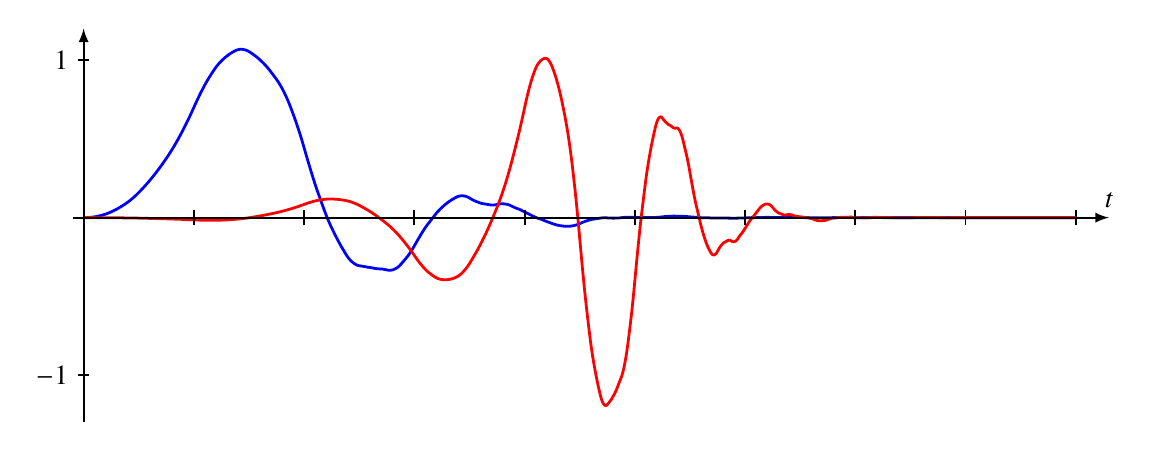
\begin{tikzpicture}[>=latex,yscale=2,xscale=1.4]

\draw[line width=1pt,color=blue] (0.00000, 0.00000)
--(0.00195, 0.00001)
--(0.00391, 0.00001)
--(0.00586, 0.00002)
--(0.00781, 0.00004)
--(0.00977, 0.00005)
--(0.01172, 0.00007)
--(0.01367, 0.00010)
--(0.01562, 0.00013)
--(0.01758, 0.00016)
--(0.01953, 0.00019)
--(0.02148, 0.00023)
--(0.02344, 0.00027)
--(0.02539, 0.00032)
--(0.02734, 0.00037)
--(0.02930, 0.00043)
--(0.03125, 0.00049)
--(0.03320, 0.00055)
--(0.03516, 0.00062)
--(0.03711, 0.00069)
--(0.03906, 0.00076)
--(0.04102, 0.00084)
--(0.04297, 0.00092)
--(0.04492, 0.00100)
--(0.04688, 0.00109)
--(0.04883, 0.00118)
--(0.05078, 0.00128)
--(0.05273, 0.00138)
--(0.05469, 0.00149)
--(0.05664, 0.00161)
--(0.05859, 0.00173)
--(0.06055, 0.00185)
--(0.06250, 0.00199)
--(0.06445, 0.00212)
--(0.06641, 0.00226)
--(0.06836, 0.00240)
--(0.07031, 0.00254)
--(0.07227, 0.00269)
--(0.07422, 0.00284)
--(0.07617, 0.00300)
--(0.07812, 0.00315)
--(0.08008, 0.00332)
--(0.08203, 0.00348)
--(0.08398, 0.00365)
--(0.08594, 0.00383)
--(0.08789, 0.00401)
--(0.08984, 0.00419)
--(0.09180, 0.00437)
--(0.09375, 0.00456)
--(0.09570, 0.00476)
--(0.09766, 0.00496)
--(0.09961, 0.00517)
--(0.10156, 0.00538)
--(0.10352, 0.00560)
--(0.10547, 0.00583)
--(0.10742, 0.00606)
--(0.10938, 0.00630)
--(0.11133, 0.00655)
--(0.11328, 0.00680)
--(0.11523, 0.00705)
--(0.11719, 0.00731)
--(0.11914, 0.00758)
--(0.12109, 0.00785)
--(0.12305, 0.00814)
--(0.12500, 0.00842)
--(0.12695, 0.00871)
--(0.12891, 0.00900)
--(0.13086, 0.00930)
--(0.13281, 0.00960)
--(0.13477, 0.00991)
--(0.13672, 0.01021)
--(0.13867, 0.01052)
--(0.14062, 0.01084)
--(0.14258, 0.01116)
--(0.14453, 0.01148)
--(0.14648, 0.01181)
--(0.14844, 0.01214)
--(0.15039, 0.01248)
--(0.15234, 0.01282)
--(0.15430, 0.01316)
--(0.15625, 0.01351)
--(0.15820, 0.01386)
--(0.16016, 0.01422)
--(0.16211, 0.01458)
--(0.16406, 0.01494)
--(0.16602, 0.01531)
--(0.16797, 0.01569)
--(0.16992, 0.01607)
--(0.17188, 0.01645)
--(0.17383, 0.01684)
--(0.17578, 0.01723)
--(0.17773, 0.01762)
--(0.17969, 0.01802)
--(0.18164, 0.01842)
--(0.18359, 0.01882)
--(0.18555, 0.01923)
--(0.18750, 0.01964)
--(0.18945, 0.02006)
--(0.19141, 0.02049)
--(0.19336, 0.02092)
--(0.19531, 0.02136)
--(0.19727, 0.02181)
--(0.19922, 0.02226)
--(0.20117, 0.02272)
--(0.20312, 0.02319)
--(0.20508, 0.02367)
--(0.20703, 0.02415)
--(0.20898, 0.02463)
--(0.21094, 0.02513)
--(0.21289, 0.02563)
--(0.21484, 0.02614)
--(0.21680, 0.02666)
--(0.21875, 0.02719)
--(0.22070, 0.02772)
--(0.22266, 0.02826)
--(0.22461, 0.02880)
--(0.22656, 0.02935)
--(0.22852, 0.02991)
--(0.23047, 0.03047)
--(0.23242, 0.03103)
--(0.23438, 0.03160)
--(0.23633, 0.03218)
--(0.23828, 0.03277)
--(0.24023, 0.03336)
--(0.24219, 0.03396)
--(0.24414, 0.03457)
--(0.24609, 0.03519)
--(0.24805, 0.03581)
--(0.25000, 0.03644)
--(0.25195, 0.03707)
--(0.25391, 0.03771)
--(0.25586, 0.03835)
--(0.25781, 0.03899)
--(0.25977, 0.03964)
--(0.26172, 0.04029)
--(0.26367, 0.04095)
--(0.26562, 0.04161)
--(0.26758, 0.04228)
--(0.26953, 0.04295)
--(0.27148, 0.04362)
--(0.27344, 0.04430)
--(0.27539, 0.04498)
--(0.27734, 0.04566)
--(0.27930, 0.04635)
--(0.28125, 0.04704)
--(0.28320, 0.04773)
--(0.28516, 0.04844)
--(0.28711, 0.04914)
--(0.28906, 0.04985)
--(0.29102, 0.05057)
--(0.29297, 0.05129)
--(0.29492, 0.05202)
--(0.29688, 0.05275)
--(0.29883, 0.05349)
--(0.30078, 0.05423)
--(0.30273, 0.05497)
--(0.30469, 0.05572)
--(0.30664, 0.05647)
--(0.30859, 0.05722)
--(0.31055, 0.05798)
--(0.31250, 0.05874)
--(0.31445, 0.05951)
--(0.31641, 0.06028)
--(0.31836, 0.06106)
--(0.32031, 0.06184)
--(0.32227, 0.06263)
--(0.32422, 0.06342)
--(0.32617, 0.06422)
--(0.32812, 0.06502)
--(0.33008, 0.06583)
--(0.33203, 0.06665)
--(0.33398, 0.06746)
--(0.33594, 0.06829)
--(0.33789, 0.06912)
--(0.33984, 0.06995)
--(0.34180, 0.07079)
--(0.34375, 0.07163)
--(0.34570, 0.07248)
--(0.34766, 0.07334)
--(0.34961, 0.07419)
--(0.35156, 0.07505)
--(0.35352, 0.07591)
--(0.35547, 0.07678)
--(0.35742, 0.07765)
--(0.35938, 0.07852)
--(0.36133, 0.07940)
--(0.36328, 0.08028)
--(0.36523, 0.08117)
--(0.36719, 0.08206)
--(0.36914, 0.08295)
--(0.37109, 0.08385)
--(0.37305, 0.08475)
--(0.37500, 0.08566)
--(0.37695, 0.08657)
--(0.37891, 0.08749)
--(0.38086, 0.08842)
--(0.38281, 0.08936)
--(0.38477, 0.09030)
--(0.38672, 0.09125)
--(0.38867, 0.09221)
--(0.39062, 0.09318)
--(0.39258, 0.09415)
--(0.39453, 0.09513)
--(0.39648, 0.09612)
--(0.39844, 0.09712)
--(0.40039, 0.09812)
--(0.40234, 0.09913)
--(0.40430, 0.10016)
--(0.40625, 0.10119)
--(0.40820, 0.10222)
--(0.41016, 0.10326)
--(0.41211, 0.10432)
--(0.41406, 0.10537)
--(0.41602, 0.10644)
--(0.41797, 0.10751)
--(0.41992, 0.10859)
--(0.42188, 0.10968)
--(0.42383, 0.11077)
--(0.42578, 0.11188)
--(0.42773, 0.11299)
--(0.42969, 0.11412)
--(0.43164, 0.11525)
--(0.43359, 0.11639)
--(0.43555, 0.11754)
--(0.43750, 0.11870)
--(0.43945, 0.11987)
--(0.44141, 0.12104)
--(0.44336, 0.12221)
--(0.44531, 0.12340)
--(0.44727, 0.12459)
--(0.44922, 0.12578)
--(0.45117, 0.12698)
--(0.45312, 0.12819)
--(0.45508, 0.12940)
--(0.45703, 0.13062)
--(0.45898, 0.13185)
--(0.46094, 0.13308)
--(0.46289, 0.13432)
--(0.46484, 0.13556)
--(0.46680, 0.13681)
--(0.46875, 0.13807)
--(0.47070, 0.13933)
--(0.47266, 0.14060)
--(0.47461, 0.14188)
--(0.47656, 0.14317)
--(0.47852, 0.14447)
--(0.48047, 0.14578)
--(0.48242, 0.14709)
--(0.48438, 0.14842)
--(0.48633, 0.14975)
--(0.48828, 0.15109)
--(0.49023, 0.15243)
--(0.49219, 0.15378)
--(0.49414, 0.15514)
--(0.49609, 0.15651)
--(0.49805, 0.15789)
--(0.50000, 0.15927)
--(0.50195, 0.16066)
--(0.50391, 0.16205)
--(0.50586, 0.16345)
--(0.50781, 0.16485)
--(0.50977, 0.16626)
--(0.51172, 0.16767)
--(0.51367, 0.16908)
--(0.51562, 0.17050)
--(0.51758, 0.17193)
--(0.51953, 0.17336)
--(0.52148, 0.17479)
--(0.52344, 0.17624)
--(0.52539, 0.17768)
--(0.52734, 0.17913)
--(0.52930, 0.18058)
--(0.53125, 0.18204)
--(0.53320, 0.18350)
--(0.53516, 0.18497)
--(0.53711, 0.18644)
--(0.53906, 0.18792)
--(0.54102, 0.18940)
--(0.54297, 0.19088)
--(0.54492, 0.19238)
--(0.54688, 0.19387)
--(0.54883, 0.19537)
--(0.55078, 0.19687)
--(0.55273, 0.19837)
--(0.55469, 0.19988)
--(0.55664, 0.20139)
--(0.55859, 0.20290)
--(0.56055, 0.20441)
--(0.56250, 0.20593)
--(0.56445, 0.20746)
--(0.56641, 0.20899)
--(0.56836, 0.21053)
--(0.57031, 0.21207)
--(0.57227, 0.21362)
--(0.57422, 0.21518)
--(0.57617, 0.21674)
--(0.57812, 0.21831)
--(0.58008, 0.21988)
--(0.58203, 0.22146)
--(0.58398, 0.22304)
--(0.58594, 0.22463)
--(0.58789, 0.22623)
--(0.58984, 0.22783)
--(0.59180, 0.22944)
--(0.59375, 0.23106)
--(0.59570, 0.23268)
--(0.59766, 0.23430)
--(0.59961, 0.23593)
--(0.60156, 0.23756)
--(0.60352, 0.23919)
--(0.60547, 0.24083)
--(0.60742, 0.24247)
--(0.60938, 0.24411)
--(0.61133, 0.24576)
--(0.61328, 0.24741)
--(0.61523, 0.24907)
--(0.61719, 0.25073)
--(0.61914, 0.25240)
--(0.62109, 0.25407)
--(0.62305, 0.25575)
--(0.62500, 0.25743)
--(0.62695, 0.25911)
--(0.62891, 0.26081)
--(0.63086, 0.26250)
--(0.63281, 0.26420)
--(0.63477, 0.26591)
--(0.63672, 0.26763)
--(0.63867, 0.26935)
--(0.64062, 0.27107)
--(0.64258, 0.27281)
--(0.64453, 0.27454)
--(0.64648, 0.27628)
--(0.64844, 0.27803)
--(0.65039, 0.27978)
--(0.65234, 0.28154)
--(0.65430, 0.28330)
--(0.65625, 0.28507)
--(0.65820, 0.28684)
--(0.66016, 0.28862)
--(0.66211, 0.29041)
--(0.66406, 0.29220)
--(0.66602, 0.29400)
--(0.66797, 0.29580)
--(0.66992, 0.29761)
--(0.67188, 0.29942)
--(0.67383, 0.30124)
--(0.67578, 0.30307)
--(0.67773, 0.30490)
--(0.67969, 0.30674)
--(0.68164, 0.30858)
--(0.68359, 0.31043)
--(0.68555, 0.31229)
--(0.68750, 0.31415)
--(0.68945, 0.31602)
--(0.69141, 0.31789)
--(0.69336, 0.31977)
--(0.69531, 0.32164)
--(0.69727, 0.32353)
--(0.69922, 0.32541)
--(0.70117, 0.32730)
--(0.70312, 0.32920)
--(0.70508, 0.33109)
--(0.70703, 0.33300)
--(0.70898, 0.33490)
--(0.71094, 0.33681)
--(0.71289, 0.33873)
--(0.71484, 0.34064)
--(0.71680, 0.34256)
--(0.71875, 0.34449)
--(0.72070, 0.34642)
--(0.72266, 0.34835)
--(0.72461, 0.35029)
--(0.72656, 0.35223)
--(0.72852, 0.35418)
--(0.73047, 0.35614)
--(0.73242, 0.35810)
--(0.73438, 0.36006)
--(0.73633, 0.36203)
--(0.73828, 0.36400)
--(0.74023, 0.36598)
--(0.74219, 0.36796)
--(0.74414, 0.36994)
--(0.74609, 0.37193)
--(0.74805, 0.37392)
--(0.75000, 0.37592)
--(0.75195, 0.37792)
--(0.75391, 0.37993)
--(0.75586, 0.38195)
--(0.75781, 0.38398)
--(0.75977, 0.38602)
--(0.76172, 0.38806)
--(0.76367, 0.39012)
--(0.76562, 0.39218)
--(0.76758, 0.39425)
--(0.76953, 0.39632)
--(0.77148, 0.39841)
--(0.77344, 0.40050)
--(0.77539, 0.40261)
--(0.77734, 0.40472)
--(0.77930, 0.40684)
--(0.78125, 0.40898)
--(0.78320, 0.41111)
--(0.78516, 0.41326)
--(0.78711, 0.41541)
--(0.78906, 0.41758)
--(0.79102, 0.41974)
--(0.79297, 0.42192)
--(0.79492, 0.42410)
--(0.79688, 0.42629)
--(0.79883, 0.42849)
--(0.80078, 0.43071)
--(0.80273, 0.43293)
--(0.80469, 0.43516)
--(0.80664, 0.43740)
--(0.80859, 0.43965)
--(0.81055, 0.44191)
--(0.81250, 0.44417)
--(0.81445, 0.44645)
--(0.81641, 0.44873)
--(0.81836, 0.45102)
--(0.82031, 0.45332)
--(0.82227, 0.45563)
--(0.82422, 0.45794)
--(0.82617, 0.46027)
--(0.82812, 0.46260)
--(0.83008, 0.46493)
--(0.83203, 0.46728)
--(0.83398, 0.46964)
--(0.83594, 0.47200)
--(0.83789, 0.47437)
--(0.83984, 0.47674)
--(0.84180, 0.47913)
--(0.84375, 0.48152)
--(0.84570, 0.48392)
--(0.84766, 0.48634)
--(0.84961, 0.48876)
--(0.85156, 0.49119)
--(0.85352, 0.49364)
--(0.85547, 0.49609)
--(0.85742, 0.49856)
--(0.85938, 0.50104)
--(0.86133, 0.50352)
--(0.86328, 0.50602)
--(0.86523, 0.50852)
--(0.86719, 0.51104)
--(0.86914, 0.51356)
--(0.87109, 0.51610)
--(0.87305, 0.51864)
--(0.87500, 0.52120)
--(0.87695, 0.52376)
--(0.87891, 0.52633)
--(0.88086, 0.52890)
--(0.88281, 0.53148)
--(0.88477, 0.53407)
--(0.88672, 0.53666)
--(0.88867, 0.53926)
--(0.89062, 0.54187)
--(0.89258, 0.54448)
--(0.89453, 0.54710)
--(0.89648, 0.54973)
--(0.89844, 0.55237)
--(0.90039, 0.55501)
--(0.90234, 0.55766)
--(0.90430, 0.56031)
--(0.90625, 0.56297)
--(0.90820, 0.56564)
--(0.91016, 0.56831)
--(0.91211, 0.57099)
--(0.91406, 0.57368)
--(0.91602, 0.57638)
--(0.91797, 0.57908)
--(0.91992, 0.58180)
--(0.92188, 0.58452)
--(0.92383, 0.58724)
--(0.92578, 0.58997)
--(0.92773, 0.59270)
--(0.92969, 0.59544)
--(0.93164, 0.59819)
--(0.93359, 0.60094)
--(0.93555, 0.60370)
--(0.93750, 0.60646)
--(0.93945, 0.60924)
--(0.94141, 0.61202)
--(0.94336, 0.61482)
--(0.94531, 0.61762)
--(0.94727, 0.62043)
--(0.94922, 0.62325)
--(0.95117, 0.62608)
--(0.95312, 0.62893)
--(0.95508, 0.63178)
--(0.95703, 0.63464)
--(0.95898, 0.63750)
--(0.96094, 0.64038)
--(0.96289, 0.64327)
--(0.96484, 0.64617)
--(0.96680, 0.64908)
--(0.96875, 0.65200)
--(0.97070, 0.65493)
--(0.97266, 0.65787)
--(0.97461, 0.66081)
--(0.97656, 0.66376)
--(0.97852, 0.66671)
--(0.98047, 0.66967)
--(0.98242, 0.67264)
--(0.98438, 0.67562)
--(0.98633, 0.67861)
--(0.98828, 0.68161)
--(0.99023, 0.68461)
--(0.99219, 0.68763)
--(0.99414, 0.69065)
--(0.99609, 0.69369)
--(0.99805, 0.69673)
--(1.00000, 0.69977)
--(1.00195, 0.70281)
--(1.00391, 0.70584)
--(1.00586, 0.70886)
--(1.00781, 0.71188)
--(1.00977, 0.71490)
--(1.01172, 0.71791)
--(1.01367, 0.72090)
--(1.01562, 0.72389)
--(1.01758, 0.72687)
--(1.01953, 0.72984)
--(1.02148, 0.73281)
--(1.02344, 0.73577)
--(1.02539, 0.73871)
--(1.02734, 0.74164)
--(1.02930, 0.74455)
--(1.03125, 0.74745)
--(1.03320, 0.75035)
--(1.03516, 0.75324)
--(1.03711, 0.75613)
--(1.03906, 0.75901)
--(1.04102, 0.76188)
--(1.04297, 0.76475)
--(1.04492, 0.76761)
--(1.04688, 0.77046)
--(1.04883, 0.77330)
--(1.05078, 0.77611)
--(1.05273, 0.77891)
--(1.05469, 0.78169)
--(1.05664, 0.78445)
--(1.05859, 0.78721)
--(1.06055, 0.78994)
--(1.06250, 0.79266)
--(1.06445, 0.79538)
--(1.06641, 0.79809)
--(1.06836, 0.80079)
--(1.07031, 0.80348)
--(1.07227, 0.80617)
--(1.07422, 0.80884)
--(1.07617, 0.81151)
--(1.07812, 0.81417)
--(1.08008, 0.81682)
--(1.08203, 0.81945)
--(1.08398, 0.82208)
--(1.08594, 0.82470)
--(1.08789, 0.82731)
--(1.08984, 0.82992)
--(1.09180, 0.83252)
--(1.09375, 0.83510)
--(1.09570, 0.83767)
--(1.09766, 0.84021)
--(1.09961, 0.84273)
--(1.10156, 0.84524)
--(1.10352, 0.84772)
--(1.10547, 0.85018)
--(1.10742, 0.85262)
--(1.10938, 0.85504)
--(1.11133, 0.85744)
--(1.11328, 0.85983)
--(1.11523, 0.86220)
--(1.11719, 0.86455)
--(1.11914, 0.86688)
--(1.12109, 0.86919)
--(1.12305, 0.87147)
--(1.12500, 0.87375)
--(1.12695, 0.87601)
--(1.12891, 0.87827)
--(1.13086, 0.88052)
--(1.13281, 0.88276)
--(1.13477, 0.88500)
--(1.13672, 0.88723)
--(1.13867, 0.88946)
--(1.14062, 0.89168)
--(1.14258, 0.89388)
--(1.14453, 0.89608)
--(1.14648, 0.89826)
--(1.14844, 0.90044)
--(1.15039, 0.90261)
--(1.15234, 0.90478)
--(1.15430, 0.90694)
--(1.15625, 0.90909)
--(1.15820, 0.91123)
--(1.16016, 0.91335)
--(1.16211, 0.91547)
--(1.16406, 0.91758)
--(1.16602, 0.91967)
--(1.16797, 0.92175)
--(1.16992, 0.92382)
--(1.17188, 0.92588)
--(1.17383, 0.92793)
--(1.17578, 0.92998)
--(1.17773, 0.93203)
--(1.17969, 0.93407)
--(1.18164, 0.93610)
--(1.18359, 0.93813)
--(1.18555, 0.94015)
--(1.18750, 0.94216)
--(1.18945, 0.94415)
--(1.19141, 0.94611)
--(1.19336, 0.94805)
--(1.19531, 0.94997)
--(1.19727, 0.95188)
--(1.19922, 0.95375)
--(1.20117, 0.95560)
--(1.20312, 0.95743)
--(1.20508, 0.95924)
--(1.20703, 0.96103)
--(1.20898, 0.96280)
--(1.21094, 0.96455)
--(1.21289, 0.96626)
--(1.21484, 0.96795)
--(1.21680, 0.96961)
--(1.21875, 0.97124)
--(1.22070, 0.97287)
--(1.22266, 0.97447)
--(1.22461, 0.97607)
--(1.22656, 0.97765)
--(1.22852, 0.97921)
--(1.23047, 0.98076)
--(1.23242, 0.98229)
--(1.23438, 0.98381)
--(1.23633, 0.98530)
--(1.23828, 0.98677)
--(1.24023, 0.98821)
--(1.24219, 0.98963)
--(1.24414, 0.99103)
--(1.24609, 0.99241)
--(1.24805, 0.99376)
--(1.25000, 0.99510)
--(1.25195, 0.99643)
--(1.25391, 0.99775)
--(1.25586, 0.99906)
--(1.25781, 1.00036)
--(1.25977, 1.00164)
--(1.26172, 1.00292)
--(1.26367, 1.00419)
--(1.26562, 1.00545)
--(1.26758, 1.00670)
--(1.26953, 1.00794)
--(1.27148, 1.00917)
--(1.27344, 1.01040)
--(1.27539, 1.01162)
--(1.27734, 1.01284)
--(1.27930, 1.01405)
--(1.28125, 1.01526)
--(1.28320, 1.01645)
--(1.28516, 1.01763)
--(1.28711, 1.01879)
--(1.28906, 1.01993)
--(1.29102, 1.02106)
--(1.29297, 1.02218)
--(1.29492, 1.02328)
--(1.29688, 1.02436)
--(1.29883, 1.02545)
--(1.30078, 1.02652)
--(1.30273, 1.02760)
--(1.30469, 1.02866)
--(1.30664, 1.02971)
--(1.30859, 1.03076)
--(1.31055, 1.03179)
--(1.31250, 1.03282)
--(1.31445, 1.03383)
--(1.31641, 1.03483)
--(1.31836, 1.03581)
--(1.32031, 1.03678)
--(1.32227, 1.03775)
--(1.32422, 1.03870)
--(1.32617, 1.03963)
--(1.32812, 1.04056)
--(1.33008, 1.04147)
--(1.33203, 1.04237)
--(1.33398, 1.04325)
--(1.33594, 1.04412)
--(1.33789, 1.04498)
--(1.33984, 1.04582)
--(1.34180, 1.04664)
--(1.34375, 1.04746)
--(1.34570, 1.04826)
--(1.34766, 1.04906)
--(1.34961, 1.04986)
--(1.35156, 1.05065)
--(1.35352, 1.05143)
--(1.35547, 1.05220)
--(1.35742, 1.05298)
--(1.35938, 1.05374)
--(1.36133, 1.05449)
--(1.36328, 1.05523)
--(1.36523, 1.05597)
--(1.36719, 1.05669)
--(1.36914, 1.05741)
--(1.37109, 1.05812)
--(1.37305, 1.05883)
--(1.37500, 1.05952)
--(1.37695, 1.06018)
--(1.37891, 1.06083)
--(1.38086, 1.06145)
--(1.38281, 1.06205)
--(1.38477, 1.06263)
--(1.38672, 1.06318)
--(1.38867, 1.06369)
--(1.39062, 1.06419)
--(1.39258, 1.06466)
--(1.39453, 1.06512)
--(1.39648, 1.06556)
--(1.39844, 1.06596)
--(1.40039, 1.06634)
--(1.40234, 1.06669)
--(1.40430, 1.06701)
--(1.40625, 1.06731)
--(1.40820, 1.06758)
--(1.41016, 1.06783)
--(1.41211, 1.06806)
--(1.41406, 1.06827)
--(1.41602, 1.06846)
--(1.41797, 1.06862)
--(1.41992, 1.06877)
--(1.42188, 1.06889)
--(1.42383, 1.06897)
--(1.42578, 1.06903)
--(1.42773, 1.06905)
--(1.42969, 1.06903)
--(1.43164, 1.06900)
--(1.43359, 1.06893)
--(1.43555, 1.06883)
--(1.43750, 1.06870)
--(1.43945, 1.06856)
--(1.44141, 1.06840)
--(1.44336, 1.06822)
--(1.44531, 1.06803)
--(1.44727, 1.06782)
--(1.44922, 1.06759)
--(1.45117, 1.06735)
--(1.45312, 1.06708)
--(1.45508, 1.06680)
--(1.45703, 1.06650)
--(1.45898, 1.06618)
--(1.46094, 1.06584)
--(1.46289, 1.06549)
--(1.46484, 1.06513)
--(1.46680, 1.06475)
--(1.46875, 1.06435)
--(1.47070, 1.06393)
--(1.47266, 1.06347)
--(1.47461, 1.06299)
--(1.47656, 1.06247)
--(1.47852, 1.06193)
--(1.48047, 1.06136)
--(1.48242, 1.06076)
--(1.48438, 1.06013)
--(1.48633, 1.05948)
--(1.48828, 1.05881)
--(1.49023, 1.05813)
--(1.49219, 1.05742)
--(1.49414, 1.05667)
--(1.49609, 1.05591)
--(1.49805, 1.05512)
--(1.50000, 1.05431)
--(1.50195, 1.05349)
--(1.50391, 1.05266)
--(1.50586, 1.05182)
--(1.50781, 1.05097)
--(1.50977, 1.05011)
--(1.51172, 1.04924)
--(1.51367, 1.04837)
--(1.51562, 1.04750)
--(1.51758, 1.04660)
--(1.51953, 1.04569)
--(1.52148, 1.04477)
--(1.52344, 1.04384)
--(1.52539, 1.04291)
--(1.52734, 1.04197)
--(1.52930, 1.04103)
--(1.53125, 1.04008)
--(1.53320, 1.03912)
--(1.53516, 1.03815)
--(1.53711, 1.03717)
--(1.53906, 1.03618)
--(1.54102, 1.03518)
--(1.54297, 1.03418)
--(1.54492, 1.03316)
--(1.54688, 1.03214)
--(1.54883, 1.03112)
--(1.55078, 1.03010)
--(1.55273, 1.02908)
--(1.55469, 1.02806)
--(1.55664, 1.02704)
--(1.55859, 1.02602)
--(1.56055, 1.02500)
--(1.56250, 1.02398)
--(1.56445, 1.02293)
--(1.56641, 1.02188)
--(1.56836, 1.02080)
--(1.57031, 1.01971)
--(1.57227, 1.01861)
--(1.57422, 1.01750)
--(1.57617, 1.01636)
--(1.57812, 1.01521)
--(1.58008, 1.01405)
--(1.58203, 1.01288)
--(1.58398, 1.01170)
--(1.58594, 1.01050)
--(1.58789, 1.00928)
--(1.58984, 1.00805)
--(1.59180, 1.00679)
--(1.59375, 1.00553)
--(1.59570, 1.00427)
--(1.59766, 1.00300)
--(1.59961, 1.00173)
--(1.60156, 1.00046)
--(1.60352, 0.99918)
--(1.60547, 0.99791)
--(1.60742, 0.99664)
--(1.60938, 0.99537)
--(1.61133, 0.99408)
--(1.61328, 0.99279)
--(1.61523, 0.99148)
--(1.61719, 0.99016)
--(1.61914, 0.98884)
--(1.62109, 0.98752)
--(1.62305, 0.98619)
--(1.62500, 0.98486)
--(1.62695, 0.98351)
--(1.62891, 0.98215)
--(1.63086, 0.98078)
--(1.63281, 0.97940)
--(1.63477, 0.97800)
--(1.63672, 0.97659)
--(1.63867, 0.97515)
--(1.64062, 0.97371)
--(1.64258, 0.97226)
--(1.64453, 0.97080)
--(1.64648, 0.96933)
--(1.64844, 0.96786)
--(1.65039, 0.96636)
--(1.65234, 0.96486)
--(1.65430, 0.96334)
--(1.65625, 0.96181)
--(1.65820, 0.96027)
--(1.66016, 0.95871)
--(1.66211, 0.95714)
--(1.66406, 0.95556)
--(1.66602, 0.95397)
--(1.66797, 0.95237)
--(1.66992, 0.95075)
--(1.67188, 0.94912)
--(1.67383, 0.94748)
--(1.67578, 0.94582)
--(1.67773, 0.94414)
--(1.67969, 0.94245)
--(1.68164, 0.94074)
--(1.68359, 0.93902)
--(1.68555, 0.93728)
--(1.68750, 0.93553)
--(1.68945, 0.93377)
--(1.69141, 0.93202)
--(1.69336, 0.93026)
--(1.69531, 0.92849)
--(1.69727, 0.92673)
--(1.69922, 0.92496)
--(1.70117, 0.92319)
--(1.70312, 0.92141)
--(1.70508, 0.91963)
--(1.70703, 0.91785)
--(1.70898, 0.91606)
--(1.71094, 0.91427)
--(1.71289, 0.91248)
--(1.71484, 0.91069)
--(1.71680, 0.90890)
--(1.71875, 0.90710)
--(1.72070, 0.90530)
--(1.72266, 0.90349)
--(1.72461, 0.90166)
--(1.72656, 0.89983)
--(1.72852, 0.89800)
--(1.73047, 0.89615)
--(1.73242, 0.89429)
--(1.73438, 0.89242)
--(1.73633, 0.89055)
--(1.73828, 0.88869)
--(1.74023, 0.88682)
--(1.74219, 0.88495)
--(1.74414, 0.88307)
--(1.74609, 0.88119)
--(1.74805, 0.87930)
--(1.75000, 0.87740)
--(1.75195, 0.87548)
--(1.75391, 0.87354)
--(1.75586, 0.87158)
--(1.75781, 0.86959)
--(1.75977, 0.86759)
--(1.76172, 0.86556)
--(1.76367, 0.86351)
--(1.76562, 0.86143)
--(1.76758, 0.85933)
--(1.76953, 0.85720)
--(1.77148, 0.85506)
--(1.77344, 0.85289)
--(1.77539, 0.85068)
--(1.77734, 0.84844)
--(1.77930, 0.84617)
--(1.78125, 0.84388)
--(1.78320, 0.84157)
--(1.78516, 0.83924)
--(1.78711, 0.83689)
--(1.78906, 0.83453)
--(1.79102, 0.83214)
--(1.79297, 0.82973)
--(1.79492, 0.82731)
--(1.79688, 0.82487)
--(1.79883, 0.82239)
--(1.80078, 0.81988)
--(1.80273, 0.81733)
--(1.80469, 0.81475)
--(1.80664, 0.81215)
--(1.80859, 0.80952)
--(1.81055, 0.80686)
--(1.81250, 0.80418)
--(1.81445, 0.80147)
--(1.81641, 0.79874)
--(1.81836, 0.79600)
--(1.82031, 0.79323)
--(1.82227, 0.79044)
--(1.82422, 0.78763)
--(1.82617, 0.78479)
--(1.82812, 0.78194)
--(1.83008, 0.77906)
--(1.83203, 0.77616)
--(1.83398, 0.77324)
--(1.83594, 0.77030)
--(1.83789, 0.76733)
--(1.83984, 0.76436)
--(1.84180, 0.76136)
--(1.84375, 0.75833)
--(1.84570, 0.75528)
--(1.84766, 0.75219)
--(1.84961, 0.74906)
--(1.85156, 0.74590)
--(1.85352, 0.74271)
--(1.85547, 0.73949)
--(1.85742, 0.73622)
--(1.85938, 0.73293)
--(1.86133, 0.72961)
--(1.86328, 0.72626)
--(1.86523, 0.72288)
--(1.86719, 0.71947)
--(1.86914, 0.71603)
--(1.87109, 0.71255)
--(1.87305, 0.70904)
--(1.87500, 0.70551)
--(1.87695, 0.70196)
--(1.87891, 0.69839)
--(1.88086, 0.69481)
--(1.88281, 0.69121)
--(1.88477, 0.68760)
--(1.88672, 0.68398)
--(1.88867, 0.68035)
--(1.89062, 0.67671)
--(1.89258, 0.67304)
--(1.89453, 0.66936)
--(1.89648, 0.66565)
--(1.89844, 0.66193)
--(1.90039, 0.65821)
--(1.90234, 0.65447)
--(1.90430, 0.65073)
--(1.90625, 0.64696)
--(1.90820, 0.64318)
--(1.91016, 0.63938)
--(1.91211, 0.63556)
--(1.91406, 0.63173)
--(1.91602, 0.62788)
--(1.91797, 0.62400)
--(1.91992, 0.62011)
--(1.92188, 0.61620)
--(1.92383, 0.61229)
--(1.92578, 0.60837)
--(1.92773, 0.60444)
--(1.92969, 0.60050)
--(1.93164, 0.59655)
--(1.93359, 0.59259)
--(1.93555, 0.58863)
--(1.93750, 0.58464)
--(1.93945, 0.58063)
--(1.94141, 0.57659)
--(1.94336, 0.57252)
--(1.94531, 0.56842)
--(1.94727, 0.56430)
--(1.94922, 0.56014)
--(1.95117, 0.55596)
--(1.95312, 0.55175)
--(1.95508, 0.54751)
--(1.95703, 0.54325)
--(1.95898, 0.53897)
--(1.96094, 0.53465)
--(1.96289, 0.53030)
--(1.96484, 0.52591)
--(1.96680, 0.52149)
--(1.96875, 0.51704)
--(1.97070, 0.51258)
--(1.97266, 0.50811)
--(1.97461, 0.50361)
--(1.97656, 0.49910)
--(1.97852, 0.49457)
--(1.98047, 0.49003)
--(1.98242, 0.48548)
--(1.98438, 0.48090)
--(1.98633, 0.47630)
--(1.98828, 0.47167)
--(1.99023, 0.46700)
--(1.99219, 0.46232)
--(1.99414, 0.45761)
--(1.99609, 0.45289)
--(1.99805, 0.44813)
--(2.00000, 0.44337)
--(2.00195, 0.43861)
--(2.00391, 0.43385)
--(2.00586, 0.42911)
--(2.00781, 0.42436)
--(2.00977, 0.41961)
--(2.01172, 0.41487)
--(2.01367, 0.41013)
--(2.01562, 0.40541)
--(2.01758, 0.40069)
--(2.01953, 0.39598)
--(2.02148, 0.39127)
--(2.02344, 0.38658)
--(2.02539, 0.38191)
--(2.02734, 0.37726)
--(2.02930, 0.37263)
--(2.03125, 0.36801)
--(2.03320, 0.36339)
--(2.03516, 0.35877)
--(2.03711, 0.35414)
--(2.03906, 0.34952)
--(2.04102, 0.34491)
--(2.04297, 0.34030)
--(2.04492, 0.33568)
--(2.04688, 0.33108)
--(2.04883, 0.32650)
--(2.05078, 0.32195)
--(2.05273, 0.31742)
--(2.05469, 0.31291)
--(2.05664, 0.30841)
--(2.05859, 0.30392)
--(2.06055, 0.29947)
--(2.06250, 0.29502)
--(2.06445, 0.29058)
--(2.06641, 0.28615)
--(2.06836, 0.28172)
--(2.07031, 0.27730)
--(2.07227, 0.27290)
--(2.07422, 0.26850)
--(2.07617, 0.26412)
--(2.07812, 0.25974)
--(2.08008, 0.25537)
--(2.08203, 0.25102)
--(2.08398, 0.24668)
--(2.08594, 0.24234)
--(2.08789, 0.23801)
--(2.08984, 0.23369)
--(2.09180, 0.22938)
--(2.09375, 0.22508)
--(2.09570, 0.22081)
--(2.09766, 0.21657)
--(2.09961, 0.21236)
--(2.10156, 0.20818)
--(2.10352, 0.20403)
--(2.10547, 0.19991)
--(2.10742, 0.19583)
--(2.10938, 0.19177)
--(2.11133, 0.18774)
--(2.11328, 0.18373)
--(2.11523, 0.17974)
--(2.11719, 0.17577)
--(2.11914, 0.17185)
--(2.12109, 0.16795)
--(2.12305, 0.16409)
--(2.12500, 0.16024)
--(2.12695, 0.15640)
--(2.12891, 0.15256)
--(2.13086, 0.14873)
--(2.13281, 0.14490)
--(2.13477, 0.14107)
--(2.13672, 0.13724)
--(2.13867, 0.13339)
--(2.14062, 0.12955)
--(2.14258, 0.12573)
--(2.14453, 0.12192)
--(2.14648, 0.11812)
--(2.14844, 0.11432)
--(2.15039, 0.11051)
--(2.15234, 0.10671)
--(2.15430, 0.10290)
--(2.15625, 0.09909)
--(2.15820, 0.09530)
--(2.16016, 0.09152)
--(2.16211, 0.08775)
--(2.16406, 0.08399)
--(2.16602, 0.08024)
--(2.16797, 0.07650)
--(2.16992, 0.07279)
--(2.17188, 0.06907)
--(2.17383, 0.06535)
--(2.17578, 0.06163)
--(2.17773, 0.05790)
--(2.17969, 0.05417)
--(2.18164, 0.05044)
--(2.18359, 0.04671)
--(2.18555, 0.04298)
--(2.18750, 0.03926)
--(2.18945, 0.03557)
--(2.19141, 0.03191)
--(2.19336, 0.02829)
--(2.19531, 0.02469)
--(2.19727, 0.02111)
--(2.19922, 0.01757)
--(2.20117, 0.01406)
--(2.20312, 0.01058)
--(2.20508, 0.00713)
--(2.20703, 0.00371)
--(2.20898, 0.00031)
--(2.21094, -0.00305)
--(2.21289, -0.00637)
--(2.21484, -0.00965)
--(2.21680, -0.01288)
--(2.21875, -0.01609)
--(2.22070, -0.01929)
--(2.22266, -0.02247)
--(2.22461, -0.02564)
--(2.22656, -0.02879)
--(2.22852, -0.03193)
--(2.23047, -0.03505)
--(2.23242, -0.03817)
--(2.23438, -0.04126)
--(2.23633, -0.04432)
--(2.23828, -0.04734)
--(2.24023, -0.05033)
--(2.24219, -0.05328)
--(2.24414, -0.05622)
--(2.24609, -0.05914)
--(2.24805, -0.06202)
--(2.25000, -0.06489)
--(2.25195, -0.06774)
--(2.25391, -0.07058)
--(2.25586, -0.07342)
--(2.25781, -0.07625)
--(2.25977, -0.07906)
--(2.26172, -0.08186)
--(2.26367, -0.08465)
--(2.26562, -0.08744)
--(2.26758, -0.09022)
--(2.26953, -0.09299)
--(2.27148, -0.09575)
--(2.27344, -0.09851)
--(2.27539, -0.10127)
--(2.27734, -0.10404)
--(2.27930, -0.10680)
--(2.28125, -0.10956)
--(2.28320, -0.11230)
--(2.28516, -0.11502)
--(2.28711, -0.11771)
--(2.28906, -0.12039)
--(2.29102, -0.12306)
--(2.29297, -0.12571)
--(2.29492, -0.12833)
--(2.29688, -0.13094)
--(2.29883, -0.13355)
--(2.30078, -0.13616)
--(2.30273, -0.13877)
--(2.30469, -0.14136)
--(2.30664, -0.14395)
--(2.30859, -0.14652)
--(2.31055, -0.14909)
--(2.31250, -0.15164)
--(2.31445, -0.15418)
--(2.31641, -0.15671)
--(2.31836, -0.15923)
--(2.32031, -0.16173)
--(2.32227, -0.16422)
--(2.32422, -0.16670)
--(2.32617, -0.16918)
--(2.32812, -0.17163)
--(2.33008, -0.17408)
--(2.33203, -0.17651)
--(2.33398, -0.17892)
--(2.33594, -0.18132)
--(2.33789, -0.18371)
--(2.33984, -0.18608)
--(2.34180, -0.18843)
--(2.34375, -0.19078)
--(2.34570, -0.19312)
--(2.34766, -0.19545)
--(2.34961, -0.19779)
--(2.35156, -0.20011)
--(2.35352, -0.20244)
--(2.35547, -0.20476)
--(2.35742, -0.20708)
--(2.35938, -0.20939)
--(2.36133, -0.21169)
--(2.36328, -0.21399)
--(2.36523, -0.21628)
--(2.36719, -0.21856)
--(2.36914, -0.22084)
--(2.37109, -0.22312)
--(2.37305, -0.22539)
--(2.37500, -0.22765)
--(2.37695, -0.22988)
--(2.37891, -0.23208)
--(2.38086, -0.23424)
--(2.38281, -0.23637)
--(2.38477, -0.23848)
--(2.38672, -0.24055)
--(2.38867, -0.24257)
--(2.39062, -0.24456)
--(2.39258, -0.24653)
--(2.39453, -0.24847)
--(2.39648, -0.25038)
--(2.39844, -0.25226)
--(2.40039, -0.25409)
--(2.40234, -0.25588)
--(2.40430, -0.25763)
--(2.40625, -0.25935)
--(2.40820, -0.26104)
--(2.41016, -0.26270)
--(2.41211, -0.26434)
--(2.41406, -0.26594)
--(2.41602, -0.26752)
--(2.41797, -0.26906)
--(2.41992, -0.27059)
--(2.42188, -0.27208)
--(2.42383, -0.27352)
--(2.42578, -0.27491)
--(2.42773, -0.27625)
--(2.42969, -0.27756)
--(2.43164, -0.27882)
--(2.43359, -0.28004)
--(2.43555, -0.28122)
--(2.43750, -0.28236)
--(2.43945, -0.28348)
--(2.44141, -0.28458)
--(2.44336, -0.28567)
--(2.44531, -0.28673)
--(2.44727, -0.28776)
--(2.44922, -0.28877)
--(2.45117, -0.28977)
--(2.45312, -0.29074)
--(2.45508, -0.29169)
--(2.45703, -0.29261)
--(2.45898, -0.29350)
--(2.46094, -0.29438)
--(2.46289, -0.29524)
--(2.46484, -0.29609)
--(2.46680, -0.29692)
--(2.46875, -0.29773)
--(2.47070, -0.29849)
--(2.47266, -0.29921)
--(2.47461, -0.29990)
--(2.47656, -0.30054)
--(2.47852, -0.30114)
--(2.48047, -0.30170)
--(2.48242, -0.30221)
--(2.48438, -0.30269)
--(2.48633, -0.30314)
--(2.48828, -0.30357)
--(2.49023, -0.30397)
--(2.49219, -0.30434)
--(2.49414, -0.30467)
--(2.49609, -0.30496)
--(2.49805, -0.30522)
--(2.50000, -0.30546)
--(2.50195, -0.30570)
--(2.50391, -0.30592)
--(2.50586, -0.30614)
--(2.50781, -0.30636)
--(2.50977, -0.30657)
--(2.51172, -0.30679)
--(2.51367, -0.30702)
--(2.51562, -0.30724)
--(2.51758, -0.30745)
--(2.51953, -0.30766)
--(2.52148, -0.30785)
--(2.52344, -0.30804)
--(2.52539, -0.30824)
--(2.52734, -0.30845)
--(2.52930, -0.30867)
--(2.53125, -0.30889)
--(2.53320, -0.30910)
--(2.53516, -0.30931)
--(2.53711, -0.30952)
--(2.53906, -0.30972)
--(2.54102, -0.30993)
--(2.54297, -0.31013)
--(2.54492, -0.31033)
--(2.54688, -0.31053)
--(2.54883, -0.31076)
--(2.55078, -0.31100)
--(2.55273, -0.31126)
--(2.55469, -0.31153)
--(2.55664, -0.31182)
--(2.55859, -0.31212)
--(2.56055, -0.31244)
--(2.56250, -0.31277)
--(2.56445, -0.31308)
--(2.56641, -0.31338)
--(2.56836, -0.31366)
--(2.57031, -0.31393)
--(2.57227, -0.31420)
--(2.57422, -0.31445)
--(2.57617, -0.31468)
--(2.57812, -0.31490)
--(2.58008, -0.31512)
--(2.58203, -0.31533)
--(2.58398, -0.31555)
--(2.58594, -0.31575)
--(2.58789, -0.31592)
--(2.58984, -0.31608)
--(2.59180, -0.31622)
--(2.59375, -0.31636)
--(2.59570, -0.31652)
--(2.59766, -0.31669)
--(2.59961, -0.31687)
--(2.60156, -0.31707)
--(2.60352, -0.31728)
--(2.60547, -0.31751)
--(2.60742, -0.31777)
--(2.60938, -0.31803)
--(2.61133, -0.31829)
--(2.61328, -0.31854)
--(2.61523, -0.31879)
--(2.61719, -0.31905)
--(2.61914, -0.31933)
--(2.62109, -0.31961)
--(2.62305, -0.31990)
--(2.62500, -0.32019)
--(2.62695, -0.32048)
--(2.62891, -0.32076)
--(2.63086, -0.32103)
--(2.63281, -0.32130)
--(2.63477, -0.32155)
--(2.63672, -0.32179)
--(2.63867, -0.32201)
--(2.64062, -0.32223)
--(2.64258, -0.32245)
--(2.64453, -0.32267)
--(2.64648, -0.32289)
--(2.64844, -0.32310)
--(2.65039, -0.32330)
--(2.65234, -0.32349)
--(2.65430, -0.32367)
--(2.65625, -0.32385)
--(2.65820, -0.32402)
--(2.66016, -0.32419)
--(2.66211, -0.32434)
--(2.66406, -0.32449)
--(2.66602, -0.32464)
--(2.66797, -0.32478)
--(2.66992, -0.32492)
--(2.67188, -0.32504)
--(2.67383, -0.32515)
--(2.67578, -0.32525)
--(2.67773, -0.32533)
--(2.67969, -0.32540)
--(2.68164, -0.32546)
--(2.68359, -0.32550)
--(2.68555, -0.32553)
--(2.68750, -0.32556)
--(2.68945, -0.32559)
--(2.69141, -0.32564)
--(2.69336, -0.32570)
--(2.69531, -0.32578)
--(2.69727, -0.32586)
--(2.69922, -0.32596)
--(2.70117, -0.32608)
--(2.70312, -0.32621)
--(2.70508, -0.32635)
--(2.70703, -0.32650)
--(2.70898, -0.32665)
--(2.71094, -0.32681)
--(2.71289, -0.32701)
--(2.71484, -0.32722)
--(2.71680, -0.32745)
--(2.71875, -0.32770)
--(2.72070, -0.32794)
--(2.72266, -0.32819)
--(2.72461, -0.32843)
--(2.72656, -0.32867)
--(2.72852, -0.32892)
--(2.73047, -0.32917)
--(2.73242, -0.32941)
--(2.73438, -0.32966)
--(2.73633, -0.32992)
--(2.73828, -0.33020)
--(2.74023, -0.33051)
--(2.74219, -0.33082)
--(2.74414, -0.33114)
--(2.74609, -0.33147)
--(2.74805, -0.33181)
--(2.75000, -0.33215)
--(2.75195, -0.33247)
--(2.75391, -0.33276)
--(2.75586, -0.33303)
--(2.75781, -0.33328)
--(2.75977, -0.33351)
--(2.76172, -0.33371)
--(2.76367, -0.33388)
--(2.76562, -0.33403)
--(2.76758, -0.33415)
--(2.76953, -0.33425)
--(2.77148, -0.33433)
--(2.77344, -0.33438)
--(2.77539, -0.33437)
--(2.77734, -0.33433)
--(2.77930, -0.33425)
--(2.78125, -0.33413)
--(2.78320, -0.33401)
--(2.78516, -0.33387)
--(2.78711, -0.33372)
--(2.78906, -0.33355)
--(2.79102, -0.33335)
--(2.79297, -0.33315)
--(2.79492, -0.33294)
--(2.79688, -0.33269)
--(2.79883, -0.33241)
--(2.80078, -0.33208)
--(2.80273, -0.33171)
--(2.80469, -0.33130)
--(2.80664, -0.33086)
--(2.80859, -0.33039)
--(2.81055, -0.32988)
--(2.81250, -0.32934)
--(2.81445, -0.32878)
--(2.81641, -0.32821)
--(2.81836, -0.32762)
--(2.82031, -0.32700)
--(2.82227, -0.32636)
--(2.82422, -0.32570)
--(2.82617, -0.32501)
--(2.82812, -0.32431)
--(2.83008, -0.32358)
--(2.83203, -0.32283)
--(2.83398, -0.32206)
--(2.83594, -0.32127)
--(2.83789, -0.32046)
--(2.83984, -0.31964)
--(2.84180, -0.31881)
--(2.84375, -0.31794)
--(2.84570, -0.31703)
--(2.84766, -0.31608)
--(2.84961, -0.31508)
--(2.85156, -0.31404)
--(2.85352, -0.31296)
--(2.85547, -0.31183)
--(2.85742, -0.31065)
--(2.85938, -0.30943)
--(2.86133, -0.30818)
--(2.86328, -0.30690)
--(2.86523, -0.30559)
--(2.86719, -0.30423)
--(2.86914, -0.30283)
--(2.87109, -0.30139)
--(2.87305, -0.29990)
--(2.87500, -0.29839)
--(2.87695, -0.29687)
--(2.87891, -0.29534)
--(2.88086, -0.29380)
--(2.88281, -0.29226)
--(2.88477, -0.29071)
--(2.88672, -0.28916)
--(2.88867, -0.28762)
--(2.89062, -0.28607)
--(2.89258, -0.28451)
--(2.89453, -0.28293)
--(2.89648, -0.28133)
--(2.89844, -0.27973)
--(2.90039, -0.27813)
--(2.90234, -0.27654)
--(2.90430, -0.27495)
--(2.90625, -0.27336)
--(2.90820, -0.27174)
--(2.91016, -0.27012)
--(2.91211, -0.26849)
--(2.91406, -0.26684)
--(2.91602, -0.26518)
--(2.91797, -0.26350)
--(2.91992, -0.26181)
--(2.92188, -0.26011)
--(2.92383, -0.25842)
--(2.92578, -0.25674)
--(2.92773, -0.25508)
--(2.92969, -0.25341)
--(2.93164, -0.25175)
--(2.93359, -0.25009)
--(2.93555, -0.24843)
--(2.93750, -0.24677)
--(2.93945, -0.24508)
--(2.94141, -0.24335)
--(2.94336, -0.24159)
--(2.94531, -0.23980)
--(2.94727, -0.23799)
--(2.94922, -0.23614)
--(2.95117, -0.23425)
--(2.95312, -0.23234)
--(2.95508, -0.23040)
--(2.95703, -0.22843)
--(2.95898, -0.22645)
--(2.96094, -0.22442)
--(2.96289, -0.22235)
--(2.96484, -0.22024)
--(2.96680, -0.21808)
--(2.96875, -0.21590)
--(2.97070, -0.21372)
--(2.97266, -0.21152)
--(2.97461, -0.20932)
--(2.97656, -0.20712)
--(2.97852, -0.20489)
--(2.98047, -0.20267)
--(2.98242, -0.20045)
--(2.98438, -0.19821)
--(2.98633, -0.19594)
--(2.98828, -0.19364)
--(2.99023, -0.19130)
--(2.99219, -0.18894)
--(2.99414, -0.18658)
--(2.99609, -0.18419)
--(2.99805, -0.18179)
--(3.00000, -0.17937)
--(3.00195, -0.17695)
--(3.00391, -0.17453)
--(3.00586, -0.17212)
--(3.00781, -0.16971)
--(3.00977, -0.16729)
--(3.01172, -0.16488)
--(3.01367, -0.16247)
--(3.01562, -0.16006)
--(3.01758, -0.15766)
--(3.01953, -0.15527)
--(3.02148, -0.15289)
--(3.02344, -0.15051)
--(3.02539, -0.14816)
--(3.02734, -0.14582)
--(3.02930, -0.14350)
--(3.03125, -0.14119)
--(3.03320, -0.13887)
--(3.03516, -0.13655)
--(3.03711, -0.13422)
--(3.03906, -0.13189)
--(3.04102, -0.12956)
--(3.04297, -0.12722)
--(3.04492, -0.12488)
--(3.04688, -0.12254)
--(3.04883, -0.12022)
--(3.05078, -0.11791)
--(3.05273, -0.11562)
--(3.05469, -0.11335)
--(3.05664, -0.11107)
--(3.05859, -0.10881)
--(3.06055, -0.10655)
--(3.06250, -0.10431)
--(3.06445, -0.10208)
--(3.06641, -0.09985)
--(3.06836, -0.09762)
--(3.07031, -0.09541)
--(3.07227, -0.09321)
--(3.07422, -0.09102)
--(3.07617, -0.08884)
--(3.07812, -0.08667)
--(3.08008, -0.08451)
--(3.08203, -0.08236)
--(3.08398, -0.08022)
--(3.08594, -0.07808)
--(3.08789, -0.07595)
--(3.08984, -0.07384)
--(3.09180, -0.07173)
--(3.09375, -0.06963)
--(3.09570, -0.06756)
--(3.09766, -0.06551)
--(3.09961, -0.06348)
--(3.10156, -0.06148)
--(3.10352, -0.05950)
--(3.10547, -0.05755)
--(3.10742, -0.05562)
--(3.10938, -0.05372)
--(3.11133, -0.05183)
--(3.11328, -0.04997)
--(3.11523, -0.04813)
--(3.11719, -0.04631)
--(3.11914, -0.04452)
--(3.12109, -0.04276)
--(3.12305, -0.04103)
--(3.12500, -0.03931)
--(3.12695, -0.03759)
--(3.12891, -0.03587)
--(3.13086, -0.03414)
--(3.13281, -0.03241)
--(3.13477, -0.03068)
--(3.13672, -0.02894)
--(3.13867, -0.02719)
--(3.14062, -0.02543)
--(3.14258, -0.02368)
--(3.14453, -0.02193)
--(3.14648, -0.02019)
--(3.14844, -0.01845)
--(3.15039, -0.01668)
--(3.15234, -0.01491)
--(3.15430, -0.01313)
--(3.15625, -0.01134)
--(3.15820, -0.00957)
--(3.16016, -0.00780)
--(3.16211, -0.00603)
--(3.16406, -0.00428)
--(3.16602, -0.00252)
--(3.16797, -0.00078)
--(3.16992, 0.00096)
--(3.17188, 0.00269)
--(3.17383, 0.00444)
--(3.17578, 0.00620)
--(3.17773, 0.00797)
--(3.17969, 0.00975)
--(3.18164, 0.01154)
--(3.18359, 0.01333)
--(3.18555, 0.01513)
--(3.18750, 0.01692)
--(3.18945, 0.01870)
--(3.19141, 0.02045)
--(3.19336, 0.02218)
--(3.19531, 0.02389)
--(3.19727, 0.02559)
--(3.19922, 0.02726)
--(3.20117, 0.02891)
--(3.20312, 0.03054)
--(3.20508, 0.03215)
--(3.20703, 0.03374)
--(3.20898, 0.03532)
--(3.21094, 0.03687)
--(3.21289, 0.03838)
--(3.21484, 0.03987)
--(3.21680, 0.04132)
--(3.21875, 0.04275)
--(3.22070, 0.04418)
--(3.22266, 0.04561)
--(3.22461, 0.04704)
--(3.22656, 0.04846)
--(3.22852, 0.04987)
--(3.23047, 0.05128)
--(3.23242, 0.05269)
--(3.23438, 0.05409)
--(3.23633, 0.05547)
--(3.23828, 0.05682)
--(3.24023, 0.05815)
--(3.24219, 0.05946)
--(3.24414, 0.06076)
--(3.24609, 0.06205)
--(3.24805, 0.06332)
--(3.25000, 0.06459)
--(3.25195, 0.06584)
--(3.25391, 0.06708)
--(3.25586, 0.06832)
--(3.25781, 0.06955)
--(3.25977, 0.07077)
--(3.26172, 0.07197)
--(3.26367, 0.07317)
--(3.26562, 0.07436)
--(3.26758, 0.07555)
--(3.26953, 0.07673)
--(3.27148, 0.07791)
--(3.27344, 0.07908)
--(3.27539, 0.08025)
--(3.27734, 0.08142)
--(3.27930, 0.08259)
--(3.28125, 0.08376)
--(3.28320, 0.08490)
--(3.28516, 0.08604)
--(3.28711, 0.08715)
--(3.28906, 0.08825)
--(3.29102, 0.08934)
--(3.29297, 0.09042)
--(3.29492, 0.09147)
--(3.29688, 0.09252)
--(3.29883, 0.09356)
--(3.30078, 0.09459)
--(3.30273, 0.09562)
--(3.30469, 0.09663)
--(3.30664, 0.09764)
--(3.30859, 0.09863)
--(3.31055, 0.09961)
--(3.31250, 0.10058)
--(3.31445, 0.10154)
--(3.31641, 0.10250)
--(3.31836, 0.10345)
--(3.32031, 0.10439)
--(3.32227, 0.10532)
--(3.32422, 0.10625)
--(3.32617, 0.10717)
--(3.32812, 0.10808)
--(3.33008, 0.10899)
--(3.33203, 0.10988)
--(3.33398, 0.11076)
--(3.33594, 0.11163)
--(3.33789, 0.11250)
--(3.33984, 0.11335)
--(3.34180, 0.11420)
--(3.34375, 0.11504)
--(3.34570, 0.11587)
--(3.34766, 0.11670)
--(3.34961, 0.11753)
--(3.35156, 0.11834)
--(3.35352, 0.11915)
--(3.35547, 0.11996)
--(3.35742, 0.12075)
--(3.35938, 0.12155)
--(3.36133, 0.12233)
--(3.36328, 0.12311)
--(3.36523, 0.12389)
--(3.36719, 0.12466)
--(3.36914, 0.12543)
--(3.37109, 0.12619)
--(3.37305, 0.12695)
--(3.37500, 0.12769)
--(3.37695, 0.12841)
--(3.37891, 0.12912)
--(3.38086, 0.12979)
--(3.38281, 0.13044)
--(3.38477, 0.13108)
--(3.38672, 0.13168)
--(3.38867, 0.13225)
--(3.39062, 0.13280)
--(3.39258, 0.13333)
--(3.39453, 0.13384)
--(3.39648, 0.13433)
--(3.39844, 0.13479)
--(3.40039, 0.13522)
--(3.40234, 0.13561)
--(3.40430, 0.13598)
--(3.40625, 0.13632)
--(3.40820, 0.13664)
--(3.41016, 0.13694)
--(3.41211, 0.13722)
--(3.41406, 0.13747)
--(3.41602, 0.13771)
--(3.41797, 0.13792)
--(3.41992, 0.13812)
--(3.42188, 0.13829)
--(3.42383, 0.13843)
--(3.42578, 0.13854)
--(3.42773, 0.13860)
--(3.42969, 0.13864)
--(3.43164, 0.13865)
--(3.43359, 0.13863)
--(3.43555, 0.13857)
--(3.43750, 0.13850)
--(3.43945, 0.13840)
--(3.44141, 0.13828)
--(3.44336, 0.13815)
--(3.44531, 0.13800)
--(3.44727, 0.13783)
--(3.44922, 0.13764)
--(3.45117, 0.13743)
--(3.45312, 0.13720)
--(3.45508, 0.13696)
--(3.45703, 0.13669)
--(3.45898, 0.13640)
--(3.46094, 0.13609)
--(3.46289, 0.13577)
--(3.46484, 0.13544)
--(3.46680, 0.13509)
--(3.46875, 0.13472)
--(3.47070, 0.13431)
--(3.47266, 0.13388)
--(3.47461, 0.13341)
--(3.47656, 0.13292)
--(3.47852, 0.13239)
--(3.48047, 0.13183)
--(3.48242, 0.13123)
--(3.48438, 0.13061)
--(3.48633, 0.12996)
--(3.48828, 0.12930)
--(3.49023, 0.12861)
--(3.49219, 0.12789)
--(3.49414, 0.12714)
--(3.49609, 0.12636)
--(3.49805, 0.12556)
--(3.50000, 0.12474)
--(3.50195, 0.12392)
--(3.50391, 0.12311)
--(3.50586, 0.12229)
--(3.50781, 0.12148)
--(3.50977, 0.12067)
--(3.51172, 0.11988)
--(3.51367, 0.11910)
--(3.51562, 0.11832)
--(3.51758, 0.11754)
--(3.51953, 0.11677)
--(3.52148, 0.11598)
--(3.52344, 0.11521)
--(3.52539, 0.11446)
--(3.52734, 0.11372)
--(3.52930, 0.11300)
--(3.53125, 0.11229)
--(3.53320, 0.11158)
--(3.53516, 0.11087)
--(3.53711, 0.11017)
--(3.53906, 0.10947)
--(3.54102, 0.10878)
--(3.54297, 0.10809)
--(3.54492, 0.10740)
--(3.54688, 0.10672)
--(3.54883, 0.10607)
--(3.55078, 0.10545)
--(3.55273, 0.10485)
--(3.55469, 0.10428)
--(3.55664, 0.10372)
--(3.55859, 0.10318)
--(3.56055, 0.10268)
--(3.56250, 0.10218)
--(3.56445, 0.10168)
--(3.56641, 0.10118)
--(3.56836, 0.10066)
--(3.57031, 0.10015)
--(3.57227, 0.09964)
--(3.57422, 0.09913)
--(3.57617, 0.09860)
--(3.57812, 0.09808)
--(3.58008, 0.09756)
--(3.58203, 0.09705)
--(3.58398, 0.09654)
--(3.58594, 0.09603)
--(3.58789, 0.09551)
--(3.58984, 0.09498)
--(3.59180, 0.09444)
--(3.59375, 0.09391)
--(3.59570, 0.09340)
--(3.59766, 0.09292)
--(3.59961, 0.09246)
--(3.60156, 0.09202)
--(3.60352, 0.09161)
--(3.60547, 0.09122)
--(3.60742, 0.09087)
--(3.60938, 0.09054)
--(3.61133, 0.09021)
--(3.61328, 0.08990)
--(3.61523, 0.08958)
--(3.61719, 0.08929)
--(3.61914, 0.08902)
--(3.62109, 0.08877)
--(3.62305, 0.08854)
--(3.62500, 0.08832)
--(3.62695, 0.08810)
--(3.62891, 0.08788)
--(3.63086, 0.08766)
--(3.63281, 0.08744)
--(3.63477, 0.08722)
--(3.63672, 0.08699)
--(3.63867, 0.08675)
--(3.64062, 0.08651)
--(3.64258, 0.08628)
--(3.64453, 0.08605)
--(3.64648, 0.08584)
--(3.64844, 0.08563)
--(3.65039, 0.08540)
--(3.65234, 0.08518)
--(3.65430, 0.08496)
--(3.65625, 0.08473)
--(3.65820, 0.08451)
--(3.66016, 0.08429)
--(3.66211, 0.08407)
--(3.66406, 0.08385)
--(3.66602, 0.08364)
--(3.66797, 0.08343)
--(3.66992, 0.08322)
--(3.67188, 0.08302)
--(3.67383, 0.08280)
--(3.67578, 0.08258)
--(3.67773, 0.08235)
--(3.67969, 0.08211)
--(3.68164, 0.08187)
--(3.68359, 0.08162)
--(3.68555, 0.08136)
--(3.68750, 0.08110)
--(3.68945, 0.08087)
--(3.69141, 0.08066)
--(3.69336, 0.08047)
--(3.69531, 0.08031)
--(3.69727, 0.08016)
--(3.69922, 0.08003)
--(3.70117, 0.07994)
--(3.70312, 0.07987)
--(3.70508, 0.07981)
--(3.70703, 0.07977)
--(3.70898, 0.07974)
--(3.71094, 0.07974)
--(3.71289, 0.07978)
--(3.71484, 0.07985)
--(3.71680, 0.07994)
--(3.71875, 0.08006)
--(3.72070, 0.08018)
--(3.72266, 0.08031)
--(3.72461, 0.08045)
--(3.72656, 0.08060)
--(3.72852, 0.08076)
--(3.73047, 0.08092)
--(3.73242, 0.08109)
--(3.73438, 0.08127)
--(3.73633, 0.08148)
--(3.73828, 0.08171)
--(3.74023, 0.08198)
--(3.74219, 0.08226)
--(3.74414, 0.08255)
--(3.74609, 0.08287)
--(3.74805, 0.08321)
--(3.75000, 0.08355)
--(3.75195, 0.08388)
--(3.75391, 0.08421)
--(3.75586, 0.08451)
--(3.75781, 0.08481)
--(3.75977, 0.08510)
--(3.76172, 0.08538)
--(3.76367, 0.08564)
--(3.76562, 0.08589)
--(3.76758, 0.08612)
--(3.76953, 0.08634)
--(3.77148, 0.08655)
--(3.77344, 0.08674)
--(3.77539, 0.08689)
--(3.77734, 0.08702)
--(3.77930, 0.08712)
--(3.78125, 0.08720)
--(3.78320, 0.08729)
--(3.78516, 0.08737)
--(3.78711, 0.08745)
--(3.78906, 0.08752)
--(3.79102, 0.08758)
--(3.79297, 0.08765)
--(3.79492, 0.08771)
--(3.79688, 0.08776)
--(3.79883, 0.08778)
--(3.80078, 0.08778)
--(3.80273, 0.08774)
--(3.80469, 0.08768)
--(3.80664, 0.08761)
--(3.80859, 0.08751)
--(3.81055, 0.08739)
--(3.81250, 0.08726)
--(3.81445, 0.08711)
--(3.81641, 0.08696)
--(3.81836, 0.08681)
--(3.82031, 0.08664)
--(3.82227, 0.08646)
--(3.82422, 0.08627)
--(3.82617, 0.08607)
--(3.82812, 0.08586)
--(3.83008, 0.08564)
--(3.83203, 0.08541)
--(3.83398, 0.08517)
--(3.83594, 0.08492)
--(3.83789, 0.08467)
--(3.83984, 0.08441)
--(3.84180, 0.08415)
--(3.84375, 0.08387)
--(3.84570, 0.08356)
--(3.84766, 0.08323)
--(3.84961, 0.08286)
--(3.85156, 0.08247)
--(3.85352, 0.08205)
--(3.85547, 0.08159)
--(3.85742, 0.08110)
--(3.85938, 0.08058)
--(3.86133, 0.08005)
--(3.86328, 0.07949)
--(3.86523, 0.07892)
--(3.86719, 0.07832)
--(3.86914, 0.07769)
--(3.87109, 0.07703)
--(3.87305, 0.07634)
--(3.87500, 0.07564)
--(3.87695, 0.07494)
--(3.87891, 0.07424)
--(3.88086, 0.07355)
--(3.88281, 0.07287)
--(3.88477, 0.07219)
--(3.88672, 0.07153)
--(3.88867, 0.07089)
--(3.89062, 0.07025)
--(3.89258, 0.06961)
--(3.89453, 0.06897)
--(3.89648, 0.06832)
--(3.89844, 0.06768)
--(3.90039, 0.06706)
--(3.90234, 0.06646)
--(3.90430, 0.06587)
--(3.90625, 0.06529)
--(3.90820, 0.06471)
--(3.91016, 0.06412)
--(3.91211, 0.06354)
--(3.91406, 0.06296)
--(3.91602, 0.06238)
--(3.91797, 0.06180)
--(3.91992, 0.06121)
--(3.92188, 0.06064)
--(3.92383, 0.06008)
--(3.92578, 0.05954)
--(3.92773, 0.05904)
--(3.92969, 0.05854)
--(3.93164, 0.05806)
--(3.93359, 0.05759)
--(3.93555, 0.05715)
--(3.93750, 0.05671)
--(3.93945, 0.05625)
--(3.94141, 0.05578)
--(3.94336, 0.05528)
--(3.94531, 0.05477)
--(3.94727, 0.05426)
--(3.94922, 0.05372)
--(3.95117, 0.05317)
--(3.95312, 0.05259)
--(3.95508, 0.05201)
--(3.95703, 0.05142)
--(3.95898, 0.05082)
--(3.96094, 0.05020)
--(3.96289, 0.04954)
--(3.96484, 0.04887)
--(3.96680, 0.04816)
--(3.96875, 0.04745)
--(3.97070, 0.04674)
--(3.97266, 0.04604)
--(3.97461, 0.04535)
--(3.97656, 0.04467)
--(3.97852, 0.04398)
--(3.98047, 0.04331)
--(3.98242, 0.04266)
--(3.98438, 0.04201)
--(3.98633, 0.04133)
--(3.98828, 0.04065)
--(3.99023, 0.03994)
--(3.99219, 0.03922)
--(3.99414, 0.03852)
--(3.99609, 0.03781)
--(3.99805, 0.03709)
--(4.00000, 0.03637)
--(4.00195, 0.03565)
--(4.00391, 0.03494)
--(4.00586, 0.03422)
--(4.00781, 0.03351)
--(4.00977, 0.03279)
--(4.01172, 0.03207)
--(4.01367, 0.03135)
--(4.01562, 0.03062)
--(4.01758, 0.02991)
--(4.01953, 0.02920)
--(4.02148, 0.02850)
--(4.02344, 0.02780)
--(4.02539, 0.02711)
--(4.02734, 0.02643)
--(4.02930, 0.02575)
--(4.03125, 0.02508)
--(4.03320, 0.02441)
--(4.03516, 0.02373)
--(4.03711, 0.02303)
--(4.03906, 0.02234)
--(4.04102, 0.02165)
--(4.04297, 0.02095)
--(4.04492, 0.02024)
--(4.04688, 0.01953)
--(4.04883, 0.01883)
--(4.05078, 0.01813)
--(4.05273, 0.01743)
--(4.05469, 0.01673)
--(4.05664, 0.01602)
--(4.05859, 0.01532)
--(4.06055, 0.01461)
--(4.06250, 0.01390)
--(4.06445, 0.01321)
--(4.06641, 0.01251)
--(4.06836, 0.01183)
--(4.07031, 0.01115)
--(4.07227, 0.01048)
--(4.07422, 0.00982)
--(4.07617, 0.00917)
--(4.07812, 0.00852)
--(4.08008, 0.00788)
--(4.08203, 0.00725)
--(4.08398, 0.00662)
--(4.08594, 0.00599)
--(4.08789, 0.00537)
--(4.08984, 0.00477)
--(4.09180, 0.00417)
--(4.09375, 0.00357)
--(4.09570, 0.00299)
--(4.09766, 0.00241)
--(4.09961, 0.00184)
--(4.10156, 0.00128)
--(4.10352, 0.00073)
--(4.10547, 0.00018)
--(4.10742, -0.00036)
--(4.10938, -0.00088)
--(4.11133, -0.00140)
--(4.11328, -0.00191)
--(4.11523, -0.00240)
--(4.11719, -0.00288)
--(4.11914, -0.00335)
--(4.12109, -0.00381)
--(4.12305, -0.00426)
--(4.12500, -0.00470)
--(4.12695, -0.00515)
--(4.12891, -0.00559)
--(4.13086, -0.00605)
--(4.13281, -0.00651)
--(4.13477, -0.00697)
--(4.13672, -0.00743)
--(4.13867, -0.00791)
--(4.14062, -0.00839)
--(4.14258, -0.00887)
--(4.14453, -0.00935)
--(4.14648, -0.00983)
--(4.14844, -0.01032)
--(4.15039, -0.01083)
--(4.15234, -0.01134)
--(4.15430, -0.01186)
--(4.15625, -0.01239)
--(4.15820, -0.01291)
--(4.16016, -0.01343)
--(4.16211, -0.01395)
--(4.16406, -0.01447)
--(4.16602, -0.01499)
--(4.16797, -0.01550)
--(4.16992, -0.01601)
--(4.17188, -0.01653)
--(4.17383, -0.01705)
--(4.17578, -0.01759)
--(4.17773, -0.01813)
--(4.17969, -0.01868)
--(4.18164, -0.01924)
--(4.18359, -0.01979)
--(4.18555, -0.02036)
--(4.18750, -0.02093)
--(4.18945, -0.02149)
--(4.19141, -0.02205)
--(4.19336, -0.02260)
--(4.19531, -0.02315)
--(4.19727, -0.02370)
--(4.19922, -0.02424)
--(4.20117, -0.02478)
--(4.20312, -0.02531)
--(4.20508, -0.02584)
--(4.20703, -0.02637)
--(4.20898, -0.02689)
--(4.21094, -0.02740)
--(4.21289, -0.02791)
--(4.21484, -0.02840)
--(4.21680, -0.02889)
--(4.21875, -0.02937)
--(4.22070, -0.02986)
--(4.22266, -0.03035)
--(4.22461, -0.03085)
--(4.22656, -0.03135)
--(4.22852, -0.03185)
--(4.23047, -0.03236)
--(4.23242, -0.03287)
--(4.23438, -0.03339)
--(4.23633, -0.03390)
--(4.23828, -0.03440)
--(4.24023, -0.03490)
--(4.24219, -0.03540)
--(4.24414, -0.03591)
--(4.24609, -0.03641)
--(4.24805, -0.03692)
--(4.25000, -0.03742)
--(4.25195, -0.03791)
--(4.25391, -0.03840)
--(4.25586, -0.03889)
--(4.25781, -0.03936)
--(4.25977, -0.03983)
--(4.26172, -0.04029)
--(4.26367, -0.04074)
--(4.26562, -0.04119)
--(4.26758, -0.04163)
--(4.26953, -0.04207)
--(4.27148, -0.04250)
--(4.27344, -0.04293)
--(4.27539, -0.04335)
--(4.27734, -0.04376)
--(4.27930, -0.04416)
--(4.28125, -0.04456)
--(4.28320, -0.04495)
--(4.28516, -0.04533)
--(4.28711, -0.04571)
--(4.28906, -0.04607)
--(4.29102, -0.04643)
--(4.29297, -0.04678)
--(4.29492, -0.04713)
--(4.29688, -0.04746)
--(4.29883, -0.04778)
--(4.30078, -0.04810)
--(4.30273, -0.04840)
--(4.30469, -0.04869)
--(4.30664, -0.04897)
--(4.30859, -0.04923)
--(4.31055, -0.04949)
--(4.31250, -0.04974)
--(4.31445, -0.04998)
--(4.31641, -0.05022)
--(4.31836, -0.05046)
--(4.32031, -0.05069)
--(4.32227, -0.05092)
--(4.32422, -0.05115)
--(4.32617, -0.05137)
--(4.32812, -0.05159)
--(4.33008, -0.05180)
--(4.33203, -0.05201)
--(4.33398, -0.05221)
--(4.33594, -0.05241)
--(4.33789, -0.05261)
--(4.33984, -0.05280)
--(4.34180, -0.05299)
--(4.34375, -0.05318)
--(4.34570, -0.05335)
--(4.34766, -0.05352)
--(4.34961, -0.05368)
--(4.35156, -0.05383)
--(4.35352, -0.05396)
--(4.35547, -0.05409)
--(4.35742, -0.05421)
--(4.35938, -0.05431)
--(4.36133, -0.05442)
--(4.36328, -0.05451)
--(4.36523, -0.05461)
--(4.36719, -0.05469)
--(4.36914, -0.05477)
--(4.37109, -0.05484)
--(4.37305, -0.05490)
--(4.37500, -0.05495)
--(4.37695, -0.05500)
--(4.37891, -0.05503)
--(4.38086, -0.05506)
--(4.38281, -0.05508)
--(4.38477, -0.05509)
--(4.38672, -0.05509)
--(4.38867, -0.05509)
--(4.39062, -0.05507)
--(4.39258, -0.05505)
--(4.39453, -0.05501)
--(4.39648, -0.05497)
--(4.39844, -0.05491)
--(4.40039, -0.05485)
--(4.40234, -0.05477)
--(4.40430, -0.05469)
--(4.40625, -0.05459)
--(4.40820, -0.05449)
--(4.41016, -0.05438)
--(4.41211, -0.05426)
--(4.41406, -0.05414)
--(4.41602, -0.05400)
--(4.41797, -0.05386)
--(4.41992, -0.05371)
--(4.42188, -0.05355)
--(4.42383, -0.05338)
--(4.42578, -0.05320)
--(4.42773, -0.05301)
--(4.42969, -0.05281)
--(4.43164, -0.05260)
--(4.43359, -0.05239)
--(4.43555, -0.05216)
--(4.43750, -0.05193)
--(4.43945, -0.05168)
--(4.44141, -0.05143)
--(4.44336, -0.05116)
--(4.44531, -0.05088)
--(4.44727, -0.05059)
--(4.44922, -0.05028)
--(4.45117, -0.04996)
--(4.45312, -0.04963)
--(4.45508, -0.04929)
--(4.45703, -0.04894)
--(4.45898, -0.04858)
--(4.46094, -0.04821)
--(4.46289, -0.04782)
--(4.46484, -0.04742)
--(4.46680, -0.04701)
--(4.46875, -0.04659)
--(4.47070, -0.04615)
--(4.47266, -0.04570)
--(4.47461, -0.04524)
--(4.47656, -0.04477)
--(4.47852, -0.04429)
--(4.48047, -0.04379)
--(4.48242, -0.04328)
--(4.48438, -0.04276)
--(4.48633, -0.04223)
--(4.48828, -0.04168)
--(4.49023, -0.04112)
--(4.49219, -0.04054)
--(4.49414, -0.03996)
--(4.49609, -0.03935)
--(4.49805, -0.03874)
--(4.50000, -0.03812)
--(4.50195, -0.03750)
--(4.50391, -0.03688)
--(4.50586, -0.03627)
--(4.50781, -0.03566)
--(4.50977, -0.03505)
--(4.51172, -0.03444)
--(4.51367, -0.03385)
--(4.51562, -0.03326)
--(4.51758, -0.03267)
--(4.51953, -0.03208)
--(4.52148, -0.03149)
--(4.52344, -0.03092)
--(4.52539, -0.03035)
--(4.52734, -0.02979)
--(4.52930, -0.02925)
--(4.53125, -0.02871)
--(4.53320, -0.02817)
--(4.53516, -0.02764)
--(4.53711, -0.02710)
--(4.53906, -0.02657)
--(4.54102, -0.02604)
--(4.54297, -0.02551)
--(4.54492, -0.02498)
--(4.54688, -0.02445)
--(4.54883, -0.02395)
--(4.55078, -0.02345)
--(4.55273, -0.02297)
--(4.55469, -0.02250)
--(4.55664, -0.02204)
--(4.55859, -0.02159)
--(4.56055, -0.02116)
--(4.56250, -0.02073)
--(4.56445, -0.02030)
--(4.56641, -0.01988)
--(4.56836, -0.01945)
--(4.57031, -0.01902)
--(4.57227, -0.01860)
--(4.57422, -0.01818)
--(4.57617, -0.01776)
--(4.57812, -0.01735)
--(4.58008, -0.01693)
--(4.58203, -0.01652)
--(4.58398, -0.01612)
--(4.58594, -0.01571)
--(4.58789, -0.01531)
--(4.58984, -0.01490)
--(4.59180, -0.01449)
--(4.59375, -0.01409)
--(4.59570, -0.01371)
--(4.59766, -0.01333)
--(4.59961, -0.01297)
--(4.60156, -0.01263)
--(4.60352, -0.01230)
--(4.60547, -0.01198)
--(4.60742, -0.01169)
--(4.60938, -0.01141)
--(4.61133, -0.01113)
--(4.61328, -0.01086)
--(4.61523, -0.01060)
--(4.61719, -0.01034)
--(4.61914, -0.01011)
--(4.62109, -0.00989)
--(4.62305, -0.00968)
--(4.62500, -0.00948)
--(4.62695, -0.00928)
--(4.62891, -0.00908)
--(4.63086, -0.00888)
--(4.63281, -0.00867)
--(4.63477, -0.00847)
--(4.63672, -0.00827)
--(4.63867, -0.00805)
--(4.64062, -0.00784)
--(4.64258, -0.00763)
--(4.64453, -0.00743)
--(4.64648, -0.00723)
--(4.64844, -0.00703)
--(4.65039, -0.00682)
--(4.65234, -0.00662)
--(4.65430, -0.00641)
--(4.65625, -0.00620)
--(4.65820, -0.00599)
--(4.66016, -0.00579)
--(4.66211, -0.00558)
--(4.66406, -0.00538)
--(4.66602, -0.00518)
--(4.66797, -0.00499)
--(4.66992, -0.00480)
--(4.67188, -0.00461)
--(4.67383, -0.00441)
--(4.67578, -0.00421)
--(4.67773, -0.00400)
--(4.67969, -0.00379)
--(4.68164, -0.00357)
--(4.68359, -0.00336)
--(4.68555, -0.00313)
--(4.68750, -0.00291)
--(4.68945, -0.00270)
--(4.69141, -0.00251)
--(4.69336, -0.00233)
--(4.69531, -0.00216)
--(4.69727, -0.00199)
--(4.69922, -0.00184)
--(4.70117, -0.00171)
--(4.70312, -0.00159)
--(4.70508, -0.00148)
--(4.70703, -0.00138)
--(4.70898, -0.00129)
--(4.71094, -0.00121)
--(4.71289, -0.00115)
--(4.71484, -0.00111)
--(4.71680, -0.00109)
--(4.71875, -0.00108)
--(4.72070, -0.00107)
--(4.72266, -0.00106)
--(4.72461, -0.00106)
--(4.72656, -0.00106)
--(4.72852, -0.00107)
--(4.73047, -0.00108)
--(4.73242, -0.00109)
--(4.73438, -0.00110)
--(4.73633, -0.00114)
--(4.73828, -0.00118)
--(4.74023, -0.00124)
--(4.74219, -0.00131)
--(4.74414, -0.00139)
--(4.74609, -0.00148)
--(4.74805, -0.00157)
--(4.75000, -0.00168)
--(4.75195, -0.00178)
--(4.75391, -0.00187)
--(4.75586, -0.00197)
--(4.75781, -0.00206)
--(4.75977, -0.00215)
--(4.76172, -0.00224)
--(4.76367, -0.00233)
--(4.76562, -0.00241)
--(4.76758, -0.00249)
--(4.76953, -0.00256)
--(4.77148, -0.00263)
--(4.77344, -0.00269)
--(4.77539, -0.00275)
--(4.77734, -0.00279)
--(4.77930, -0.00282)
--(4.78125, -0.00285)
--(4.78320, -0.00288)
--(4.78516, -0.00291)
--(4.78711, -0.00295)
--(4.78906, -0.00298)
--(4.79102, -0.00302)
--(4.79297, -0.00306)
--(4.79492, -0.00310)
--(4.79688, -0.00314)
--(4.79883, -0.00317)
--(4.80078, -0.00319)
--(4.80273, -0.00320)
--(4.80469, -0.00320)
--(4.80664, -0.00320)
--(4.80859, -0.00320)
--(4.81055, -0.00319)
--(4.81250, -0.00318)
--(4.81445, -0.00316)
--(4.81641, -0.00314)
--(4.81836, -0.00312)
--(4.82031, -0.00310)
--(4.82227, -0.00308)
--(4.82422, -0.00305)
--(4.82617, -0.00302)
--(4.82812, -0.00299)
--(4.83008, -0.00295)
--(4.83203, -0.00292)
--(4.83398, -0.00288)
--(4.83594, -0.00284)
--(4.83789, -0.00279)
--(4.83984, -0.00275)
--(4.84180, -0.00271)
--(4.84375, -0.00266)
--(4.84570, -0.00261)
--(4.84766, -0.00254)
--(4.84961, -0.00247)
--(4.85156, -0.00238)
--(4.85352, -0.00229)
--(4.85547, -0.00218)
--(4.85742, -0.00206)
--(4.85938, -0.00194)
--(4.86133, -0.00180)
--(4.86328, -0.00167)
--(4.86523, -0.00152)
--(4.86719, -0.00137)
--(4.86914, -0.00120)
--(4.87109, -0.00103)
--(4.87305, -0.00084)
--(4.87500, -0.00065)
--(4.87695, -0.00047)
--(4.87891, -0.00029)
--(4.88086, -0.00012)
--(4.88281, 0.00005)
--(4.88477, 0.00021)
--(4.88672, 0.00036)
--(4.88867, 0.00050)
--(4.89062, 0.00063)
--(4.89258, 0.00076)
--(4.89453, 0.00089)
--(4.89648, 0.00102)
--(4.89844, 0.00114)
--(4.90039, 0.00124)
--(4.90234, 0.00134)
--(4.90430, 0.00142)
--(4.90625, 0.00150)
--(4.90820, 0.00158)
--(4.91016, 0.00165)
--(4.91211, 0.00172)
--(4.91406, 0.00179)
--(4.91602, 0.00185)
--(4.91797, 0.00191)
--(4.91992, 0.00197)
--(4.92188, 0.00202)
--(4.92383, 0.00206)
--(4.92578, 0.00208)
--(4.92773, 0.00209)
--(4.92969, 0.00209)
--(4.93164, 0.00209)
--(4.93359, 0.00207)
--(4.93555, 0.00203)
--(4.93750, 0.00200)
--(4.93945, 0.00196)
--(4.94141, 0.00193)
--(4.94336, 0.00191)
--(4.94531, 0.00189)
--(4.94727, 0.00186)
--(4.94922, 0.00184)
--(4.95117, 0.00183)
--(4.95312, 0.00182)
--(4.95508, 0.00181)
--(4.95703, 0.00180)
--(4.95898, 0.00179)
--(4.96094, 0.00179)
--(4.96289, 0.00180)
--(4.96484, 0.00181)
--(4.96680, 0.00183)
--(4.96875, 0.00185)
--(4.97070, 0.00186)
--(4.97266, 0.00187)
--(4.97461, 0.00187)
--(4.97656, 0.00186)
--(4.97852, 0.00185)
--(4.98047, 0.00183)
--(4.98242, 0.00179)
--(4.98438, 0.00175)
--(4.98633, 0.00172)
--(4.98828, 0.00169)
--(4.99023, 0.00166)
--(4.99219, 0.00163)
--(4.99414, 0.00159)
--(4.99609, 0.00155)
--(4.99805, 0.00151)
--(5.00000, 0.00147)
--(5.00195, 0.00143)
--(5.00391, 0.00138)
--(5.00586, 0.00134)
--(5.00781, 0.00130)
--(5.00977, 0.00126)
--(5.01172, 0.00122)
--(5.01367, 0.00119)
--(5.01562, 0.00116)
--(5.01758, 0.00113)
--(5.01953, 0.00109)
--(5.02148, 0.00105)
--(5.02344, 0.00102)
--(5.02539, 0.00098)
--(5.02734, 0.00094)
--(5.02930, 0.00090)
--(5.03125, 0.00087)
--(5.03320, 0.00083)
--(5.03516, 0.00080)
--(5.03711, 0.00078)
--(5.03906, 0.00075)
--(5.04102, 0.00073)
--(5.04297, 0.00071)
--(5.04492, 0.00069)
--(5.04688, 0.00068)
--(5.04883, 0.00067)
--(5.05078, 0.00067)
--(5.05273, 0.00066)
--(5.05469, 0.00067)
--(5.05664, 0.00067)
--(5.05859, 0.00069)
--(5.06055, 0.00070)
--(5.06250, 0.00072)
--(5.06445, 0.00074)
--(5.06641, 0.00075)
--(5.06836, 0.00076)
--(5.07031, 0.00077)
--(5.07227, 0.00078)
--(5.07422, 0.00078)
--(5.07617, 0.00078)
--(5.07812, 0.00078)
--(5.08008, 0.00077)
--(5.08203, 0.00077)
--(5.08398, 0.00077)
--(5.08594, 0.00076)
--(5.08789, 0.00075)
--(5.08984, 0.00074)
--(5.09180, 0.00072)
--(5.09375, 0.00070)
--(5.09570, 0.00069)
--(5.09766, 0.00067)
--(5.09961, 0.00066)
--(5.10156, 0.00065)
--(5.10352, 0.00064)
--(5.10547, 0.00063)
--(5.10742, 0.00062)
--(5.10938, 0.00062)
--(5.11133, 0.00061)
--(5.11328, 0.00060)
--(5.11523, 0.00059)
--(5.11719, 0.00058)
--(5.11914, 0.00057)
--(5.12109, 0.00055)
--(5.12305, 0.00054)
--(5.12500, 0.00053)
--(5.12695, 0.00052)
--(5.12891, 0.00051)
--(5.13086, 0.00050)
--(5.13281, 0.00050)
--(5.13477, 0.00050)
--(5.13672, 0.00050)
--(5.13867, 0.00050)
--(5.14062, 0.00050)
--(5.14258, 0.00051)
--(5.14453, 0.00052)
--(5.14648, 0.00054)
--(5.14844, 0.00055)
--(5.15039, 0.00057)
--(5.15234, 0.00060)
--(5.15430, 0.00063)
--(5.15625, 0.00066)
--(5.15820, 0.00069)
--(5.16016, 0.00073)
--(5.16211, 0.00076)
--(5.16406, 0.00079)
--(5.16602, 0.00083)
--(5.16797, 0.00087)
--(5.16992, 0.00090)
--(5.17188, 0.00094)
--(5.17383, 0.00099)
--(5.17578, 0.00103)
--(5.17773, 0.00108)
--(5.17969, 0.00113)
--(5.18164, 0.00118)
--(5.18359, 0.00124)
--(5.18555, 0.00130)
--(5.18750, 0.00136)
--(5.18945, 0.00142)
--(5.19141, 0.00149)
--(5.19336, 0.00155)
--(5.19531, 0.00162)
--(5.19727, 0.00170)
--(5.19922, 0.00178)
--(5.20117, 0.00186)
--(5.20312, 0.00194)
--(5.20508, 0.00203)
--(5.20703, 0.00212)
--(5.20898, 0.00221)
--(5.21094, 0.00230)
--(5.21289, 0.00240)
--(5.21484, 0.00250)
--(5.21680, 0.00260)
--(5.21875, 0.00271)
--(5.22070, 0.00281)
--(5.22266, 0.00293)
--(5.22461, 0.00305)
--(5.22656, 0.00317)
--(5.22852, 0.00329)
--(5.23047, 0.00342)
--(5.23242, 0.00355)
--(5.23438, 0.00369)
--(5.23633, 0.00383)
--(5.23828, 0.00398)
--(5.24023, 0.00413)
--(5.24219, 0.00428)
--(5.24414, 0.00444)
--(5.24609, 0.00460)
--(5.24805, 0.00477)
--(5.25000, 0.00494)
--(5.25195, 0.00510)
--(5.25391, 0.00527)
--(5.25586, 0.00543)
--(5.25781, 0.00559)
--(5.25977, 0.00574)
--(5.26172, 0.00590)
--(5.26367, 0.00604)
--(5.26562, 0.00619)
--(5.26758, 0.00633)
--(5.26953, 0.00647)
--(5.27148, 0.00661)
--(5.27344, 0.00675)
--(5.27539, 0.00688)
--(5.27734, 0.00700)
--(5.27930, 0.00712)
--(5.28125, 0.00724)
--(5.28320, 0.00735)
--(5.28516, 0.00746)
--(5.28711, 0.00758)
--(5.28906, 0.00768)
--(5.29102, 0.00779)
--(5.29297, 0.00790)
--(5.29492, 0.00800)
--(5.29688, 0.00810)
--(5.29883, 0.00819)
--(5.30078, 0.00828)
--(5.30273, 0.00836)
--(5.30469, 0.00844)
--(5.30664, 0.00851)
--(5.30859, 0.00857)
--(5.31055, 0.00863)
--(5.31250, 0.00868)
--(5.31445, 0.00874)
--(5.31641, 0.00879)
--(5.31836, 0.00884)
--(5.32031, 0.00889)
--(5.32227, 0.00894)
--(5.32422, 0.00899)
--(5.32617, 0.00904)
--(5.32812, 0.00909)
--(5.33008, 0.00913)
--(5.33203, 0.00918)
--(5.33398, 0.00922)
--(5.33594, 0.00926)
--(5.33789, 0.00930)
--(5.33984, 0.00934)
--(5.34180, 0.00939)
--(5.34375, 0.00943)
--(5.34570, 0.00946)
--(5.34766, 0.00949)
--(5.34961, 0.00951)
--(5.35156, 0.00953)
--(5.35352, 0.00954)
--(5.35547, 0.00954)
--(5.35742, 0.00954)
--(5.35938, 0.00953)
--(5.36133, 0.00951)
--(5.36328, 0.00950)
--(5.36523, 0.00948)
--(5.36719, 0.00946)
--(5.36914, 0.00943)
--(5.37109, 0.00940)
--(5.37305, 0.00936)
--(5.37500, 0.00932)
--(5.37695, 0.00928)
--(5.37891, 0.00924)
--(5.38086, 0.00920)
--(5.38281, 0.00915)
--(5.38477, 0.00911)
--(5.38672, 0.00907)
--(5.38867, 0.00903)
--(5.39062, 0.00900)
--(5.39258, 0.00896)
--(5.39453, 0.00891)
--(5.39648, 0.00887)
--(5.39844, 0.00882)
--(5.40039, 0.00878)
--(5.40234, 0.00874)
--(5.40430, 0.00870)
--(5.40625, 0.00866)
--(5.40820, 0.00862)
--(5.41016, 0.00857)
--(5.41211, 0.00853)
--(5.41406, 0.00849)
--(5.41602, 0.00845)
--(5.41797, 0.00840)
--(5.41992, 0.00835)
--(5.42188, 0.00831)
--(5.42383, 0.00827)
--(5.42578, 0.00822)
--(5.42773, 0.00819)
--(5.42969, 0.00815)
--(5.43164, 0.00811)
--(5.43359, 0.00808)
--(5.43555, 0.00805)
--(5.43750, 0.00802)
--(5.43945, 0.00798)
--(5.44141, 0.00794)
--(5.44336, 0.00789)
--(5.44531, 0.00784)
--(5.44727, 0.00779)
--(5.44922, 0.00773)
--(5.45117, 0.00767)
--(5.45312, 0.00761)
--(5.45508, 0.00754)
--(5.45703, 0.00746)
--(5.45898, 0.00739)
--(5.46094, 0.00731)
--(5.46289, 0.00722)
--(5.46484, 0.00713)
--(5.46680, 0.00703)
--(5.46875, 0.00693)
--(5.47070, 0.00683)
--(5.47266, 0.00672)
--(5.47461, 0.00662)
--(5.47656, 0.00652)
--(5.47852, 0.00641)
--(5.48047, 0.00630)
--(5.48242, 0.00620)
--(5.48438, 0.00609)
--(5.48633, 0.00598)
--(5.48828, 0.00587)
--(5.49023, 0.00575)
--(5.49219, 0.00562)
--(5.49414, 0.00550)
--(5.49609, 0.00537)
--(5.49805, 0.00524)
--(5.50000, 0.00511)
--(5.50195, 0.00498)
--(5.50391, 0.00485)
--(5.50586, 0.00472)
--(5.50781, 0.00459)
--(5.50977, 0.00446)
--(5.51172, 0.00433)
--(5.51367, 0.00420)
--(5.51562, 0.00408)
--(5.51758, 0.00395)
--(5.51953, 0.00383)
--(5.52148, 0.00371)
--(5.52344, 0.00359)
--(5.52539, 0.00347)
--(5.52734, 0.00336)
--(5.52930, 0.00325)
--(5.53125, 0.00314)
--(5.53320, 0.00303)
--(5.53516, 0.00293)
--(5.53711, 0.00281)
--(5.53906, 0.00270)
--(5.54102, 0.00259)
--(5.54297, 0.00248)
--(5.54492, 0.00237)
--(5.54688, 0.00226)
--(5.54883, 0.00215)
--(5.55078, 0.00204)
--(5.55273, 0.00194)
--(5.55469, 0.00184)
--(5.55664, 0.00174)
--(5.55859, 0.00164)
--(5.56055, 0.00154)
--(5.56250, 0.00145)
--(5.56445, 0.00135)
--(5.56641, 0.00126)
--(5.56836, 0.00117)
--(5.57031, 0.00108)
--(5.57227, 0.00099)
--(5.57422, 0.00090)
--(5.57617, 0.00081)
--(5.57812, 0.00073)
--(5.58008, 0.00064)
--(5.58203, 0.00056)
--(5.58398, 0.00048)
--(5.58594, 0.00040)
--(5.58789, 0.00032)
--(5.58984, 0.00024)
--(5.59180, 0.00017)
--(5.59375, 0.00009)
--(5.59570, 0.00002)
--(5.59766, -0.00005)
--(5.59961, -0.00012)
--(5.60156, -0.00018)
--(5.60352, -0.00024)
--(5.60547, -0.00029)
--(5.60742, -0.00034)
--(5.60938, -0.00039)
--(5.61133, -0.00043)
--(5.61328, -0.00048)
--(5.61523, -0.00052)
--(5.61719, -0.00055)
--(5.61914, -0.00058)
--(5.62109, -0.00061)
--(5.62305, -0.00064)
--(5.62500, -0.00066)
--(5.62695, -0.00068)
--(5.62891, -0.00071)
--(5.63086, -0.00073)
--(5.63281, -0.00076)
--(5.63477, -0.00079)
--(5.63672, -0.00081)
--(5.63867, -0.00085)
--(5.64062, -0.00088)
--(5.64258, -0.00091)
--(5.64453, -0.00094)
--(5.64648, -0.00097)
--(5.64844, -0.00101)
--(5.65039, -0.00104)
--(5.65234, -0.00108)
--(5.65430, -0.00112)
--(5.65625, -0.00116)
--(5.65820, -0.00120)
--(5.66016, -0.00125)
--(5.66211, -0.00129)
--(5.66406, -0.00133)
--(5.66602, -0.00137)
--(5.66797, -0.00141)
--(5.66992, -0.00145)
--(5.67188, -0.00148)
--(5.67383, -0.00153)
--(5.67578, -0.00157)
--(5.67773, -0.00162)
--(5.67969, -0.00167)
--(5.68164, -0.00172)
--(5.68359, -0.00178)
--(5.68555, -0.00183)
--(5.68750, -0.00189)
--(5.68945, -0.00194)
--(5.69141, -0.00199)
--(5.69336, -0.00204)
--(5.69531, -0.00209)
--(5.69727, -0.00214)
--(5.69922, -0.00218)
--(5.70117, -0.00222)
--(5.70312, -0.00226)
--(5.70508, -0.00229)
--(5.70703, -0.00233)
--(5.70898, -0.00236)
--(5.71094, -0.00239)
--(5.71289, -0.00242)
--(5.71484, -0.00244)
--(5.71680, -0.00246)
--(5.71875, -0.00248)
--(5.72070, -0.00250)
--(5.72266, -0.00252)
--(5.72461, -0.00254)
--(5.72656, -0.00256)
--(5.72852, -0.00258)
--(5.73047, -0.00260)
--(5.73242, -0.00263)
--(5.73438, -0.00265)
--(5.73633, -0.00267)
--(5.73828, -0.00269)
--(5.74023, -0.00271)
--(5.74219, -0.00272)
--(5.74414, -0.00274)
--(5.74609, -0.00275)
--(5.74805, -0.00276)
--(5.75000, -0.00278)
--(5.75195, -0.00279)
--(5.75391, -0.00280)
--(5.75586, -0.00281)
--(5.75781, -0.00282)
--(5.75977, -0.00284)
--(5.76172, -0.00285)
--(5.76367, -0.00286)
--(5.76562, -0.00286)
--(5.76758, -0.00287)
--(5.76953, -0.00289)
--(5.77148, -0.00290)
--(5.77344, -0.00291)
--(5.77539, -0.00292)
--(5.77734, -0.00293)
--(5.77930, -0.00295)
--(5.78125, -0.00296)
--(5.78320, -0.00297)
--(5.78516, -0.00298)
--(5.78711, -0.00299)
--(5.78906, -0.00300)
--(5.79102, -0.00301)
--(5.79297, -0.00302)
--(5.79492, -0.00302)
--(5.79688, -0.00303)
--(5.79883, -0.00303)
--(5.80078, -0.00304)
--(5.80273, -0.00304)
--(5.80469, -0.00305)
--(5.80664, -0.00305)
--(5.80859, -0.00306)
--(5.81055, -0.00306)
--(5.81250, -0.00306)
--(5.81445, -0.00306)
--(5.81641, -0.00307)
--(5.81836, -0.00307)
--(5.82031, -0.00307)
--(5.82227, -0.00308)
--(5.82422, -0.00308)
--(5.82617, -0.00309)
--(5.82812, -0.00309)
--(5.83008, -0.00310)
--(5.83203, -0.00311)
--(5.83398, -0.00311)
--(5.83594, -0.00312)
--(5.83789, -0.00312)
--(5.83984, -0.00313)
--(5.84180, -0.00314)
--(5.84375, -0.00315)
--(5.84570, -0.00315)
--(5.84766, -0.00316)
--(5.84961, -0.00317)
--(5.85156, -0.00318)
--(5.85352, -0.00319)
--(5.85547, -0.00320)
--(5.85742, -0.00321)
--(5.85938, -0.00322)
--(5.86133, -0.00323)
--(5.86328, -0.00325)
--(5.86523, -0.00326)
--(5.86719, -0.00328)
--(5.86914, -0.00329)
--(5.87109, -0.00331)
--(5.87305, -0.00332)
--(5.87500, -0.00334)
--(5.87695, -0.00336)
--(5.87891, -0.00337)
--(5.88086, -0.00338)
--(5.88281, -0.00340)
--(5.88477, -0.00341)
--(5.88672, -0.00341)
--(5.88867, -0.00342)
--(5.89062, -0.00342)
--(5.89258, -0.00343)
--(5.89453, -0.00343)
--(5.89648, -0.00343)
--(5.89844, -0.00343)
--(5.90039, -0.00343)
--(5.90234, -0.00342)
--(5.90430, -0.00342)
--(5.90625, -0.00341)
--(5.90820, -0.00340)
--(5.91016, -0.00339)
--(5.91211, -0.00337)
--(5.91406, -0.00336)
--(5.91602, -0.00335)
--(5.91797, -0.00333)
--(5.91992, -0.00332)
--(5.92188, -0.00330)
--(5.92383, -0.00329)
--(5.92578, -0.00327)
--(5.92773, -0.00324)
--(5.92969, -0.00322)
--(5.93164, -0.00319)
--(5.93359, -0.00316)
--(5.93555, -0.00313)
--(5.93750, -0.00310)
--(5.93945, -0.00306)
--(5.94141, -0.00303)
--(5.94336, -0.00300)
--(5.94531, -0.00296)
--(5.94727, -0.00293)
--(5.94922, -0.00289)
--(5.95117, -0.00285)
--(5.95312, -0.00282)
--(5.95508, -0.00278)
--(5.95703, -0.00274)
--(5.95898, -0.00270)
--(5.96094, -0.00266)
--(5.96289, -0.00263)
--(5.96484, -0.00259)
--(5.96680, -0.00255)
--(5.96875, -0.00251)
--(5.97070, -0.00247)
--(5.97266, -0.00242)
--(5.97461, -0.00238)
--(5.97656, -0.00233)
--(5.97852, -0.00228)
--(5.98047, -0.00223)
--(5.98242, -0.00218)
--(5.98438, -0.00212)
--(5.98633, -0.00207)
--(5.98828, -0.00201)
--(5.99023, -0.00196)
--(5.99219, -0.00190)
--(5.99414, -0.00184)
--(5.99609, -0.00178)
--(5.99805, -0.00171)
--(6.00000, -0.00165)
--(6.00195, -0.00159)
--(6.00391, -0.00153)
--(6.00586, -0.00146)
--(6.00781, -0.00140)
--(6.00977, -0.00134)
--(6.01172, -0.00128)
--(6.01367, -0.00122)
--(6.01562, -0.00116)
--(6.01758, -0.00110)
--(6.01953, -0.00105)
--(6.02148, -0.00099)
--(6.02344, -0.00093)
--(6.02539, -0.00087)
--(6.02734, -0.00082)
--(6.02930, -0.00076)
--(6.03125, -0.00071)
--(6.03320, -0.00066)
--(6.03516, -0.00060)
--(6.03711, -0.00055)
--(6.03906, -0.00050)
--(6.04102, -0.00045)
--(6.04297, -0.00040)
--(6.04492, -0.00035)
--(6.04688, -0.00030)
--(6.04883, -0.00025)
--(6.05078, -0.00021)
--(6.05273, -0.00016)
--(6.05469, -0.00012)
--(6.05664, -0.00008)
--(6.05859, -0.00004)
--(6.06055, -0.00000)
--(6.06250, 0.00003)
--(6.06445, 0.00007)
--(6.06641, 0.00011)
--(6.06836, 0.00014)
--(6.07031, 0.00018)
--(6.07227, 0.00022)
--(6.07422, 0.00025)
--(6.07617, 0.00029)
--(6.07812, 0.00033)
--(6.08008, 0.00037)
--(6.08203, 0.00041)
--(6.08398, 0.00044)
--(6.08594, 0.00048)
--(6.08789, 0.00052)
--(6.08984, 0.00055)
--(6.09180, 0.00059)
--(6.09375, 0.00063)
--(6.09570, 0.00067)
--(6.09766, 0.00070)
--(6.09961, 0.00074)
--(6.10156, 0.00077)
--(6.10352, 0.00080)
--(6.10547, 0.00083)
--(6.10742, 0.00086)
--(6.10938, 0.00088)
--(6.11133, 0.00091)
--(6.11328, 0.00094)
--(6.11523, 0.00096)
--(6.11719, 0.00099)
--(6.11914, 0.00101)
--(6.12109, 0.00103)
--(6.12305, 0.00105)
--(6.12500, 0.00107)
--(6.12695, 0.00109)
--(6.12891, 0.00111)
--(6.13086, 0.00113)
--(6.13281, 0.00115)
--(6.13477, 0.00117)
--(6.13672, 0.00119)
--(6.13867, 0.00121)
--(6.14062, 0.00122)
--(6.14258, 0.00124)
--(6.14453, 0.00126)
--(6.14648, 0.00128)
--(6.14844, 0.00129)
--(6.15039, 0.00131)
--(6.15234, 0.00132)
--(6.15430, 0.00134)
--(6.15625, 0.00135)
--(6.15820, 0.00137)
--(6.16016, 0.00138)
--(6.16211, 0.00139)
--(6.16406, 0.00141)
--(6.16602, 0.00142)
--(6.16797, 0.00143)
--(6.16992, 0.00144)
--(6.17188, 0.00146)
--(6.17383, 0.00147)
--(6.17578, 0.00148)
--(6.17773, 0.00149)
--(6.17969, 0.00150)
--(6.18164, 0.00152)
--(6.18359, 0.00153)
--(6.18555, 0.00154)
--(6.18750, 0.00155)
--(6.18945, 0.00156)
--(6.19141, 0.00157)
--(6.19336, 0.00158)
--(6.19531, 0.00158)
--(6.19727, 0.00159)
--(6.19922, 0.00159)
--(6.20117, 0.00159)
--(6.20312, 0.00159)
--(6.20508, 0.00159)
--(6.20703, 0.00159)
--(6.20898, 0.00159)
--(6.21094, 0.00158)
--(6.21289, 0.00157)
--(6.21484, 0.00157)
--(6.21680, 0.00156)
--(6.21875, 0.00154)
--(6.22070, 0.00153)
--(6.22266, 0.00152)
--(6.22461, 0.00150)
--(6.22656, 0.00149)
--(6.22852, 0.00147)
--(6.23047, 0.00146)
--(6.23242, 0.00144)
--(6.23438, 0.00142)
--(6.23633, 0.00140)
--(6.23828, 0.00138)
--(6.24023, 0.00136)
--(6.24219, 0.00133)
--(6.24414, 0.00131)
--(6.24609, 0.00128)
--(6.24805, 0.00125)
--(6.25000, 0.00122)
--(6.25195, 0.00119)
--(6.25391, 0.00116)
--(6.25586, 0.00114)
--(6.25781, 0.00111)
--(6.25977, 0.00108)
--(6.26172, 0.00105)
--(6.26367, 0.00103)
--(6.26562, 0.00100)
--(6.26758, 0.00098)
--(6.26953, 0.00095)
--(6.27148, 0.00093)
--(6.27344, 0.00090)
--(6.27539, 0.00088)
--(6.27734, 0.00086)
--(6.27930, 0.00084)
--(6.28125, 0.00082)
--(6.28320, 0.00080)
--(6.28516, 0.00078)
--(6.28711, 0.00076)
--(6.28906, 0.00074)
--(6.29102, 0.00072)
--(6.29297, 0.00071)
--(6.29492, 0.00069)
--(6.29688, 0.00067)
--(6.29883, 0.00065)
--(6.30078, 0.00063)
--(6.30273, 0.00062)
--(6.30469, 0.00060)
--(6.30664, 0.00059)
--(6.30859, 0.00058)
--(6.31055, 0.00056)
--(6.31250, 0.00055)
--(6.31445, 0.00054)
--(6.31641, 0.00053)
--(6.31836, 0.00052)
--(6.32031, 0.00051)
--(6.32227, 0.00050)
--(6.32422, 0.00049)
--(6.32617, 0.00048)
--(6.32812, 0.00047)
--(6.33008, 0.00046)
--(6.33203, 0.00045)
--(6.33398, 0.00044)
--(6.33594, 0.00043)
--(6.33789, 0.00043)
--(6.33984, 0.00042)
--(6.34180, 0.00041)
--(6.34375, 0.00040)
--(6.34570, 0.00039)
--(6.34766, 0.00039)
--(6.34961, 0.00038)
--(6.35156, 0.00038)
--(6.35352, 0.00037)
--(6.35547, 0.00037)
--(6.35742, 0.00038)
--(6.35938, 0.00038)
--(6.36133, 0.00038)
--(6.36328, 0.00038)
--(6.36523, 0.00039)
--(6.36719, 0.00039)
--(6.36914, 0.00040)
--(6.37109, 0.00041)
--(6.37305, 0.00042)
--(6.37500, 0.00042)
--(6.37695, 0.00043)
--(6.37891, 0.00044)
--(6.38086, 0.00045)
--(6.38281, 0.00046)
--(6.38477, 0.00046)
--(6.38672, 0.00047)
--(6.38867, 0.00047)
--(6.39062, 0.00048)
--(6.39258, 0.00048)
--(6.39453, 0.00048)
--(6.39648, 0.00049)
--(6.39844, 0.00049)
--(6.40039, 0.00049)
--(6.40234, 0.00049)
--(6.40430, 0.00049)
--(6.40625, 0.00049)
--(6.40820, 0.00049)
--(6.41016, 0.00049)
--(6.41211, 0.00049)
--(6.41406, 0.00048)
--(6.41602, 0.00048)
--(6.41797, 0.00048)
--(6.41992, 0.00048)
--(6.42188, 0.00047)
--(6.42383, 0.00047)
--(6.42578, 0.00046)
--(6.42773, 0.00045)
--(6.42969, 0.00044)
--(6.43164, 0.00043)
--(6.43359, 0.00042)
--(6.43555, 0.00041)
--(6.43750, 0.00039)
--(6.43945, 0.00038)
--(6.44141, 0.00037)
--(6.44336, 0.00036)
--(6.44531, 0.00035)
--(6.44727, 0.00034)
--(6.44922, 0.00033)
--(6.45117, 0.00032)
--(6.45312, 0.00031)
--(6.45508, 0.00030)
--(6.45703, 0.00029)
--(6.45898, 0.00029)
--(6.46094, 0.00028)
--(6.46289, 0.00027)
--(6.46484, 0.00027)
--(6.46680, 0.00027)
--(6.46875, 0.00026)
--(6.47070, 0.00026)
--(6.47266, 0.00026)
--(6.47461, 0.00025)
--(6.47656, 0.00024)
--(6.47852, 0.00024)
--(6.48047, 0.00023)
--(6.48242, 0.00022)
--(6.48438, 0.00022)
--(6.48633, 0.00021)
--(6.48828, 0.00020)
--(6.49023, 0.00019)
--(6.49219, 0.00019)
--(6.49414, 0.00018)
--(6.49609, 0.00017)
--(6.49805, 0.00017)
--(6.50000, 0.00016)
--(6.50195, 0.00015)
--(6.50391, 0.00015)
--(6.50586, 0.00014)
--(6.50781, 0.00013)
--(6.50977, 0.00012)
--(6.51172, 0.00012)
--(6.51367, 0.00011)
--(6.51562, 0.00011)
--(6.51758, 0.00010)
--(6.51953, 0.00009)
--(6.52148, 0.00008)
--(6.52344, 0.00008)
--(6.52539, 0.00007)
--(6.52734, 0.00006)
--(6.52930, 0.00005)
--(6.53125, 0.00005)
--(6.53320, 0.00004)
--(6.53516, 0.00003)
--(6.53711, 0.00002)
--(6.53906, 0.00002)
--(6.54102, 0.00001)
--(6.54297, 0.00000)
--(6.54492, -0.00000)
--(6.54688, -0.00001)
--(6.54883, -0.00001)
--(6.55078, -0.00002)
--(6.55273, -0.00002)
--(6.55469, -0.00003)
--(6.55664, -0.00003)
--(6.55859, -0.00004)
--(6.56055, -0.00004)
--(6.56250, -0.00004)
--(6.56445, -0.00005)
--(6.56641, -0.00005)
--(6.56836, -0.00006)
--(6.57031, -0.00006)
--(6.57227, -0.00006)
--(6.57422, -0.00007)
--(6.57617, -0.00008)
--(6.57812, -0.00008)
--(6.58008, -0.00009)
--(6.58203, -0.00009)
--(6.58398, -0.00010)
--(6.58594, -0.00011)
--(6.58789, -0.00011)
--(6.58984, -0.00012)
--(6.59180, -0.00013)
--(6.59375, -0.00014)
--(6.59570, -0.00015)
--(6.59766, -0.00015)
--(6.59961, -0.00016)
--(6.60156, -0.00017)
--(6.60352, -0.00018)
--(6.60547, -0.00019)
--(6.60742, -0.00019)
--(6.60938, -0.00020)
--(6.61133, -0.00021)
--(6.61328, -0.00022)
--(6.61523, -0.00023)
--(6.61719, -0.00024)
--(6.61914, -0.00025)
--(6.62109, -0.00026)
--(6.62305, -0.00027)
--(6.62500, -0.00028)
--(6.62695, -0.00029)
--(6.62891, -0.00030)
--(6.63086, -0.00031)
--(6.63281, -0.00032)
--(6.63477, -0.00033)
--(6.63672, -0.00033)
--(6.63867, -0.00034)
--(6.64062, -0.00035)
--(6.64258, -0.00036)
--(6.64453, -0.00036)
--(6.64648, -0.00037)
--(6.64844, -0.00038)
--(6.65039, -0.00038)
--(6.65234, -0.00039)
--(6.65430, -0.00039)
--(6.65625, -0.00040)
--(6.65820, -0.00040)
--(6.66016, -0.00040)
--(6.66211, -0.00041)
--(6.66406, -0.00041)
--(6.66602, -0.00041)
--(6.66797, -0.00042)
--(6.66992, -0.00042)
--(6.67188, -0.00042)
--(6.67383, -0.00043)
--(6.67578, -0.00043)
--(6.67773, -0.00043)
--(6.67969, -0.00043)
--(6.68164, -0.00043)
--(6.68359, -0.00043)
--(6.68555, -0.00043)
--(6.68750, -0.00043)
--(6.68945, -0.00043)
--(6.69141, -0.00043)
--(6.69336, -0.00043)
--(6.69531, -0.00042)
--(6.69727, -0.00042)
--(6.69922, -0.00042)
--(6.70117, -0.00042)
--(6.70312, -0.00042)
--(6.70508, -0.00041)
--(6.70703, -0.00041)
--(6.70898, -0.00041)
--(6.71094, -0.00040)
--(6.71289, -0.00040)
--(6.71484, -0.00040)
--(6.71680, -0.00039)
--(6.71875, -0.00039)
--(6.72070, -0.00039)
--(6.72266, -0.00038)
--(6.72461, -0.00038)
--(6.72656, -0.00037)
--(6.72852, -0.00036)
--(6.73047, -0.00036)
--(6.73242, -0.00035)
--(6.73438, -0.00034)
--(6.73633, -0.00033)
--(6.73828, -0.00033)
--(6.74023, -0.00032)
--(6.74219, -0.00031)
--(6.74414, -0.00030)
--(6.74609, -0.00029)
--(6.74805, -0.00028)
--(6.75000, -0.00027)
--(6.75195, -0.00026)
--(6.75391, -0.00025)
--(6.75586, -0.00023)
--(6.75781, -0.00022)
--(6.75977, -0.00021)
--(6.76172, -0.00020)
--(6.76367, -0.00020)
--(6.76562, -0.00019)
--(6.76758, -0.00018)
--(6.76953, -0.00017)
--(6.77148, -0.00016)
--(6.77344, -0.00015)
--(6.77539, -0.00014)
--(6.77734, -0.00013)
--(6.77930, -0.00013)
--(6.78125, -0.00012)
--(6.78320, -0.00011)
--(6.78516, -0.00010)
--(6.78711, -0.00010)
--(6.78906, -0.00009)
--(6.79102, -0.00008)
--(6.79297, -0.00008)
--(6.79492, -0.00007)
--(6.79688, -0.00006)
--(6.79883, -0.00006)
--(6.80078, -0.00005)
--(6.80273, -0.00005)
--(6.80469, -0.00004)
--(6.80664, -0.00004)
--(6.80859, -0.00003)
--(6.81055, -0.00003)
--(6.81250, -0.00003)
--(6.81445, -0.00003)
--(6.81641, -0.00002)
--(6.81836, -0.00002)
--(6.82031, -0.00002)
--(6.82227, -0.00001)
--(6.82422, -0.00001)
--(6.82617, -0.00001)
--(6.82812, -0.00000)
--(6.83008, 0.00000)
--(6.83203, 0.00000)
--(6.83398, 0.00001)
--(6.83594, 0.00001)
--(6.83789, 0.00001)
--(6.83984, 0.00002)
--(6.84180, 0.00002)
--(6.84375, 0.00003)
--(6.84570, 0.00003)
--(6.84766, 0.00003)
--(6.84961, 0.00004)
--(6.85156, 0.00004)
--(6.85352, 0.00004)
--(6.85547, 0.00004)
--(6.85742, 0.00004)
--(6.85938, 0.00004)
--(6.86133, 0.00004)
--(6.86328, 0.00004)
--(6.86523, 0.00004)
--(6.86719, 0.00005)
--(6.86914, 0.00005)
--(6.87109, 0.00004)
--(6.87305, 0.00004)
--(6.87500, 0.00004)
--(6.87695, 0.00004)
--(6.87891, 0.00004)
--(6.88086, 0.00004)
--(6.88281, 0.00004)
--(6.88477, 0.00004)
--(6.88672, 0.00004)
--(6.88867, 0.00004)
--(6.89062, 0.00004)
--(6.89258, 0.00004)
--(6.89453, 0.00004)
--(6.89648, 0.00004)
--(6.89844, 0.00004)
--(6.90039, 0.00004)
--(6.90234, 0.00004)
--(6.90430, 0.00004)
--(6.90625, 0.00004)
--(6.90820, 0.00004)
--(6.91016, 0.00004)
--(6.91211, 0.00004)
--(6.91406, 0.00004)
--(6.91602, 0.00004)
--(6.91797, 0.00004)
--(6.91992, 0.00004)
--(6.92188, 0.00004)
--(6.92383, 0.00004)
--(6.92578, 0.00005)
--(6.92773, 0.00005)
--(6.92969, 0.00005)
--(6.93164, 0.00005)
--(6.93359, 0.00005)
--(6.93555, 0.00005)
--(6.93750, 0.00006)
--(6.93945, 0.00006)
--(6.94141, 0.00006)
--(6.94336, 0.00006)
--(6.94531, 0.00006)
--(6.94727, 0.00007)
--(6.94922, 0.00007)
--(6.95117, 0.00007)
--(6.95312, 0.00007)
--(6.95508, 0.00007)
--(6.95703, 0.00007)
--(6.95898, 0.00007)
--(6.96094, 0.00007)
--(6.96289, 0.00007)
--(6.96484, 0.00007)
--(6.96680, 0.00006)
--(6.96875, 0.00006)
--(6.97070, 0.00006)
--(6.97266, 0.00006)
--(6.97461, 0.00006)
--(6.97656, 0.00006)
--(6.97852, 0.00006)
--(6.98047, 0.00005)
--(6.98242, 0.00005)
--(6.98438, 0.00005)
--(6.98633, 0.00005)
--(6.98828, 0.00005)
--(6.99023, 0.00005)
--(6.99219, 0.00004)
--(6.99414, 0.00004)
--(6.99609, 0.00004)
--(6.99805, 0.00004)
--(7.00000, 0.00003)
--(7.00195, 0.00003)
--(7.00391, 0.00003)
--(7.00586, 0.00003)
--(7.00781, 0.00002)
--(7.00977, 0.00002)
--(7.01172, 0.00002)
--(7.01367, 0.00002)
--(7.01562, 0.00002)
--(7.01758, 0.00001)
--(7.01953, 0.00001)
--(7.02148, 0.00001)
--(7.02344, 0.00001)
--(7.02539, 0.00001)
--(7.02734, 0.00000)
--(7.02930, 0.00000)
--(7.03125, 0.00000)
--(7.03320, 0.00000)
--(7.03516, -0.00000)
--(7.03711, -0.00000)
--(7.03906, -0.00000)
--(7.04102, -0.00000)
--(7.04297, -0.00001)
--(7.04492, -0.00001)
--(7.04688, -0.00001)
--(7.04883, -0.00001)
--(7.05078, -0.00001)
--(7.05273, -0.00001)
--(7.05469, -0.00001)
--(7.05664, -0.00001)
--(7.05859, -0.00002)
--(7.06055, -0.00002)
--(7.06250, -0.00002)
--(7.06445, -0.00002)
--(7.06641, -0.00002)
--(7.06836, -0.00002)
--(7.07031, -0.00002)
--(7.07227, -0.00002)
--(7.07422, -0.00002)
--(7.07617, -0.00002)
--(7.07812, -0.00002)
--(7.08008, -0.00002)
--(7.08203, -0.00002)
--(7.08398, -0.00002)
--(7.08594, -0.00002)
--(7.08789, -0.00002)
--(7.08984, -0.00002)
--(7.09180, -0.00002)
--(7.09375, -0.00002)
--(7.09570, -0.00002)
--(7.09766, -0.00002)
--(7.09961, -0.00002)
--(7.10156, -0.00002)
--(7.10352, -0.00002)
--(7.10547, -0.00002)
--(7.10742, -0.00002)
--(7.10938, -0.00001)
--(7.11133, -0.00001)
--(7.11328, -0.00001)
--(7.11523, -0.00001)
--(7.11719, -0.00001)
--(7.11914, -0.00000)
--(7.12109, -0.00000)
--(7.12305, 0.00000)
--(7.12500, 0.00000)
--(7.12695, 0.00001)
--(7.12891, 0.00001)
--(7.13086, 0.00001)
--(7.13281, 0.00001)
--(7.13477, 0.00001)
--(7.13672, 0.00002)
--(7.13867, 0.00002)
--(7.14062, 0.00002)
--(7.14258, 0.00002)
--(7.14453, 0.00002)
--(7.14648, 0.00003)
--(7.14844, 0.00003)
--(7.15039, 0.00003)
--(7.15234, 0.00003)
--(7.15430, 0.00003)
--(7.15625, 0.00003)
--(7.15820, 0.00003)
--(7.16016, 0.00003)
--(7.16211, 0.00003)
--(7.16406, 0.00003)
--(7.16602, 0.00004)
--(7.16797, 0.00004)
--(7.16992, 0.00004)
--(7.17188, 0.00004)
--(7.17383, 0.00004)
--(7.17578, 0.00004)
--(7.17773, 0.00004)
--(7.17969, 0.00004)
--(7.18164, 0.00004)
--(7.18359, 0.00004)
--(7.18555, 0.00004)
--(7.18750, 0.00004)
--(7.18945, 0.00004)
--(7.19141, 0.00003)
--(7.19336, 0.00003)
--(7.19531, 0.00003)
--(7.19727, 0.00003)
--(7.19922, 0.00003)
--(7.20117, 0.00003)
--(7.20312, 0.00003)
--(7.20508, 0.00003)
--(7.20703, 0.00003)
--(7.20898, 0.00003)
--(7.21094, 0.00003)
--(7.21289, 0.00003)
--(7.21484, 0.00003)
--(7.21680, 0.00003)
--(7.21875, 0.00003)
--(7.22070, 0.00003)
--(7.22266, 0.00003)
--(7.22461, 0.00003)
--(7.22656, 0.00003)
--(7.22852, 0.00003)
--(7.23047, 0.00003)
--(7.23242, 0.00003)
--(7.23438, 0.00003)
--(7.23633, 0.00003)
--(7.23828, 0.00003)
--(7.24023, 0.00003)
--(7.24219, 0.00002)
--(7.24414, 0.00002)
--(7.24609, 0.00002)
--(7.24805, 0.00002)
--(7.25000, 0.00002)
--(7.25195, 0.00002)
--(7.25391, 0.00002)
--(7.25586, 0.00002)
--(7.25781, 0.00002)
--(7.25977, 0.00002)
--(7.26172, 0.00002)
--(7.26367, 0.00001)
--(7.26562, 0.00001)
--(7.26758, 0.00001)
--(7.26953, 0.00001)
--(7.27148, 0.00001)
--(7.27344, 0.00001)
--(7.27539, 0.00001)
--(7.27734, 0.00001)
--(7.27930, 0.00001)
--(7.28125, 0.00001)
--(7.28320, 0.00001)
--(7.28516, 0.00001)
--(7.28711, 0.00001)
--(7.28906, 0.00000)
--(7.29102, 0.00000)
--(7.29297, 0.00000)
--(7.29492, 0.00000)
--(7.29688, 0.00000)
--(7.29883, 0.00000)
--(7.30078, 0.00000)
--(7.30273, 0.00000)
--(7.30469, 0.00000)
--(7.30664, 0.00000)
--(7.30859, 0.00000)
--(7.31055, 0.00000)
--(7.31250, 0.00000)
--(7.31445, 0.00000)
--(7.31641, 0.00000)
--(7.31836, 0.00000)
--(7.32031, 0.00000)
--(7.32227, 0.00000)
--(7.32422, 0.00000)
--(7.32617, 0.00000)
--(7.32812, 0.00000)
--(7.33008, 0.00000)
--(7.33203, 0.00000)
--(7.33398, 0.00000)
--(7.33594, 0.00000)
--(7.33789, -0.00000)
--(7.33984, -0.00000)
--(7.34180, -0.00000)
--(7.34375, -0.00000)
--(7.34570, -0.00000)
--(7.34766, -0.00000)
--(7.34961, -0.00000)
--(7.35156, -0.00000)
--(7.35352, -0.00000)
--(7.35547, -0.00000)
--(7.35742, -0.00000)
--(7.35938, -0.00000)
--(7.36133, -0.00001)
--(7.36328, -0.00001)
--(7.36523, -0.00001)
--(7.36719, -0.00001)
--(7.36914, -0.00001)
--(7.37109, -0.00001)
--(7.37305, -0.00001)
--(7.37500, -0.00001)
--(7.37695, -0.00001)
--(7.37891, -0.00001)
--(7.38086, -0.00001)
--(7.38281, -0.00001)
--(7.38477, -0.00001)
--(7.38672, -0.00001)
--(7.38867, -0.00001)
--(7.39062, -0.00001)
--(7.39258, -0.00001)
--(7.39453, -0.00001)
--(7.39648, -0.00001)
--(7.39844, -0.00001)
--(7.40039, -0.00001)
--(7.40234, -0.00001)
--(7.40430, -0.00001)
--(7.40625, -0.00001)
--(7.40820, -0.00001)
--(7.41016, -0.00001)
--(7.41211, -0.00001)
--(7.41406, -0.00001)
--(7.41602, -0.00001)
--(7.41797, -0.00001)
--(7.41992, -0.00002)
--(7.42188, -0.00002)
--(7.42383, -0.00002)
--(7.42578, -0.00002)
--(7.42773, -0.00002)
--(7.42969, -0.00002)
--(7.43164, -0.00002)
--(7.43359, -0.00002)
--(7.43555, -0.00002)
--(7.43750, -0.00002)
--(7.43945, -0.00002)
--(7.44141, -0.00002)
--(7.44336, -0.00002)
--(7.44531, -0.00002)
--(7.44727, -0.00002)
--(7.44922, -0.00002)
--(7.45117, -0.00002)
--(7.45312, -0.00002)
--(7.45508, -0.00002)
--(7.45703, -0.00002)
--(7.45898, -0.00002)
--(7.46094, -0.00002)
--(7.46289, -0.00002)
--(7.46484, -0.00002)
--(7.46680, -0.00002)
--(7.46875, -0.00002)
--(7.47070, -0.00002)
--(7.47266, -0.00001)
--(7.47461, -0.00001)
--(7.47656, -0.00001)
--(7.47852, -0.00001)
--(7.48047, -0.00001)
--(7.48242, -0.00001)
--(7.48438, -0.00001)
--(7.48633, -0.00001)
--(7.48828, -0.00001)
--(7.49023, -0.00001)
--(7.49219, -0.00001)
--(7.49414, -0.00001)
--(7.49609, -0.00001)
--(7.49805, -0.00001)
--(7.50000, -0.00001)
--(7.50195, -0.00001)
--(7.50391, -0.00001)
--(7.50586, -0.00001)
--(7.50781, -0.00001)
--(7.50977, -0.00000)
--(7.51172, -0.00000)
--(7.51367, -0.00000)
--(7.51562, -0.00000)
--(7.51758, -0.00000)
--(7.51953, -0.00000)
--(7.52148, -0.00000)
--(7.52344, -0.00000)
--(7.52539, -0.00000)
--(7.52734, -0.00000)
--(7.52930, 0.00000)
--(7.53125, 0.00000)
--(7.53320, 0.00000)
--(7.53516, 0.00000)
--(7.53711, 0.00000)
--(7.53906, 0.00000)
--(7.54102, 0.00000)
--(7.54297, 0.00000)
--(7.54492, 0.00000)
--(7.54688, 0.00000)
--(7.54883, 0.00000)
--(7.55078, 0.00000)
--(7.55273, 0.00000)
--(7.55469, 0.00000)
--(7.55664, 0.00000)
--(7.55859, 0.00000)
--(7.56055, 0.00000)
--(7.56250, 0.00001)
--(7.56445, 0.00001)
--(7.56641, 0.00001)
--(7.56836, 0.00001)
--(7.57031, 0.00001)
--(7.57227, 0.00001)
--(7.57422, 0.00001)
--(7.57617, 0.00001)
--(7.57812, 0.00001)
--(7.58008, 0.00001)
--(7.58203, 0.00001)
--(7.58398, 0.00001)
--(7.58594, 0.00001)
--(7.58789, 0.00001)
--(7.58984, 0.00001)
--(7.59180, 0.00001)
--(7.59375, 0.00001)
--(7.59570, 0.00001)
--(7.59766, 0.00001)
--(7.59961, 0.00001)
--(7.60156, 0.00001)
--(7.60352, 0.00001)
--(7.60547, 0.00001)
--(7.60742, 0.00001)
--(7.60938, 0.00001)
--(7.61133, 0.00001)
--(7.61328, 0.00001)
--(7.61523, 0.00001)
--(7.61719, 0.00001)
--(7.61914, 0.00001)
--(7.62109, 0.00001)
--(7.62305, 0.00001)
--(7.62500, 0.00001)
--(7.62695, 0.00001)
--(7.62891, 0.00000)
--(7.63086, 0.00000)
--(7.63281, 0.00000)
--(7.63477, 0.00000)
--(7.63672, 0.00000)
--(7.63867, 0.00000)
--(7.64062, 0.00000)
--(7.64258, 0.00000)
--(7.64453, 0.00000)
--(7.64648, 0.00000)
--(7.64844, 0.00000)
--(7.65039, 0.00000)
--(7.65234, 0.00000)
--(7.65430, 0.00000)
--(7.65625, 0.00000)
--(7.65820, 0.00000)
--(7.66016, 0.00000)
--(7.66211, 0.00000)
--(7.66406, 0.00000)
--(7.66602, 0.00000)
--(7.66797, 0.00000)
--(7.66992, 0.00000)
--(7.67188, 0.00000)
--(7.67383, 0.00000)
--(7.67578, 0.00000)
--(7.67773, 0.00000)
--(7.67969, 0.00000)
--(7.68164, 0.00000)
--(7.68359, 0.00000)
--(7.68555, 0.00000)
--(7.68750, 0.00000)
--(7.68945, 0.00000)
--(7.69141, 0.00000)
--(7.69336, 0.00000)
--(7.69531, 0.00000)
--(7.69727, 0.00000)
--(7.69922, 0.00000)
--(7.70117, 0.00000)
--(7.70312, 0.00000)
--(7.70508, 0.00000)
--(7.70703, 0.00000)
--(7.70898, 0.00000)
--(7.71094, 0.00000)
--(7.71289, 0.00000)
--(7.71484, 0.00000)
--(7.71680, 0.00000)
--(7.71875, 0.00000)
--(7.72070, 0.00000)
--(7.72266, 0.00000)
--(7.72461, 0.00000)
--(7.72656, 0.00000)
--(7.72852, 0.00000)
--(7.73047, 0.00000)
--(7.73242, 0.00000)
--(7.73438, 0.00000)
--(7.73633, 0.00000)
--(7.73828, 0.00000)
--(7.74023, 0.00000)
--(7.74219, 0.00000)
--(7.74414, 0.00000)
--(7.74609, 0.00000)
--(7.74805, 0.00000)
--(7.75000, 0.00000)
--(7.75195, 0.00000)
--(7.75391, 0.00000)
--(7.75586, 0.00000)
--(7.75781, 0.00000)
--(7.75977, 0.00000)
--(7.76172, 0.00000)
--(7.76367, 0.00000)
--(7.76562, 0.00000)
--(7.76758, 0.00000)
--(7.76953, -0.00000)
--(7.77148, -0.00000)
--(7.77344, -0.00000)
--(7.77539, -0.00000)
--(7.77734, -0.00000)
--(7.77930, -0.00000)
--(7.78125, -0.00000)
--(7.78320, -0.00000)
--(7.78516, -0.00000)
--(7.78711, -0.00000)
--(7.78906, -0.00000)
--(7.79102, -0.00000)
--(7.79297, -0.00000)
--(7.79492, -0.00000)
--(7.79688, -0.00000)
--(7.79883, -0.00000)
--(7.80078, -0.00000)
--(7.80273, -0.00000)
--(7.80469, -0.00000)
--(7.80664, -0.00000)
--(7.80859, -0.00000)
--(7.81055, -0.00000)
--(7.81250, -0.00000)
--(7.81445, -0.00000)
--(7.81641, -0.00000)
--(7.81836, -0.00000)
--(7.82031, -0.00000)
--(7.82227, -0.00000)
--(7.82422, -0.00000)
--(7.82617, -0.00000)
--(7.82812, -0.00000)
--(7.83008, -0.00000)
--(7.83203, -0.00000)
--(7.83398, -0.00000)
--(7.83594, -0.00000)
--(7.83789, -0.00000)
--(7.83984, -0.00000)
--(7.84180, -0.00000)
--(7.84375, -0.00000)
--(7.84570, -0.00000)
--(7.84766, -0.00000)
--(7.84961, -0.00000)
--(7.85156, -0.00000)
--(7.85352, -0.00000)
--(7.85547, -0.00000)
--(7.85742, -0.00000)
--(7.85938, -0.00000)
--(7.86133, -0.00000)
--(7.86328, -0.00000)
--(7.86523, -0.00000)
--(7.86719, -0.00000)
--(7.86914, -0.00000)
--(7.87109, -0.00000)
--(7.87305, -0.00000)
--(7.87500, -0.00000)
--(7.87695, -0.00000)
--(7.87891, -0.00000)
--(7.88086, -0.00000)
--(7.88281, -0.00000)
--(7.88477, -0.00000)
--(7.88672, -0.00000)
--(7.88867, -0.00000)
--(7.89062, -0.00000)
--(7.89258, -0.00000)
--(7.89453, -0.00000)
--(7.89648, -0.00000)
--(7.89844, -0.00000)
--(7.90039, -0.00000)
--(7.90234, -0.00000)
--(7.90430, -0.00000)
--(7.90625, -0.00000)
--(7.90820, -0.00000)
--(7.91016, -0.00000)
--(7.91211, 0.00000)
--(7.91406, 0.00000)
--(7.91602, 0.00000)
--(7.91797, 0.00000)
--(7.91992, 0.00000)
--(7.92188, 0.00000)
--(7.92383, 0.00000)
--(7.92578, 0.00000)
--(7.92773, 0.00000)
--(7.92969, 0.00000)
--(7.93164, 0.00000)
--(7.93359, 0.00000)
--(7.93555, 0.00000)
--(7.93750, 0.00000)
--(7.93945, 0.00000)
--(7.94141, 0.00000)
--(7.94336, 0.00000)
--(7.94531, 0.00000)
--(7.94727, 0.00000)
--(7.94922, 0.00000)
--(7.95117, 0.00000)
--(7.95312, 0.00000)
--(7.95508, 0.00000)
--(7.95703, 0.00000)
--(7.95898, 0.00000)
--(7.96094, 0.00000)
--(7.96289, 0.00000)
--(7.96484, 0.00000)
--(7.96680, 0.00000)
--(7.96875, 0.00000)
--(7.97070, 0.00000)
--(7.97266, 0.00000)
--(7.97461, 0.00000)
--(7.97656, 0.00000)
--(7.97852, 0.00000)
--(7.98047, 0.00000)
--(7.98242, 0.00000)
--(7.98438, 0.00000)
--(7.98633, 0.00000)
--(7.98828, 0.00000)
--(7.99023, 0.00000)
--(7.99219, 0.00000)
--(7.99414, 0.00000)
--(7.99609, 0.00000)
--(7.99805, 0.00000)
--(8.00000, 0.00000)
--(8.00195, 0.00000)
--(8.00391, 0.00000)
--(8.00586, 0.00000)
--(8.00781, 0.00000)
--(8.00977, 0.00000)
--(8.01172, 0.00000)
--(8.01367, 0.00000)
--(8.01562, 0.00000)
--(8.01758, -0.00000)
--(8.01953, -0.00000)
--(8.02148, -0.00000)
--(8.02344, -0.00000)
--(8.02539, -0.00000)
--(8.02734, -0.00000)
--(8.02930, -0.00000)
--(8.03125, -0.00000)
--(8.03320, -0.00000)
--(8.03516, -0.00000)
--(8.03711, -0.00000)
--(8.03906, -0.00000)
--(8.04102, -0.00000)
--(8.04297, -0.00000)
--(8.04492, -0.00000)
--(8.04688, -0.00000)
--(8.04883, -0.00000)
--(8.05078, -0.00000)
--(8.05273, -0.00000)
--(8.05469, -0.00000)
--(8.05664, -0.00000)
--(8.05859, -0.00000)
--(8.06055, 0.00000)
--(8.06250, 0.00000)
--(8.06445, 0.00000)
--(8.06641, 0.00000)
--(8.06836, 0.00000)
--(8.07031, 0.00000)
--(8.07227, 0.00000)
--(8.07422, 0.00000)
--(8.07617, 0.00000)
--(8.07812, 0.00000)
--(8.08008, 0.00000)
--(8.08203, 0.00000)
--(8.08398, 0.00000)
--(8.08594, 0.00000)
--(8.08789, 0.00000)
--(8.08984, 0.00000)
--(8.09180, 0.00000)
--(8.09375, 0.00000)
--(8.09570, 0.00000)
--(8.09766, 0.00000)
--(8.09961, 0.00000)
--(8.10156, 0.00000)
--(8.10352, 0.00000)
--(8.10547, 0.00000)
--(8.10742, 0.00000)
--(8.10938, 0.00000)
--(8.11133, 0.00000)
--(8.11328, 0.00000)
--(8.11523, 0.00000)
--(8.11719, 0.00000)
--(8.11914, 0.00000)
--(8.12109, 0.00000)
--(8.12305, 0.00000)
--(8.12500, 0.00000)
--(8.12695, 0.00000)
--(8.12891, 0.00000)
--(8.13086, 0.00000)
--(8.13281, 0.00000)
--(8.13477, 0.00000)
--(8.13672, 0.00000)
--(8.13867, 0.00000)
--(8.14062, 0.00000)
--(8.14258, 0.00000)
--(8.14453, 0.00000)
--(8.14648, 0.00000)
--(8.14844, 0.00000)
--(8.15039, 0.00000)
--(8.15234, 0.00000)
--(8.15430, 0.00000)
--(8.15625, 0.00000)
--(8.15820, 0.00000)
--(8.16016, 0.00000)
--(8.16211, 0.00000)
--(8.16406, 0.00000)
--(8.16602, 0.00000)
--(8.16797, -0.00000)
--(8.16992, -0.00000)
--(8.17188, -0.00000)
--(8.17383, -0.00000)
--(8.17578, -0.00000)
--(8.17773, -0.00000)
--(8.17969, -0.00000)
--(8.18164, -0.00000)
--(8.18359, -0.00000)
--(8.18555, -0.00000)
--(8.18750, -0.00000)
--(8.18945, -0.00000)
--(8.19141, -0.00000)
--(8.19336, -0.00000)
--(8.19531, -0.00000)
--(8.19727, -0.00000)
--(8.19922, -0.00000)
--(8.20117, -0.00000)
--(8.20312, -0.00000)
--(8.20508, -0.00000)
--(8.20703, -0.00000)
--(8.20898, -0.00000)
--(8.21094, -0.00000)
--(8.21289, -0.00000)
--(8.21484, -0.00000)
--(8.21680, -0.00000)
--(8.21875, -0.00000)
--(8.22070, -0.00000)
--(8.22266, -0.00000)
--(8.22461, -0.00000)
--(8.22656, -0.00000)
--(8.22852, -0.00000)
--(8.23047, -0.00000)
--(8.23242, -0.00000)
--(8.23438, -0.00000)
--(8.23633, -0.00000)
--(8.23828, -0.00000)
--(8.24023, -0.00000)
--(8.24219, -0.00000)
--(8.24414, -0.00000)
--(8.24609, -0.00000)
--(8.24805, -0.00000)
--(8.25000, -0.00000)
--(8.25195, -0.00000)
--(8.25391, -0.00000)
--(8.25586, -0.00000)
--(8.25781, -0.00000)
--(8.25977, -0.00000)
--(8.26172, -0.00000)
--(8.26367, 0.00000)
--(8.26562, 0.00000)
--(8.26758, 0.00000)
--(8.26953, 0.00000)
--(8.27148, 0.00000)
--(8.27344, 0.00000)
--(8.27539, 0.00000)
--(8.27734, 0.00000)
--(8.27930, 0.00000)
--(8.28125, 0.00000)
--(8.28320, 0.00000)
--(8.28516, 0.00000)
--(8.28711, 0.00000)
--(8.28906, 0.00000)
--(8.29102, 0.00000)
--(8.29297, 0.00000)
--(8.29492, 0.00000)
--(8.29688, 0.00000)
--(8.29883, 0.00000)
--(8.30078, 0.00000)
--(8.30273, 0.00000)
--(8.30469, 0.00000)
--(8.30664, 0.00000)
--(8.30859, 0.00000)
--(8.31055, 0.00000)
--(8.31250, 0.00000)
--(8.31445, 0.00000)
--(8.31641, 0.00000)
--(8.31836, 0.00000)
--(8.32031, 0.00000)
--(8.32227, 0.00000)
--(8.32422, 0.00000)
--(8.32617, 0.00000)
--(8.32812, 0.00000)
--(8.33008, 0.00000)
--(8.33203, 0.00000)
--(8.33398, 0.00000)
--(8.33594, 0.00000)
--(8.33789, 0.00000)
--(8.33984, 0.00000)
--(8.34180, 0.00000)
--(8.34375, 0.00000)
--(8.34570, 0.00000)
--(8.34766, 0.00000)
--(8.34961, 0.00000)
--(8.35156, 0.00000)
--(8.35352, 0.00000)
--(8.35547, 0.00000)
--(8.35742, 0.00000)
--(8.35938, 0.00000)
--(8.36133, 0.00000)
--(8.36328, 0.00000)
--(8.36523, 0.00000)
--(8.36719, 0.00000)
--(8.36914, 0.00000)
--(8.37109, 0.00000)
--(8.37305, 0.00000)
--(8.37500, 0.00000)
--(8.37695, 0.00000)
--(8.37891, 0.00000)
--(8.38086, 0.00000)
--(8.38281, 0.00000)
--(8.38477, -0.00000)
--(8.38672, -0.00000)
--(8.38867, -0.00000)
--(8.39062, -0.00000)
--(8.39258, -0.00000)
--(8.39453, -0.00000)
--(8.39648, -0.00000)
--(8.39844, -0.00000)
--(8.40039, -0.00000)
--(8.40234, -0.00000)
--(8.40430, -0.00000)
--(8.40625, -0.00000)
--(8.40820, -0.00000)
--(8.41016, -0.00000)
--(8.41211, -0.00000)
--(8.41406, -0.00000)
--(8.41602, -0.00000)
--(8.41797, -0.00000)
--(8.41992, -0.00000)
--(8.42188, -0.00000)
--(8.42383, -0.00000)
--(8.42578, -0.00000)
--(8.42773, -0.00000)
--(8.42969, -0.00000)
--(8.43164, -0.00000)
--(8.43359, -0.00000)
--(8.43555, -0.00000)
--(8.43750, -0.00000)
--(8.43945, -0.00000)
--(8.44141, -0.00000)
--(8.44336, -0.00000)
--(8.44531, -0.00000)
--(8.44727, -0.00000)
--(8.44922, -0.00000)
--(8.45117, -0.00000)
--(8.45312, -0.00000)
--(8.45508, 0.00000)
--(8.45703, 0.00000)
--(8.45898, 0.00000)
--(8.46094, 0.00000)
--(8.46289, 0.00000)
--(8.46484, 0.00000)
--(8.46680, 0.00000)
--(8.46875, 0.00000)
--(8.47070, 0.00000)
--(8.47266, 0.00000)
--(8.47461, 0.00000)
--(8.47656, 0.00000)
--(8.47852, 0.00000)
--(8.48047, 0.00000)
--(8.48242, 0.00000)
--(8.48438, 0.00000)
--(8.48633, 0.00000)
--(8.48828, 0.00000)
--(8.49023, 0.00000)
--(8.49219, 0.00000)
--(8.49414, 0.00000)
--(8.49609, 0.00000)
--(8.49805, 0.00000)
--(8.50000, 0.00000)
--(8.50195, 0.00000)
--(8.50391, 0.00000)
--(8.50586, 0.00000)
--(8.50781, -0.00000)
--(8.50977, -0.00000)
--(8.51172, -0.00000)
--(8.51367, -0.00000)
--(8.51562, -0.00000)
--(8.51758, -0.00000)
--(8.51953, -0.00000)
--(8.52148, -0.00000)
--(8.52344, -0.00000)
--(8.52539, -0.00000)
--(8.52734, -0.00000)
--(8.52930, 0.00000)
--(8.53125, 0.00000)
--(8.53320, 0.00000)
--(8.53516, 0.00000)
--(8.53711, 0.00000)
--(8.53906, 0.00000)
--(8.54102, 0.00000)
--(8.54297, 0.00000)
--(8.54492, 0.00000)
--(8.54688, 0.00000)
--(8.54883, 0.00000)
--(8.55078, 0.00000)
--(8.55273, 0.00000)
--(8.55469, 0.00000)
--(8.55664, 0.00000)
--(8.55859, 0.00000)
--(8.56055, 0.00000)
--(8.56250, 0.00000)
--(8.56445, 0.00000)
--(8.56641, 0.00000)
--(8.56836, 0.00000)
--(8.57031, 0.00000)
--(8.57227, 0.00000)
--(8.57422, 0.00000)
--(8.57617, 0.00000)
--(8.57812, 0.00000)
--(8.58008, 0.00000)
--(8.58203, 0.00000)
--(8.58398, -0.00000)
--(8.58594, -0.00000)
--(8.58789, -0.00000)
--(8.58984, -0.00000)
--(8.59180, -0.00000)
--(8.59375, -0.00000)
--(8.59570, -0.00000)
--(8.59766, -0.00000)
--(8.59961, -0.00000)
--(8.60156, -0.00000)
--(8.60352, -0.00000)
--(8.60547, -0.00000)
--(8.60742, -0.00000)
--(8.60938, -0.00000)
--(8.61133, -0.00000)
--(8.61328, -0.00000)
--(8.61523, -0.00000)
--(8.61719, -0.00000)
--(8.61914, -0.00000)
--(8.62109, -0.00000)
--(8.62305, -0.00000)
--(8.62500, -0.00000)
--(8.62695, -0.00000)
--(8.62891, -0.00000)
--(8.63086, 0.00000)
--(8.63281, 0.00000)
--(8.63477, 0.00000)
--(8.63672, 0.00000)
--(8.63867, 0.00000)
--(8.64062, 0.00000)
--(8.64258, 0.00000)
--(8.64453, 0.00000)
--(8.64648, 0.00000)
--(8.64844, 0.00000)
--(8.65039, 0.00000)
--(8.65234, 0.00000)
--(8.65430, 0.00000)
--(8.65625, 0.00000)
--(8.65820, 0.00000)
--(8.66016, 0.00000)
--(8.66211, 0.00000)
--(8.66406, 0.00000)
--(8.66602, 0.00000)
--(8.66797, 0.00000)
--(8.66992, 0.00000)
--(8.67188, 0.00000)
--(8.67383, 0.00000)
--(8.67578, 0.00000)
--(8.67773, 0.00000)
--(8.67969, 0.00000)
--(8.68164, 0.00000)
--(8.68359, 0.00000)
--(8.68555, 0.00000)
--(8.68750, 0.00000)
--(8.68945, 0.00000)
--(8.69141, -0.00000)
--(8.69336, -0.00000)
--(8.69531, -0.00000)
--(8.69727, -0.00000)
--(8.69922, -0.00000)
--(8.70117, -0.00000)
--(8.70312, -0.00000)
--(8.70508, -0.00000)
--(8.70703, -0.00000)
--(8.70898, -0.00000)
--(8.71094, -0.00000)
--(8.71289, -0.00000)
--(8.71484, -0.00000)
--(8.71680, -0.00000)
--(8.71875, -0.00000)
--(8.72070, -0.00000)
--(8.72266, -0.00000)
--(8.72461, -0.00000)
--(8.72656, 0.00000)
--(8.72852, 0.00000)
--(8.73047, 0.00000)
--(8.73242, 0.00000)
--(8.73438, 0.00000)
--(8.73633, 0.00000)
--(8.73828, 0.00000)
--(8.74023, 0.00000)
--(8.74219, 0.00000)
--(8.74414, 0.00000)
--(8.74609, 0.00000)
--(8.74805, 0.00000)
--(8.75000, 0.00000)
--(8.75195, 0.00000)
--(8.75391, -0.00000)
--(8.75586, -0.00000)
--(8.75781, -0.00000)
--(8.75977, -0.00000)
--(8.76172, -0.00000)
--(8.76367, 0.00000)
--(8.76562, 0.00000)
--(8.76758, 0.00000)
--(8.76953, 0.00000)
--(8.77148, 0.00000)
--(8.77344, 0.00000)
--(8.77539, 0.00000)
--(8.77734, 0.00000)
--(8.77930, 0.00000)
--(8.78125, 0.00000)
--(8.78320, 0.00000)
--(8.78516, 0.00000)
--(8.78711, 0.00000)
--(8.78906, 0.00000)
--(8.79102, -0.00000)
--(8.79297, -0.00000)
--(8.79492, -0.00000)
--(8.79688, -0.00000)
--(8.79883, -0.00000)
--(8.80078, -0.00000)
--(8.80273, -0.00000)
--(8.80469, -0.00000)
--(8.80664, -0.00000)
--(8.80859, -0.00000)
--(8.81055, -0.00000)
--(8.81250, -0.00000)
--(8.81445, 0.00000)
--(8.81641, 0.00000)
--(8.81836, 0.00000)
--(8.82031, 0.00000)
--(8.82227, 0.00000)
--(8.82422, 0.00000)
--(8.82617, 0.00000)
--(8.82812, 0.00000)
--(8.83008, 0.00000)
--(8.83203, 0.00000)
--(8.83398, 0.00000)
--(8.83594, 0.00000)
--(8.83789, 0.00000)
--(8.83984, 0.00000)
--(8.84180, 0.00000)
--(8.84375, 0.00000)
--(8.84570, -0.00000)
--(8.84766, -0.00000)
--(8.84961, -0.00000)
--(8.85156, -0.00000)
--(8.85352, -0.00000)
--(8.85547, -0.00000)
--(8.85742, -0.00000)
--(8.85938, -0.00000)
--(8.86133, -0.00000)
--(8.86328, 0.00000)
--(8.86523, 0.00000)
--(8.86719, 0.00000)
--(8.86914, 0.00000)
--(8.87109, 0.00000)
--(8.87305, 0.00000)
--(8.87500, -0.00000)
--(8.87695, -0.00000)
--(8.87891, -0.00000)
--(8.88086, 0.00000)
--(8.88281, 0.00000)
--(8.88477, 0.00000)
--(8.88672, 0.00000)
--(8.88867, 0.00000)
--(8.89062, 0.00000)
--(8.89258, 0.00000)
--(8.89453, -0.00000)
--(8.89648, -0.00000)
--(8.89844, -0.00000)
--(8.90039, -0.00000)
--(8.90234, -0.00000)
--(8.90430, -0.00000)
--(8.90625, 0.00000)
--(8.90820, 0.00000)
--(8.91016, 0.00000)
--(8.91211, 0.00000)
--(8.91406, 0.00000)
--(8.91602, 0.00000)
--(8.91797, 0.00000)
--(8.91992, 0.00000)
--(8.92188, -0.00000)
--(8.92383, -0.00000)
--(8.92578, -0.00000)
--(8.92773, -0.00000)
--(8.92969, 0.00000)
--(8.93164, 0.00000)
--(8.93359, 0.00000)
--(8.93555, 0.00000)
--(8.93750, -0.00000)
--(8.93945, 0.00000)
--(8.94141, 0.00000)
--(8.94336, 0.00000)
--(8.94531, 0.00000)
--(8.94727, -0.00000)
--(8.94922, -0.00000)
--(8.95117, -0.00000)
--(8.95312, 0.00000)
--(8.95508, 0.00000)
--(8.95703, 0.00000)
--(8.95898, 0.00000)
--(8.96094, -0.00000)
--(8.96289, -0.00000)
--(8.96484, 0.00000)
--(8.96680, 0.00000)
--(8.96875, 0.00000)
--(8.97070, 0.00000)
--(8.97266, -0.00000)
--(8.97461, -0.00000)
--(8.97656, 0.00000)
--(8.97852, -0.00000)
--(8.98047, -0.00000)
--(8.98242, 0.00000)
--(8.98438, 0.00000)
--(8.98633, 0.00000)
--(8.98828, 0.00000)
--(8.99023, 0.00000)
--(8.99219, 0.00000)
--(8.99414, 0.00000)
--(8.99609, 0.00000)
--(8.99805, 0.00000)
;

\draw[line width=1pt,color=red] (0.00000, -0.00000)
--(0.00195, -0.00000)
--(0.00391, -0.00000)
--(0.00586, -0.00000)
--(0.00781, -0.00000)
--(0.00977, -0.00000)
--(0.01172, -0.00000)
--(0.01367, -0.00000)
--(0.01562, -0.00000)
--(0.01758, -0.00000)
--(0.01953, -0.00000)
--(0.02148, -0.00000)
--(0.02344, -0.00001)
--(0.02539, -0.00001)
--(0.02734, -0.00001)
--(0.02930, -0.00001)
--(0.03125, -0.00001)
--(0.03320, -0.00001)
--(0.03516, -0.00001)
--(0.03711, -0.00001)
--(0.03906, -0.00002)
--(0.04102, -0.00002)
--(0.04297, -0.00002)
--(0.04492, -0.00002)
--(0.04688, -0.00002)
--(0.04883, -0.00002)
--(0.05078, -0.00003)
--(0.05273, -0.00003)
--(0.05469, -0.00003)
--(0.05664, -0.00003)
--(0.05859, -0.00004)
--(0.06055, -0.00004)
--(0.06250, -0.00004)
--(0.06445, -0.00004)
--(0.06641, -0.00005)
--(0.06836, -0.00005)
--(0.07031, -0.00005)
--(0.07227, -0.00006)
--(0.07422, -0.00006)
--(0.07617, -0.00006)
--(0.07812, -0.00007)
--(0.08008, -0.00007)
--(0.08203, -0.00007)
--(0.08398, -0.00008)
--(0.08594, -0.00008)
--(0.08789, -0.00008)
--(0.08984, -0.00009)
--(0.09180, -0.00009)
--(0.09375, -0.00010)
--(0.09570, -0.00010)
--(0.09766, -0.00010)
--(0.09961, -0.00011)
--(0.10156, -0.00011)
--(0.10352, -0.00012)
--(0.10547, -0.00012)
--(0.10742, -0.00013)
--(0.10938, -0.00013)
--(0.11133, -0.00014)
--(0.11328, -0.00014)
--(0.11523, -0.00015)
--(0.11719, -0.00015)
--(0.11914, -0.00016)
--(0.12109, -0.00016)
--(0.12305, -0.00017)
--(0.12500, -0.00018)
--(0.12695, -0.00018)
--(0.12891, -0.00019)
--(0.13086, -0.00019)
--(0.13281, -0.00020)
--(0.13477, -0.00021)
--(0.13672, -0.00021)
--(0.13867, -0.00022)
--(0.14062, -0.00023)
--(0.14258, -0.00023)
--(0.14453, -0.00024)
--(0.14648, -0.00025)
--(0.14844, -0.00025)
--(0.15039, -0.00026)
--(0.15234, -0.00027)
--(0.15430, -0.00027)
--(0.15625, -0.00028)
--(0.15820, -0.00029)
--(0.16016, -0.00030)
--(0.16211, -0.00030)
--(0.16406, -0.00031)
--(0.16602, -0.00032)
--(0.16797, -0.00033)
--(0.16992, -0.00033)
--(0.17188, -0.00034)
--(0.17383, -0.00035)
--(0.17578, -0.00036)
--(0.17773, -0.00037)
--(0.17969, -0.00038)
--(0.18164, -0.00038)
--(0.18359, -0.00039)
--(0.18555, -0.00040)
--(0.18750, -0.00041)
--(0.18945, -0.00042)
--(0.19141, -0.00043)
--(0.19336, -0.00044)
--(0.19531, -0.00045)
--(0.19727, -0.00045)
--(0.19922, -0.00046)
--(0.20117, -0.00047)
--(0.20312, -0.00048)
--(0.20508, -0.00049)
--(0.20703, -0.00050)
--(0.20898, -0.00051)
--(0.21094, -0.00052)
--(0.21289, -0.00053)
--(0.21484, -0.00054)
--(0.21680, -0.00056)
--(0.21875, -0.00057)
--(0.22070, -0.00058)
--(0.22266, -0.00059)
--(0.22461, -0.00060)
--(0.22656, -0.00061)
--(0.22852, -0.00062)
--(0.23047, -0.00063)
--(0.23242, -0.00065)
--(0.23438, -0.00066)
--(0.23633, -0.00067)
--(0.23828, -0.00068)
--(0.24023, -0.00070)
--(0.24219, -0.00071)
--(0.24414, -0.00072)
--(0.24609, -0.00073)
--(0.24805, -0.00075)
--(0.25000, -0.00076)
--(0.25195, -0.00077)
--(0.25391, -0.00079)
--(0.25586, -0.00080)
--(0.25781, -0.00081)
--(0.25977, -0.00083)
--(0.26172, -0.00084)
--(0.26367, -0.00085)
--(0.26562, -0.00087)
--(0.26758, -0.00088)
--(0.26953, -0.00089)
--(0.27148, -0.00091)
--(0.27344, -0.00092)
--(0.27539, -0.00094)
--(0.27734, -0.00095)
--(0.27930, -0.00097)
--(0.28125, -0.00098)
--(0.28320, -0.00099)
--(0.28516, -0.00101)
--(0.28711, -0.00102)
--(0.28906, -0.00104)
--(0.29102, -0.00105)
--(0.29297, -0.00107)
--(0.29492, -0.00108)
--(0.29688, -0.00110)
--(0.29883, -0.00111)
--(0.30078, -0.00113)
--(0.30273, -0.00115)
--(0.30469, -0.00116)
--(0.30664, -0.00118)
--(0.30859, -0.00119)
--(0.31055, -0.00121)
--(0.31250, -0.00122)
--(0.31445, -0.00124)
--(0.31641, -0.00126)
--(0.31836, -0.00127)
--(0.32031, -0.00129)
--(0.32227, -0.00130)
--(0.32422, -0.00132)
--(0.32617, -0.00134)
--(0.32812, -0.00135)
--(0.33008, -0.00137)
--(0.33203, -0.00139)
--(0.33398, -0.00141)
--(0.33594, -0.00142)
--(0.33789, -0.00144)
--(0.33984, -0.00146)
--(0.34180, -0.00147)
--(0.34375, -0.00149)
--(0.34570, -0.00151)
--(0.34766, -0.00153)
--(0.34961, -0.00155)
--(0.35156, -0.00156)
--(0.35352, -0.00158)
--(0.35547, -0.00160)
--(0.35742, -0.00162)
--(0.35938, -0.00164)
--(0.36133, -0.00165)
--(0.36328, -0.00167)
--(0.36523, -0.00169)
--(0.36719, -0.00171)
--(0.36914, -0.00173)
--(0.37109, -0.00175)
--(0.37305, -0.00177)
--(0.37500, -0.00178)
--(0.37695, -0.00180)
--(0.37891, -0.00182)
--(0.38086, -0.00184)
--(0.38281, -0.00186)
--(0.38477, -0.00188)
--(0.38672, -0.00190)
--(0.38867, -0.00192)
--(0.39062, -0.00194)
--(0.39258, -0.00196)
--(0.39453, -0.00198)
--(0.39648, -0.00200)
--(0.39844, -0.00202)
--(0.40039, -0.00204)
--(0.40234, -0.00207)
--(0.40430, -0.00209)
--(0.40625, -0.00211)
--(0.40820, -0.00213)
--(0.41016, -0.00215)
--(0.41211, -0.00217)
--(0.41406, -0.00220)
--(0.41602, -0.00222)
--(0.41797, -0.00224)
--(0.41992, -0.00226)
--(0.42188, -0.00229)
--(0.42383, -0.00231)
--(0.42578, -0.00233)
--(0.42773, -0.00235)
--(0.42969, -0.00238)
--(0.43164, -0.00240)
--(0.43359, -0.00243)
--(0.43555, -0.00245)
--(0.43750, -0.00247)
--(0.43945, -0.00250)
--(0.44141, -0.00252)
--(0.44336, -0.00255)
--(0.44531, -0.00257)
--(0.44727, -0.00260)
--(0.44922, -0.00262)
--(0.45117, -0.00265)
--(0.45312, -0.00267)
--(0.45508, -0.00270)
--(0.45703, -0.00272)
--(0.45898, -0.00275)
--(0.46094, -0.00277)
--(0.46289, -0.00280)
--(0.46484, -0.00282)
--(0.46680, -0.00285)
--(0.46875, -0.00288)
--(0.47070, -0.00290)
--(0.47266, -0.00293)
--(0.47461, -0.00296)
--(0.47656, -0.00298)
--(0.47852, -0.00301)
--(0.48047, -0.00304)
--(0.48242, -0.00306)
--(0.48438, -0.00309)
--(0.48633, -0.00312)
--(0.48828, -0.00315)
--(0.49023, -0.00318)
--(0.49219, -0.00320)
--(0.49414, -0.00323)
--(0.49609, -0.00326)
--(0.49805, -0.00329)
--(0.50000, -0.00332)
--(0.50195, -0.00335)
--(0.50391, -0.00338)
--(0.50586, -0.00341)
--(0.50781, -0.00343)
--(0.50977, -0.00346)
--(0.51172, -0.00349)
--(0.51367, -0.00352)
--(0.51562, -0.00355)
--(0.51758, -0.00358)
--(0.51953, -0.00361)
--(0.52148, -0.00364)
--(0.52344, -0.00367)
--(0.52539, -0.00370)
--(0.52734, -0.00373)
--(0.52930, -0.00376)
--(0.53125, -0.00379)
--(0.53320, -0.00382)
--(0.53516, -0.00385)
--(0.53711, -0.00388)
--(0.53906, -0.00392)
--(0.54102, -0.00395)
--(0.54297, -0.00398)
--(0.54492, -0.00401)
--(0.54688, -0.00404)
--(0.54883, -0.00407)
--(0.55078, -0.00410)
--(0.55273, -0.00413)
--(0.55469, -0.00416)
--(0.55664, -0.00420)
--(0.55859, -0.00423)
--(0.56055, -0.00426)
--(0.56250, -0.00429)
--(0.56445, -0.00432)
--(0.56641, -0.00435)
--(0.56836, -0.00439)
--(0.57031, -0.00442)
--(0.57227, -0.00445)
--(0.57422, -0.00448)
--(0.57617, -0.00452)
--(0.57812, -0.00455)
--(0.58008, -0.00458)
--(0.58203, -0.00461)
--(0.58398, -0.00465)
--(0.58594, -0.00468)
--(0.58789, -0.00471)
--(0.58984, -0.00475)
--(0.59180, -0.00478)
--(0.59375, -0.00481)
--(0.59570, -0.00485)
--(0.59766, -0.00488)
--(0.59961, -0.00492)
--(0.60156, -0.00495)
--(0.60352, -0.00498)
--(0.60547, -0.00502)
--(0.60742, -0.00505)
--(0.60938, -0.00509)
--(0.61133, -0.00512)
--(0.61328, -0.00515)
--(0.61523, -0.00519)
--(0.61719, -0.00522)
--(0.61914, -0.00526)
--(0.62109, -0.00529)
--(0.62305, -0.00533)
--(0.62500, -0.00536)
--(0.62695, -0.00540)
--(0.62891, -0.00543)
--(0.63086, -0.00547)
--(0.63281, -0.00550)
--(0.63477, -0.00554)
--(0.63672, -0.00558)
--(0.63867, -0.00561)
--(0.64062, -0.00565)
--(0.64258, -0.00568)
--(0.64453, -0.00572)
--(0.64648, -0.00576)
--(0.64844, -0.00579)
--(0.65039, -0.00583)
--(0.65234, -0.00587)
--(0.65430, -0.00590)
--(0.65625, -0.00594)
--(0.65820, -0.00598)
--(0.66016, -0.00601)
--(0.66211, -0.00605)
--(0.66406, -0.00609)
--(0.66602, -0.00613)
--(0.66797, -0.00616)
--(0.66992, -0.00620)
--(0.67188, -0.00624)
--(0.67383, -0.00628)
--(0.67578, -0.00631)
--(0.67773, -0.00635)
--(0.67969, -0.00639)
--(0.68164, -0.00643)
--(0.68359, -0.00647)
--(0.68555, -0.00651)
--(0.68750, -0.00655)
--(0.68945, -0.00658)
--(0.69141, -0.00662)
--(0.69336, -0.00666)
--(0.69531, -0.00670)
--(0.69727, -0.00674)
--(0.69922, -0.00678)
--(0.70117, -0.00682)
--(0.70312, -0.00686)
--(0.70508, -0.00690)
--(0.70703, -0.00694)
--(0.70898, -0.00698)
--(0.71094, -0.00702)
--(0.71289, -0.00706)
--(0.71484, -0.00710)
--(0.71680, -0.00714)
--(0.71875, -0.00718)
--(0.72070, -0.00722)
--(0.72266, -0.00726)
--(0.72461, -0.00730)
--(0.72656, -0.00734)
--(0.72852, -0.00738)
--(0.73047, -0.00742)
--(0.73242, -0.00746)
--(0.73438, -0.00750)
--(0.73633, -0.00754)
--(0.73828, -0.00758)
--(0.74023, -0.00763)
--(0.74219, -0.00767)
--(0.74414, -0.00771)
--(0.74609, -0.00775)
--(0.74805, -0.00779)
--(0.75000, -0.00783)
--(0.75195, -0.00787)
--(0.75391, -0.00792)
--(0.75586, -0.00796)
--(0.75781, -0.00800)
--(0.75977, -0.00804)
--(0.76172, -0.00809)
--(0.76367, -0.00813)
--(0.76562, -0.00817)
--(0.76758, -0.00821)
--(0.76953, -0.00826)
--(0.77148, -0.00830)
--(0.77344, -0.00834)
--(0.77539, -0.00839)
--(0.77734, -0.00843)
--(0.77930, -0.00848)
--(0.78125, -0.00852)
--(0.78320, -0.00857)
--(0.78516, -0.00861)
--(0.78711, -0.00866)
--(0.78906, -0.00870)
--(0.79102, -0.00875)
--(0.79297, -0.00879)
--(0.79492, -0.00884)
--(0.79688, -0.00888)
--(0.79883, -0.00893)
--(0.80078, -0.00897)
--(0.80273, -0.00902)
--(0.80469, -0.00907)
--(0.80664, -0.00911)
--(0.80859, -0.00916)
--(0.81055, -0.00921)
--(0.81250, -0.00925)
--(0.81445, -0.00930)
--(0.81641, -0.00935)
--(0.81836, -0.00940)
--(0.82031, -0.00944)
--(0.82227, -0.00949)
--(0.82422, -0.00954)
--(0.82617, -0.00959)
--(0.82812, -0.00964)
--(0.83008, -0.00969)
--(0.83203, -0.00974)
--(0.83398, -0.00978)
--(0.83594, -0.00983)
--(0.83789, -0.00988)
--(0.83984, -0.00993)
--(0.84180, -0.00998)
--(0.84375, -0.01003)
--(0.84570, -0.01008)
--(0.84766, -0.01013)
--(0.84961, -0.01018)
--(0.85156, -0.01023)
--(0.85352, -0.01028)
--(0.85547, -0.01034)
--(0.85742, -0.01039)
--(0.85938, -0.01044)
--(0.86133, -0.01049)
--(0.86328, -0.01054)
--(0.86523, -0.01060)
--(0.86719, -0.01065)
--(0.86914, -0.01070)
--(0.87109, -0.01075)
--(0.87305, -0.01081)
--(0.87500, -0.01086)
--(0.87695, -0.01091)
--(0.87891, -0.01097)
--(0.88086, -0.01102)
--(0.88281, -0.01107)
--(0.88477, -0.01113)
--(0.88672, -0.01118)
--(0.88867, -0.01124)
--(0.89062, -0.01129)
--(0.89258, -0.01134)
--(0.89453, -0.01140)
--(0.89648, -0.01145)
--(0.89844, -0.01151)
--(0.90039, -0.01156)
--(0.90234, -0.01162)
--(0.90430, -0.01167)
--(0.90625, -0.01173)
--(0.90820, -0.01179)
--(0.91016, -0.01184)
--(0.91211, -0.01190)
--(0.91406, -0.01195)
--(0.91602, -0.01201)
--(0.91797, -0.01207)
--(0.91992, -0.01212)
--(0.92188, -0.01218)
--(0.92383, -0.01224)
--(0.92578, -0.01229)
--(0.92773, -0.01235)
--(0.92969, -0.01241)
--(0.93164, -0.01246)
--(0.93359, -0.01252)
--(0.93555, -0.01258)
--(0.93750, -0.01264)
--(0.93945, -0.01269)
--(0.94141, -0.01275)
--(0.94336, -0.01281)
--(0.94531, -0.01287)
--(0.94727, -0.01293)
--(0.94922, -0.01299)
--(0.95117, -0.01304)
--(0.95312, -0.01310)
--(0.95508, -0.01316)
--(0.95703, -0.01322)
--(0.95898, -0.01328)
--(0.96094, -0.01334)
--(0.96289, -0.01340)
--(0.96484, -0.01346)
--(0.96680, -0.01352)
--(0.96875, -0.01358)
--(0.97070, -0.01365)
--(0.97266, -0.01371)
--(0.97461, -0.01377)
--(0.97656, -0.01383)
--(0.97852, -0.01389)
--(0.98047, -0.01395)
--(0.98242, -0.01401)
--(0.98438, -0.01408)
--(0.98633, -0.01414)
--(0.98828, -0.01420)
--(0.99023, -0.01426)
--(0.99219, -0.01433)
--(0.99414, -0.01439)
--(0.99609, -0.01445)
--(0.99805, -0.01452)
--(1.00000, -0.01458)
--(1.00195, -0.01464)
--(1.00391, -0.01470)
--(1.00586, -0.01477)
--(1.00781, -0.01483)
--(1.00977, -0.01489)
--(1.01172, -0.01495)
--(1.01367, -0.01501)
--(1.01562, -0.01507)
--(1.01758, -0.01512)
--(1.01953, -0.01518)
--(1.02148, -0.01524)
--(1.02344, -0.01529)
--(1.02539, -0.01535)
--(1.02734, -0.01540)
--(1.02930, -0.01546)
--(1.03125, -0.01551)
--(1.03320, -0.01556)
--(1.03516, -0.01561)
--(1.03711, -0.01566)
--(1.03906, -0.01571)
--(1.04102, -0.01576)
--(1.04297, -0.01581)
--(1.04492, -0.01586)
--(1.04688, -0.01591)
--(1.04883, -0.01595)
--(1.05078, -0.01600)
--(1.05273, -0.01604)
--(1.05469, -0.01609)
--(1.05664, -0.01613)
--(1.05859, -0.01617)
--(1.06055, -0.01621)
--(1.06250, -0.01625)
--(1.06445, -0.01629)
--(1.06641, -0.01633)
--(1.06836, -0.01637)
--(1.07031, -0.01640)
--(1.07227, -0.01644)
--(1.07422, -0.01647)
--(1.07617, -0.01651)
--(1.07812, -0.01654)
--(1.08008, -0.01658)
--(1.08203, -0.01661)
--(1.08398, -0.01664)
--(1.08594, -0.01667)
--(1.08789, -0.01670)
--(1.08984, -0.01673)
--(1.09180, -0.01676)
--(1.09375, -0.01679)
--(1.09570, -0.01682)
--(1.09766, -0.01685)
--(1.09961, -0.01687)
--(1.10156, -0.01689)
--(1.10352, -0.01692)
--(1.10547, -0.01694)
--(1.10742, -0.01696)
--(1.10938, -0.01698)
--(1.11133, -0.01699)
--(1.11328, -0.01701)
--(1.11523, -0.01702)
--(1.11719, -0.01704)
--(1.11914, -0.01705)
--(1.12109, -0.01706)
--(1.12305, -0.01707)
--(1.12500, -0.01708)
--(1.12695, -0.01709)
--(1.12891, -0.01710)
--(1.13086, -0.01711)
--(1.13281, -0.01711)
--(1.13477, -0.01712)
--(1.13672, -0.01712)
--(1.13867, -0.01713)
--(1.14062, -0.01713)
--(1.14258, -0.01714)
--(1.14453, -0.01714)
--(1.14648, -0.01714)
--(1.14844, -0.01714)
--(1.15039, -0.01714)
--(1.15234, -0.01714)
--(1.15430, -0.01714)
--(1.15625, -0.01714)
--(1.15820, -0.01714)
--(1.16016, -0.01714)
--(1.16211, -0.01713)
--(1.16406, -0.01713)
--(1.16602, -0.01712)
--(1.16797, -0.01711)
--(1.16992, -0.01711)
--(1.17188, -0.01710)
--(1.17383, -0.01709)
--(1.17578, -0.01708)
--(1.17773, -0.01707)
--(1.17969, -0.01706)
--(1.18164, -0.01705)
--(1.18359, -0.01704)
--(1.18555, -0.01703)
--(1.18750, -0.01701)
--(1.18945, -0.01700)
--(1.19141, -0.01698)
--(1.19336, -0.01697)
--(1.19531, -0.01695)
--(1.19727, -0.01693)
--(1.19922, -0.01691)
--(1.20117, -0.01688)
--(1.20312, -0.01686)
--(1.20508, -0.01683)
--(1.20703, -0.01681)
--(1.20898, -0.01678)
--(1.21094, -0.01675)
--(1.21289, -0.01672)
--(1.21484, -0.01668)
--(1.21680, -0.01665)
--(1.21875, -0.01661)
--(1.22070, -0.01658)
--(1.22266, -0.01654)
--(1.22461, -0.01650)
--(1.22656, -0.01646)
--(1.22852, -0.01642)
--(1.23047, -0.01637)
--(1.23242, -0.01633)
--(1.23438, -0.01629)
--(1.23633, -0.01624)
--(1.23828, -0.01619)
--(1.24023, -0.01614)
--(1.24219, -0.01609)
--(1.24414, -0.01604)
--(1.24609, -0.01599)
--(1.24805, -0.01593)
--(1.25000, -0.01588)
--(1.25195, -0.01582)
--(1.25391, -0.01576)
--(1.25586, -0.01571)
--(1.25781, -0.01565)
--(1.25977, -0.01559)
--(1.26172, -0.01553)
--(1.26367, -0.01547)
--(1.26562, -0.01540)
--(1.26758, -0.01534)
--(1.26953, -0.01528)
--(1.27148, -0.01521)
--(1.27344, -0.01515)
--(1.27539, -0.01508)
--(1.27734, -0.01502)
--(1.27930, -0.01495)
--(1.28125, -0.01489)
--(1.28320, -0.01482)
--(1.28516, -0.01475)
--(1.28711, -0.01468)
--(1.28906, -0.01461)
--(1.29102, -0.01454)
--(1.29297, -0.01446)
--(1.29492, -0.01439)
--(1.29688, -0.01431)
--(1.29883, -0.01424)
--(1.30078, -0.01416)
--(1.30273, -0.01409)
--(1.30469, -0.01401)
--(1.30664, -0.01393)
--(1.30859, -0.01385)
--(1.31055, -0.01377)
--(1.31250, -0.01369)
--(1.31445, -0.01361)
--(1.31641, -0.01353)
--(1.31836, -0.01345)
--(1.32031, -0.01336)
--(1.32227, -0.01328)
--(1.32422, -0.01319)
--(1.32617, -0.01310)
--(1.32812, -0.01302)
--(1.33008, -0.01293)
--(1.33203, -0.01284)
--(1.33398, -0.01275)
--(1.33594, -0.01266)
--(1.33789, -0.01256)
--(1.33984, -0.01247)
--(1.34180, -0.01237)
--(1.34375, -0.01228)
--(1.34570, -0.01218)
--(1.34766, -0.01209)
--(1.34961, -0.01199)
--(1.35156, -0.01189)
--(1.35352, -0.01179)
--(1.35547, -0.01169)
--(1.35742, -0.01159)
--(1.35938, -0.01149)
--(1.36133, -0.01139)
--(1.36328, -0.01129)
--(1.36523, -0.01119)
--(1.36719, -0.01108)
--(1.36914, -0.01098)
--(1.37109, -0.01087)
--(1.37305, -0.01077)
--(1.37500, -0.01066)
--(1.37695, -0.01055)
--(1.37891, -0.01044)
--(1.38086, -0.01033)
--(1.38281, -0.01022)
--(1.38477, -0.01011)
--(1.38672, -0.00999)
--(1.38867, -0.00988)
--(1.39062, -0.00976)
--(1.39258, -0.00964)
--(1.39453, -0.00952)
--(1.39648, -0.00939)
--(1.39844, -0.00927)
--(1.40039, -0.00914)
--(1.40234, -0.00902)
--(1.40430, -0.00889)
--(1.40625, -0.00876)
--(1.40820, -0.00862)
--(1.41016, -0.00849)
--(1.41211, -0.00835)
--(1.41406, -0.00822)
--(1.41602, -0.00808)
--(1.41797, -0.00794)
--(1.41992, -0.00780)
--(1.42188, -0.00766)
--(1.42383, -0.00751)
--(1.42578, -0.00737)
--(1.42773, -0.00722)
--(1.42969, -0.00707)
--(1.43164, -0.00692)
--(1.43359, -0.00676)
--(1.43555, -0.00661)
--(1.43750, -0.00645)
--(1.43945, -0.00629)
--(1.44141, -0.00613)
--(1.44336, -0.00597)
--(1.44531, -0.00581)
--(1.44727, -0.00565)
--(1.44922, -0.00548)
--(1.45117, -0.00532)
--(1.45312, -0.00515)
--(1.45508, -0.00498)
--(1.45703, -0.00482)
--(1.45898, -0.00465)
--(1.46094, -0.00447)
--(1.46289, -0.00430)
--(1.46484, -0.00413)
--(1.46680, -0.00396)
--(1.46875, -0.00378)
--(1.47070, -0.00360)
--(1.47266, -0.00342)
--(1.47461, -0.00324)
--(1.47656, -0.00306)
--(1.47852, -0.00288)
--(1.48047, -0.00269)
--(1.48242, -0.00250)
--(1.48438, -0.00231)
--(1.48633, -0.00212)
--(1.48828, -0.00193)
--(1.49023, -0.00174)
--(1.49219, -0.00154)
--(1.49414, -0.00134)
--(1.49609, -0.00115)
--(1.49805, -0.00095)
--(1.50000, -0.00075)
--(1.50195, -0.00054)
--(1.50391, -0.00034)
--(1.50586, -0.00014)
--(1.50781, 0.00007)
--(1.50977, 0.00027)
--(1.51172, 0.00048)
--(1.51367, 0.00069)
--(1.51562, 0.00089)
--(1.51758, 0.00110)
--(1.51953, 0.00131)
--(1.52148, 0.00152)
--(1.52344, 0.00173)
--(1.52539, 0.00195)
--(1.52734, 0.00216)
--(1.52930, 0.00237)
--(1.53125, 0.00259)
--(1.53320, 0.00280)
--(1.53516, 0.00302)
--(1.53711, 0.00323)
--(1.53906, 0.00345)
--(1.54102, 0.00367)
--(1.54297, 0.00389)
--(1.54492, 0.00411)
--(1.54688, 0.00433)
--(1.54883, 0.00455)
--(1.55078, 0.00477)
--(1.55273, 0.00499)
--(1.55469, 0.00521)
--(1.55664, 0.00543)
--(1.55859, 0.00566)
--(1.56055, 0.00588)
--(1.56250, 0.00610)
--(1.56445, 0.00633)
--(1.56641, 0.00656)
--(1.56836, 0.00678)
--(1.57031, 0.00701)
--(1.57227, 0.00724)
--(1.57422, 0.00747)
--(1.57617, 0.00770)
--(1.57812, 0.00794)
--(1.58008, 0.00817)
--(1.58203, 0.00840)
--(1.58398, 0.00864)
--(1.58594, 0.00888)
--(1.58789, 0.00912)
--(1.58984, 0.00935)
--(1.59180, 0.00960)
--(1.59375, 0.00984)
--(1.59570, 0.01008)
--(1.59766, 0.01032)
--(1.59961, 0.01056)
--(1.60156, 0.01081)
--(1.60352, 0.01105)
--(1.60547, 0.01130)
--(1.60742, 0.01154)
--(1.60938, 0.01179)
--(1.61133, 0.01203)
--(1.61328, 0.01228)
--(1.61523, 0.01253)
--(1.61719, 0.01278)
--(1.61914, 0.01303)
--(1.62109, 0.01328)
--(1.62305, 0.01353)
--(1.62500, 0.01378)
--(1.62695, 0.01403)
--(1.62891, 0.01429)
--(1.63086, 0.01454)
--(1.63281, 0.01480)
--(1.63477, 0.01505)
--(1.63672, 0.01531)
--(1.63867, 0.01557)
--(1.64062, 0.01583)
--(1.64258, 0.01609)
--(1.64453, 0.01635)
--(1.64648, 0.01662)
--(1.64844, 0.01688)
--(1.65039, 0.01714)
--(1.65234, 0.01741)
--(1.65430, 0.01768)
--(1.65625, 0.01794)
--(1.65820, 0.01821)
--(1.66016, 0.01848)
--(1.66211, 0.01875)
--(1.66406, 0.01902)
--(1.66602, 0.01930)
--(1.66797, 0.01957)
--(1.66992, 0.01984)
--(1.67188, 0.02012)
--(1.67383, 0.02040)
--(1.67578, 0.02068)
--(1.67773, 0.02095)
--(1.67969, 0.02123)
--(1.68164, 0.02152)
--(1.68359, 0.02180)
--(1.68555, 0.02208)
--(1.68750, 0.02237)
--(1.68945, 0.02265)
--(1.69141, 0.02294)
--(1.69336, 0.02322)
--(1.69531, 0.02351)
--(1.69727, 0.02380)
--(1.69922, 0.02409)
--(1.70117, 0.02438)
--(1.70312, 0.02467)
--(1.70508, 0.02496)
--(1.70703, 0.02525)
--(1.70898, 0.02554)
--(1.71094, 0.02583)
--(1.71289, 0.02612)
--(1.71484, 0.02641)
--(1.71680, 0.02671)
--(1.71875, 0.02700)
--(1.72070, 0.02730)
--(1.72266, 0.02759)
--(1.72461, 0.02789)
--(1.72656, 0.02818)
--(1.72852, 0.02848)
--(1.73047, 0.02878)
--(1.73242, 0.02908)
--(1.73438, 0.02938)
--(1.73633, 0.02968)
--(1.73828, 0.02998)
--(1.74023, 0.03029)
--(1.74219, 0.03059)
--(1.74414, 0.03089)
--(1.74609, 0.03120)
--(1.74805, 0.03150)
--(1.75000, 0.03181)
--(1.75195, 0.03211)
--(1.75391, 0.03242)
--(1.75586, 0.03273)
--(1.75781, 0.03304)
--(1.75977, 0.03336)
--(1.76172, 0.03367)
--(1.76367, 0.03399)
--(1.76562, 0.03431)
--(1.76758, 0.03463)
--(1.76953, 0.03495)
--(1.77148, 0.03527)
--(1.77344, 0.03559)
--(1.77539, 0.03592)
--(1.77734, 0.03625)
--(1.77930, 0.03658)
--(1.78125, 0.03691)
--(1.78320, 0.03724)
--(1.78516, 0.03758)
--(1.78711, 0.03791)
--(1.78906, 0.03825)
--(1.79102, 0.03859)
--(1.79297, 0.03893)
--(1.79492, 0.03927)
--(1.79688, 0.03961)
--(1.79883, 0.03996)
--(1.80078, 0.04031)
--(1.80273, 0.04066)
--(1.80469, 0.04101)
--(1.80664, 0.04136)
--(1.80859, 0.04171)
--(1.81055, 0.04207)
--(1.81250, 0.04243)
--(1.81445, 0.04279)
--(1.81641, 0.04315)
--(1.81836, 0.04351)
--(1.82031, 0.04387)
--(1.82227, 0.04424)
--(1.82422, 0.04461)
--(1.82617, 0.04498)
--(1.82812, 0.04535)
--(1.83008, 0.04572)
--(1.83203, 0.04609)
--(1.83398, 0.04646)
--(1.83594, 0.04684)
--(1.83789, 0.04722)
--(1.83984, 0.04760)
--(1.84180, 0.04798)
--(1.84375, 0.04836)
--(1.84570, 0.04874)
--(1.84766, 0.04913)
--(1.84961, 0.04952)
--(1.85156, 0.04991)
--(1.85352, 0.05030)
--(1.85547, 0.05069)
--(1.85742, 0.05109)
--(1.85938, 0.05149)
--(1.86133, 0.05189)
--(1.86328, 0.05229)
--(1.86523, 0.05270)
--(1.86719, 0.05310)
--(1.86914, 0.05351)
--(1.87109, 0.05392)
--(1.87305, 0.05433)
--(1.87500, 0.05475)
--(1.87695, 0.05516)
--(1.87891, 0.05558)
--(1.88086, 0.05600)
--(1.88281, 0.05641)
--(1.88477, 0.05683)
--(1.88672, 0.05726)
--(1.88867, 0.05768)
--(1.89062, 0.05810)
--(1.89258, 0.05853)
--(1.89453, 0.05895)
--(1.89648, 0.05938)
--(1.89844, 0.05981)
--(1.90039, 0.06024)
--(1.90234, 0.06067)
--(1.90430, 0.06110)
--(1.90625, 0.06153)
--(1.90820, 0.06197)
--(1.91016, 0.06240)
--(1.91211, 0.06284)
--(1.91406, 0.06328)
--(1.91602, 0.06372)
--(1.91797, 0.06416)
--(1.91992, 0.06460)
--(1.92188, 0.06504)
--(1.92383, 0.06549)
--(1.92578, 0.06593)
--(1.92773, 0.06638)
--(1.92969, 0.06683)
--(1.93164, 0.06728)
--(1.93359, 0.06772)
--(1.93555, 0.06817)
--(1.93750, 0.06863)
--(1.93945, 0.06908)
--(1.94141, 0.06953)
--(1.94336, 0.06999)
--(1.94531, 0.07045)
--(1.94727, 0.07091)
--(1.94922, 0.07137)
--(1.95117, 0.07184)
--(1.95312, 0.07230)
--(1.95508, 0.07277)
--(1.95703, 0.07324)
--(1.95898, 0.07371)
--(1.96094, 0.07419)
--(1.96289, 0.07466)
--(1.96484, 0.07514)
--(1.96680, 0.07562)
--(1.96875, 0.07610)
--(1.97070, 0.07658)
--(1.97266, 0.07707)
--(1.97461, 0.07755)
--(1.97656, 0.07804)
--(1.97852, 0.07853)
--(1.98047, 0.07902)
--(1.98242, 0.07951)
--(1.98438, 0.08000)
--(1.98633, 0.08050)
--(1.98828, 0.08099)
--(1.99023, 0.08149)
--(1.99219, 0.08199)
--(1.99414, 0.08249)
--(1.99609, 0.08299)
--(1.99805, 0.08350)
--(2.00000, 0.08400)
--(2.00195, 0.08450)
--(2.00391, 0.08500)
--(2.00586, 0.08550)
--(2.00781, 0.08600)
--(2.00977, 0.08649)
--(2.01172, 0.08698)
--(2.01367, 0.08747)
--(2.01562, 0.08795)
--(2.01758, 0.08843)
--(2.01953, 0.08891)
--(2.02148, 0.08939)
--(2.02344, 0.08986)
--(2.02539, 0.09033)
--(2.02734, 0.09080)
--(2.02930, 0.09126)
--(2.03125, 0.09171)
--(2.03320, 0.09217)
--(2.03516, 0.09262)
--(2.03711, 0.09307)
--(2.03906, 0.09352)
--(2.04102, 0.09397)
--(2.04297, 0.09441)
--(2.04492, 0.09485)
--(2.04688, 0.09529)
--(2.04883, 0.09572)
--(2.05078, 0.09615)
--(2.05273, 0.09657)
--(2.05469, 0.09699)
--(2.05664, 0.09740)
--(2.05859, 0.09781)
--(2.06055, 0.09821)
--(2.06250, 0.09861)
--(2.06445, 0.09901)
--(2.06641, 0.09940)
--(2.06836, 0.09979)
--(2.07031, 0.10018)
--(2.07227, 0.10057)
--(2.07422, 0.10095)
--(2.07617, 0.10133)
--(2.07812, 0.10170)
--(2.08008, 0.10208)
--(2.08203, 0.10245)
--(2.08398, 0.10281)
--(2.08594, 0.10318)
--(2.08789, 0.10354)
--(2.08984, 0.10390)
--(2.09180, 0.10425)
--(2.09375, 0.10461)
--(2.09570, 0.10495)
--(2.09766, 0.10529)
--(2.09961, 0.10563)
--(2.10156, 0.10596)
--(2.10352, 0.10628)
--(2.10547, 0.10659)
--(2.10742, 0.10690)
--(2.10938, 0.10720)
--(2.11133, 0.10750)
--(2.11328, 0.10779)
--(2.11523, 0.10808)
--(2.11719, 0.10837)
--(2.11914, 0.10864)
--(2.12109, 0.10891)
--(2.12305, 0.10918)
--(2.12500, 0.10944)
--(2.12695, 0.10969)
--(2.12891, 0.10995)
--(2.13086, 0.11020)
--(2.13281, 0.11045)
--(2.13477, 0.11069)
--(2.13672, 0.11093)
--(2.13867, 0.11118)
--(2.14062, 0.11142)
--(2.14258, 0.11165)
--(2.14453, 0.11189)
--(2.14648, 0.11211)
--(2.14844, 0.11234)
--(2.15039, 0.11256)
--(2.15234, 0.11278)
--(2.15430, 0.11300)
--(2.15625, 0.11322)
--(2.15820, 0.11343)
--(2.16016, 0.11364)
--(2.16211, 0.11384)
--(2.16406, 0.11404)
--(2.16602, 0.11424)
--(2.16797, 0.11443)
--(2.16992, 0.11462)
--(2.17188, 0.11481)
--(2.17383, 0.11499)
--(2.17578, 0.11517)
--(2.17773, 0.11535)
--(2.17969, 0.11553)
--(2.18164, 0.11570)
--(2.18359, 0.11588)
--(2.18555, 0.11605)
--(2.18750, 0.11621)
--(2.18945, 0.11637)
--(2.19141, 0.11653)
--(2.19336, 0.11667)
--(2.19531, 0.11681)
--(2.19727, 0.11695)
--(2.19922, 0.11708)
--(2.20117, 0.11720)
--(2.20312, 0.11731)
--(2.20508, 0.11742)
--(2.20703, 0.11752)
--(2.20898, 0.11762)
--(2.21094, 0.11770)
--(2.21289, 0.11778)
--(2.21484, 0.11785)
--(2.21680, 0.11792)
--(2.21875, 0.11797)
--(2.22070, 0.11803)
--(2.22266, 0.11807)
--(2.22461, 0.11812)
--(2.22656, 0.11816)
--(2.22852, 0.11819)
--(2.23047, 0.11822)
--(2.23242, 0.11824)
--(2.23438, 0.11826)
--(2.23633, 0.11828)
--(2.23828, 0.11828)
--(2.24023, 0.11828)
--(2.24219, 0.11827)
--(2.24414, 0.11825)
--(2.24609, 0.11823)
--(2.24805, 0.11820)
--(2.25000, 0.11817)
--(2.25195, 0.11813)
--(2.25391, 0.11809)
--(2.25586, 0.11805)
--(2.25781, 0.11800)
--(2.25977, 0.11795)
--(2.26172, 0.11789)
--(2.26367, 0.11784)
--(2.26562, 0.11778)
--(2.26758, 0.11771)
--(2.26953, 0.11764)
--(2.27148, 0.11757)
--(2.27344, 0.11750)
--(2.27539, 0.11743)
--(2.27734, 0.11735)
--(2.27930, 0.11727)
--(2.28125, 0.11719)
--(2.28320, 0.11711)
--(2.28516, 0.11702)
--(2.28711, 0.11692)
--(2.28906, 0.11682)
--(2.29102, 0.11672)
--(2.29297, 0.11661)
--(2.29492, 0.11650)
--(2.29688, 0.11638)
--(2.29883, 0.11626)
--(2.30078, 0.11614)
--(2.30273, 0.11601)
--(2.30469, 0.11589)
--(2.30664, 0.11575)
--(2.30859, 0.11562)
--(2.31055, 0.11548)
--(2.31250, 0.11534)
--(2.31445, 0.11520)
--(2.31641, 0.11505)
--(2.31836, 0.11490)
--(2.32031, 0.11474)
--(2.32227, 0.11458)
--(2.32422, 0.11441)
--(2.32617, 0.11424)
--(2.32812, 0.11407)
--(2.33008, 0.11389)
--(2.33203, 0.11371)
--(2.33398, 0.11353)
--(2.33594, 0.11334)
--(2.33789, 0.11314)
--(2.33984, 0.11294)
--(2.34180, 0.11274)
--(2.34375, 0.11253)
--(2.34570, 0.11232)
--(2.34766, 0.11210)
--(2.34961, 0.11189)
--(2.35156, 0.11167)
--(2.35352, 0.11145)
--(2.35547, 0.11123)
--(2.35742, 0.11100)
--(2.35938, 0.11077)
--(2.36133, 0.11054)
--(2.36328, 0.11031)
--(2.36523, 0.11007)
--(2.36719, 0.10983)
--(2.36914, 0.10958)
--(2.37109, 0.10934)
--(2.37305, 0.10909)
--(2.37500, 0.10883)
--(2.37695, 0.10857)
--(2.37891, 0.10831)
--(2.38086, 0.10803)
--(2.38281, 0.10775)
--(2.38477, 0.10746)
--(2.38672, 0.10717)
--(2.38867, 0.10686)
--(2.39062, 0.10655)
--(2.39258, 0.10623)
--(2.39453, 0.10591)
--(2.39648, 0.10558)
--(2.39844, 0.10524)
--(2.40039, 0.10490)
--(2.40234, 0.10454)
--(2.40430, 0.10418)
--(2.40625, 0.10381)
--(2.40820, 0.10343)
--(2.41016, 0.10305)
--(2.41211, 0.10266)
--(2.41406, 0.10226)
--(2.41602, 0.10186)
--(2.41797, 0.10145)
--(2.41992, 0.10103)
--(2.42188, 0.10061)
--(2.42383, 0.10018)
--(2.42578, 0.09973)
--(2.42773, 0.09928)
--(2.42969, 0.09882)
--(2.43164, 0.09835)
--(2.43359, 0.09787)
--(2.43555, 0.09739)
--(2.43750, 0.09689)
--(2.43945, 0.09639)
--(2.44141, 0.09589)
--(2.44336, 0.09538)
--(2.44531, 0.09486)
--(2.44727, 0.09434)
--(2.44922, 0.09381)
--(2.45117, 0.09328)
--(2.45312, 0.09274)
--(2.45508, 0.09220)
--(2.45703, 0.09165)
--(2.45898, 0.09109)
--(2.46094, 0.09053)
--(2.46289, 0.08997)
--(2.46484, 0.08940)
--(2.46680, 0.08883)
--(2.46875, 0.08825)
--(2.47070, 0.08766)
--(2.47266, 0.08706)
--(2.47461, 0.08646)
--(2.47656, 0.08585)
--(2.47852, 0.08522)
--(2.48047, 0.08459)
--(2.48242, 0.08395)
--(2.48438, 0.08331)
--(2.48633, 0.08265)
--(2.48828, 0.08199)
--(2.49023, 0.08133)
--(2.49219, 0.08066)
--(2.49414, 0.07998)
--(2.49609, 0.07929)
--(2.49805, 0.07859)
--(2.50000, 0.07789)
--(2.50195, 0.07719)
--(2.50391, 0.07648)
--(2.50586, 0.07577)
--(2.50781, 0.07505)
--(2.50977, 0.07433)
--(2.51172, 0.07361)
--(2.51367, 0.07289)
--(2.51562, 0.07216)
--(2.51758, 0.07143)
--(2.51953, 0.07069)
--(2.52148, 0.06995)
--(2.52344, 0.06921)
--(2.52539, 0.06846)
--(2.52734, 0.06771)
--(2.52930, 0.06696)
--(2.53125, 0.06621)
--(2.53320, 0.06545)
--(2.53516, 0.06469)
--(2.53711, 0.06393)
--(2.53906, 0.06316)
--(2.54102, 0.06239)
--(2.54297, 0.06162)
--(2.54492, 0.06084)
--(2.54688, 0.06006)
--(2.54883, 0.05928)
--(2.55078, 0.05850)
--(2.55273, 0.05772)
--(2.55469, 0.05694)
--(2.55664, 0.05616)
--(2.55859, 0.05537)
--(2.56055, 0.05459)
--(2.56250, 0.05380)
--(2.56445, 0.05301)
--(2.56641, 0.05221)
--(2.56836, 0.05141)
--(2.57031, 0.05060)
--(2.57227, 0.04979)
--(2.57422, 0.04897)
--(2.57617, 0.04815)
--(2.57812, 0.04732)
--(2.58008, 0.04649)
--(2.58203, 0.04565)
--(2.58398, 0.04481)
--(2.58594, 0.04397)
--(2.58789, 0.04312)
--(2.58984, 0.04227)
--(2.59180, 0.04140)
--(2.59375, 0.04054)
--(2.59570, 0.03967)
--(2.59766, 0.03881)
--(2.59961, 0.03794)
--(2.60156, 0.03707)
--(2.60352, 0.03619)
--(2.60547, 0.03532)
--(2.60742, 0.03445)
--(2.60938, 0.03357)
--(2.61133, 0.03269)
--(2.61328, 0.03181)
--(2.61523, 0.03092)
--(2.61719, 0.03003)
--(2.61914, 0.02914)
--(2.62109, 0.02825)
--(2.62305, 0.02735)
--(2.62500, 0.02645)
--(2.62695, 0.02555)
--(2.62891, 0.02464)
--(2.63086, 0.02373)
--(2.63281, 0.02281)
--(2.63477, 0.02189)
--(2.63672, 0.02097)
--(2.63867, 0.02003)
--(2.64062, 0.01910)
--(2.64258, 0.01816)
--(2.64453, 0.01722)
--(2.64648, 0.01628)
--(2.64844, 0.01533)
--(2.65039, 0.01437)
--(2.65234, 0.01342)
--(2.65430, 0.01245)
--(2.65625, 0.01149)
--(2.65820, 0.01052)
--(2.66016, 0.00954)
--(2.66211, 0.00857)
--(2.66406, 0.00758)
--(2.66602, 0.00660)
--(2.66797, 0.00560)
--(2.66992, 0.00461)
--(2.67188, 0.00361)
--(2.67383, 0.00261)
--(2.67578, 0.00160)
--(2.67773, 0.00058)
--(2.67969, -0.00044)
--(2.68164, -0.00146)
--(2.68359, -0.00249)
--(2.68555, -0.00353)
--(2.68750, -0.00457)
--(2.68945, -0.00561)
--(2.69141, -0.00665)
--(2.69336, -0.00770)
--(2.69531, -0.00874)
--(2.69727, -0.00979)
--(2.69922, -0.01084)
--(2.70117, -0.01189)
--(2.70312, -0.01295)
--(2.70508, -0.01400)
--(2.70703, -0.01506)
--(2.70898, -0.01612)
--(2.71094, -0.01719)
--(2.71289, -0.01825)
--(2.71484, -0.01931)
--(2.71680, -0.02038)
--(2.71875, -0.02144)
--(2.72070, -0.02252)
--(2.72266, -0.02359)
--(2.72461, -0.02467)
--(2.72656, -0.02575)
--(2.72852, -0.02683)
--(2.73047, -0.02792)
--(2.73242, -0.02901)
--(2.73438, -0.03010)
--(2.73633, -0.03120)
--(2.73828, -0.03229)
--(2.74023, -0.03339)
--(2.74219, -0.03449)
--(2.74414, -0.03559)
--(2.74609, -0.03670)
--(2.74805, -0.03780)
--(2.75000, -0.03892)
--(2.75195, -0.04003)
--(2.75391, -0.04116)
--(2.75586, -0.04229)
--(2.75781, -0.04342)
--(2.75977, -0.04457)
--(2.76172, -0.04572)
--(2.76367, -0.04688)
--(2.76562, -0.04804)
--(2.76758, -0.04922)
--(2.76953, -0.05040)
--(2.77148, -0.05158)
--(2.77344, -0.05278)
--(2.77539, -0.05398)
--(2.77734, -0.05520)
--(2.77930, -0.05642)
--(2.78125, -0.05765)
--(2.78320, -0.05889)
--(2.78516, -0.06013)
--(2.78711, -0.06138)
--(2.78906, -0.06263)
--(2.79102, -0.06390)
--(2.79297, -0.06516)
--(2.79492, -0.06643)
--(2.79688, -0.06771)
--(2.79883, -0.06900)
--(2.80078, -0.07030)
--(2.80273, -0.07161)
--(2.80469, -0.07293)
--(2.80664, -0.07425)
--(2.80859, -0.07559)
--(2.81055, -0.07693)
--(2.81250, -0.07828)
--(2.81445, -0.07964)
--(2.81641, -0.08100)
--(2.81836, -0.08237)
--(2.82031, -0.08375)
--(2.82227, -0.08513)
--(2.82422, -0.08652)
--(2.82617, -0.08792)
--(2.82812, -0.08932)
--(2.83008, -0.09073)
--(2.83203, -0.09215)
--(2.83398, -0.09358)
--(2.83594, -0.09501)
--(2.83789, -0.09645)
--(2.83984, -0.09789)
--(2.84180, -0.09934)
--(2.84375, -0.10079)
--(2.84570, -0.10226)
--(2.84766, -0.10374)
--(2.84961, -0.10522)
--(2.85156, -0.10672)
--(2.85352, -0.10823)
--(2.85547, -0.10974)
--(2.85742, -0.11127)
--(2.85938, -0.11281)
--(2.86133, -0.11435)
--(2.86328, -0.11590)
--(2.86523, -0.11747)
--(2.86719, -0.11904)
--(2.86914, -0.12062)
--(2.87109, -0.12221)
--(2.87305, -0.12381)
--(2.87500, -0.12542)
--(2.87695, -0.12703)
--(2.87891, -0.12865)
--(2.88086, -0.13027)
--(2.88281, -0.13190)
--(2.88477, -0.13354)
--(2.88672, -0.13517)
--(2.88867, -0.13681)
--(2.89062, -0.13846)
--(2.89258, -0.14011)
--(2.89453, -0.14177)
--(2.89648, -0.14344)
--(2.89844, -0.14511)
--(2.90039, -0.14678)
--(2.90234, -0.14846)
--(2.90430, -0.15014)
--(2.90625, -0.15182)
--(2.90820, -0.15352)
--(2.91016, -0.15521)
--(2.91211, -0.15692)
--(2.91406, -0.15863)
--(2.91602, -0.16034)
--(2.91797, -0.16206)
--(2.91992, -0.16379)
--(2.92188, -0.16553)
--(2.92383, -0.16726)
--(2.92578, -0.16900)
--(2.92773, -0.17074)
--(2.92969, -0.17249)
--(2.93164, -0.17424)
--(2.93359, -0.17599)
--(2.93555, -0.17775)
--(2.93750, -0.17951)
--(2.93945, -0.18128)
--(2.94141, -0.18306)
--(2.94336, -0.18485)
--(2.94531, -0.18665)
--(2.94727, -0.18845)
--(2.94922, -0.19027)
--(2.95117, -0.19209)
--(2.95312, -0.19392)
--(2.95508, -0.19576)
--(2.95703, -0.19761)
--(2.95898, -0.19946)
--(2.96094, -0.20132)
--(2.96289, -0.20320)
--(2.96484, -0.20508)
--(2.96680, -0.20697)
--(2.96875, -0.20888)
--(2.97070, -0.21078)
--(2.97266, -0.21270)
--(2.97461, -0.21461)
--(2.97656, -0.21654)
--(2.97852, -0.21847)
--(2.98047, -0.22040)
--(2.98242, -0.22234)
--(2.98438, -0.22429)
--(2.98633, -0.22624)
--(2.98828, -0.22820)
--(2.99023, -0.23017)
--(2.99219, -0.23215)
--(2.99414, -0.23414)
--(2.99609, -0.23613)
--(2.99805, -0.23813)
--(3.00000, -0.24013)
--(3.00195, -0.24212)
--(3.00391, -0.24411)
--(3.00586, -0.24609)
--(3.00781, -0.24806)
--(3.00977, -0.25003)
--(3.01172, -0.25199)
--(3.01367, -0.25393)
--(3.01562, -0.25587)
--(3.01758, -0.25780)
--(3.01953, -0.25972)
--(3.02148, -0.26163)
--(3.02344, -0.26353)
--(3.02539, -0.26542)
--(3.02734, -0.26729)
--(3.02930, -0.26914)
--(3.03125, -0.27098)
--(3.03320, -0.27282)
--(3.03516, -0.27465)
--(3.03711, -0.27647)
--(3.03906, -0.27828)
--(3.04102, -0.28009)
--(3.04297, -0.28189)
--(3.04492, -0.28368)
--(3.04688, -0.28547)
--(3.04883, -0.28723)
--(3.05078, -0.28897)
--(3.05273, -0.29070)
--(3.05469, -0.29241)
--(3.05664, -0.29410)
--(3.05859, -0.29578)
--(3.06055, -0.29744)
--(3.06250, -0.29909)
--(3.06445, -0.30073)
--(3.06641, -0.30236)
--(3.06836, -0.30398)
--(3.07031, -0.30559)
--(3.07227, -0.30719)
--(3.07422, -0.30878)
--(3.07617, -0.31037)
--(3.07812, -0.31194)
--(3.08008, -0.31350)
--(3.08203, -0.31505)
--(3.08398, -0.31659)
--(3.08594, -0.31811)
--(3.08789, -0.31963)
--(3.08984, -0.32115)
--(3.09180, -0.32265)
--(3.09375, -0.32414)
--(3.09570, -0.32561)
--(3.09766, -0.32705)
--(3.09961, -0.32848)
--(3.10156, -0.32988)
--(3.10352, -0.33126)
--(3.10547, -0.33262)
--(3.10742, -0.33395)
--(3.10938, -0.33527)
--(3.11133, -0.33656)
--(3.11328, -0.33784)
--(3.11523, -0.33911)
--(3.11719, -0.34035)
--(3.11914, -0.34157)
--(3.12109, -0.34277)
--(3.12305, -0.34394)
--(3.12500, -0.34510)
--(3.12695, -0.34625)
--(3.12891, -0.34739)
--(3.13086, -0.34852)
--(3.13281, -0.34965)
--(3.13477, -0.35076)
--(3.13672, -0.35187)
--(3.13867, -0.35298)
--(3.14062, -0.35408)
--(3.14258, -0.35517)
--(3.14453, -0.35624)
--(3.14648, -0.35730)
--(3.14844, -0.35835)
--(3.15039, -0.35939)
--(3.15234, -0.36043)
--(3.15430, -0.36147)
--(3.15625, -0.36249)
--(3.15820, -0.36350)
--(3.16016, -0.36449)
--(3.16211, -0.36548)
--(3.16406, -0.36645)
--(3.16602, -0.36741)
--(3.16797, -0.36836)
--(3.16992, -0.36929)
--(3.17188, -0.37021)
--(3.17383, -0.37113)
--(3.17578, -0.37204)
--(3.17773, -0.37294)
--(3.17969, -0.37384)
--(3.18164, -0.37473)
--(3.18359, -0.37562)
--(3.18555, -0.37649)
--(3.18750, -0.37736)
--(3.18945, -0.37820)
--(3.19141, -0.37902)
--(3.19336, -0.37981)
--(3.19531, -0.38058)
--(3.19727, -0.38134)
--(3.19922, -0.38206)
--(3.20117, -0.38276)
--(3.20312, -0.38344)
--(3.20508, -0.38410)
--(3.20703, -0.38473)
--(3.20898, -0.38535)
--(3.21094, -0.38594)
--(3.21289, -0.38650)
--(3.21484, -0.38703)
--(3.21680, -0.38753)
--(3.21875, -0.38800)
--(3.22070, -0.38847)
--(3.22266, -0.38892)
--(3.22461, -0.38935)
--(3.22656, -0.38977)
--(3.22852, -0.39016)
--(3.23047, -0.39055)
--(3.23242, -0.39092)
--(3.23438, -0.39128)
--(3.23633, -0.39160)
--(3.23828, -0.39190)
--(3.24023, -0.39217)
--(3.24219, -0.39242)
--(3.24414, -0.39266)
--(3.24609, -0.39286)
--(3.24805, -0.39305)
--(3.25000, -0.39322)
--(3.25195, -0.39337)
--(3.25391, -0.39352)
--(3.25586, -0.39365)
--(3.25781, -0.39378)
--(3.25977, -0.39389)
--(3.26172, -0.39398)
--(3.26367, -0.39407)
--(3.26562, -0.39415)
--(3.26758, -0.39422)
--(3.26953, -0.39427)
--(3.27148, -0.39432)
--(3.27344, -0.39435)
--(3.27539, -0.39439)
--(3.27734, -0.39442)
--(3.27930, -0.39444)
--(3.28125, -0.39445)
--(3.28320, -0.39445)
--(3.28516, -0.39443)
--(3.28711, -0.39439)
--(3.28906, -0.39434)
--(3.29102, -0.39427)
--(3.29297, -0.39419)
--(3.29492, -0.39408)
--(3.29688, -0.39397)
--(3.29883, -0.39384)
--(3.30078, -0.39371)
--(3.30273, -0.39358)
--(3.30469, -0.39343)
--(3.30664, -0.39327)
--(3.30859, -0.39310)
--(3.31055, -0.39292)
--(3.31250, -0.39273)
--(3.31445, -0.39253)
--(3.31641, -0.39231)
--(3.31836, -0.39207)
--(3.32031, -0.39182)
--(3.32227, -0.39156)
--(3.32422, -0.39129)
--(3.32617, -0.39100)
--(3.32812, -0.39070)
--(3.33008, -0.39038)
--(3.33203, -0.39005)
--(3.33398, -0.38971)
--(3.33594, -0.38935)
--(3.33789, -0.38897)
--(3.33984, -0.38858)
--(3.34180, -0.38817)
--(3.34375, -0.38775)
--(3.34570, -0.38732)
--(3.34766, -0.38689)
--(3.34961, -0.38644)
--(3.35156, -0.38599)
--(3.35352, -0.38553)
--(3.35547, -0.38506)
--(3.35742, -0.38458)
--(3.35938, -0.38410)
--(3.36133, -0.38360)
--(3.36328, -0.38309)
--(3.36523, -0.38257)
--(3.36719, -0.38204)
--(3.36914, -0.38151)
--(3.37109, -0.38096)
--(3.37305, -0.38041)
--(3.37500, -0.37984)
--(3.37695, -0.37925)
--(3.37891, -0.37863)
--(3.38086, -0.37799)
--(3.38281, -0.37733)
--(3.38477, -0.37664)
--(3.38672, -0.37592)
--(3.38867, -0.37518)
--(3.39062, -0.37440)
--(3.39258, -0.37361)
--(3.39453, -0.37280)
--(3.39648, -0.37196)
--(3.39844, -0.37110)
--(3.40039, -0.37020)
--(3.40234, -0.36928)
--(3.40430, -0.36832)
--(3.40625, -0.36734)
--(3.40820, -0.36634)
--(3.41016, -0.36532)
--(3.41211, -0.36427)
--(3.41406, -0.36320)
--(3.41602, -0.36210)
--(3.41797, -0.36098)
--(3.41992, -0.35985)
--(3.42188, -0.35868)
--(3.42383, -0.35748)
--(3.42578, -0.35625)
--(3.42773, -0.35498)
--(3.42969, -0.35368)
--(3.43164, -0.35235)
--(3.43359, -0.35100)
--(3.43555, -0.34960)
--(3.43750, -0.34819)
--(3.43945, -0.34675)
--(3.44141, -0.34530)
--(3.44336, -0.34383)
--(3.44531, -0.34234)
--(3.44727, -0.34083)
--(3.44922, -0.33930)
--(3.45117, -0.33775)
--(3.45312, -0.33619)
--(3.45508, -0.33460)
--(3.45703, -0.33300)
--(3.45898, -0.33137)
--(3.46094, -0.32972)
--(3.46289, -0.32807)
--(3.46484, -0.32639)
--(3.46680, -0.32470)
--(3.46875, -0.32299)
--(3.47070, -0.32125)
--(3.47266, -0.31948)
--(3.47461, -0.31768)
--(3.47656, -0.31585)
--(3.47852, -0.31399)
--(3.48047, -0.31210)
--(3.48242, -0.31017)
--(3.48438, -0.30822)
--(3.48633, -0.30625)
--(3.48828, -0.30426)
--(3.49023, -0.30224)
--(3.49219, -0.30021)
--(3.49414, -0.29814)
--(3.49609, -0.29604)
--(3.49805, -0.29392)
--(3.50000, -0.29178)
--(3.50195, -0.28963)
--(3.50391, -0.28747)
--(3.50586, -0.28529)
--(3.50781, -0.28310)
--(3.50977, -0.28090)
--(3.51172, -0.27870)
--(3.51367, -0.27649)
--(3.51562, -0.27427)
--(3.51758, -0.27203)
--(3.51953, -0.26978)
--(3.52148, -0.26752)
--(3.52344, -0.26524)
--(3.52539, -0.26296)
--(3.52734, -0.26068)
--(3.52930, -0.25839)
--(3.53125, -0.25608)
--(3.53320, -0.25377)
--(3.53516, -0.25145)
--(3.53711, -0.24912)
--(3.53906, -0.24677)
--(3.54102, -0.24442)
--(3.54297, -0.24206)
--(3.54492, -0.23969)
--(3.54688, -0.23731)
--(3.54883, -0.23493)
--(3.55078, -0.23254)
--(3.55273, -0.23016)
--(3.55469, -0.22778)
--(3.55664, -0.22539)
--(3.55859, -0.22301)
--(3.56055, -0.22062)
--(3.56250, -0.21823)
--(3.56445, -0.21581)
--(3.56641, -0.21339)
--(3.56836, -0.21094)
--(3.57031, -0.20848)
--(3.57227, -0.20600)
--(3.57422, -0.20351)
--(3.57617, -0.20100)
--(3.57812, -0.19847)
--(3.58008, -0.19593)
--(3.58203, -0.19338)
--(3.58398, -0.19082)
--(3.58594, -0.18824)
--(3.58789, -0.18564)
--(3.58984, -0.18302)
--(3.59180, -0.18039)
--(3.59375, -0.17774)
--(3.59570, -0.17509)
--(3.59766, -0.17243)
--(3.59961, -0.16977)
--(3.60156, -0.16711)
--(3.60352, -0.16445)
--(3.60547, -0.16178)
--(3.60742, -0.15912)
--(3.60938, -0.15645)
--(3.61133, -0.15377)
--(3.61328, -0.15108)
--(3.61523, -0.14837)
--(3.61719, -0.14566)
--(3.61914, -0.14294)
--(3.62109, -0.14022)
--(3.62305, -0.13749)
--(3.62500, -0.13475)
--(3.62695, -0.13200)
--(3.62891, -0.12924)
--(3.63086, -0.12646)
--(3.63281, -0.12367)
--(3.63477, -0.12086)
--(3.63672, -0.11804)
--(3.63867, -0.11520)
--(3.64062, -0.11234)
--(3.64258, -0.10948)
--(3.64453, -0.10661)
--(3.64648, -0.10372)
--(3.64844, -0.10083)
--(3.65039, -0.09792)
--(3.65234, -0.09499)
--(3.65430, -0.09205)
--(3.65625, -0.08910)
--(3.65820, -0.08613)
--(3.66016, -0.08315)
--(3.66211, -0.08016)
--(3.66406, -0.07715)
--(3.66602, -0.07413)
--(3.66797, -0.07110)
--(3.66992, -0.06805)
--(3.67188, -0.06499)
--(3.67383, -0.06191)
--(3.67578, -0.05882)
--(3.67773, -0.05571)
--(3.67969, -0.05258)
--(3.68164, -0.04943)
--(3.68359, -0.04627)
--(3.68555, -0.04309)
--(3.68750, -0.03990)
--(3.68945, -0.03670)
--(3.69141, -0.03350)
--(3.69336, -0.03030)
--(3.69531, -0.02709)
--(3.69727, -0.02387)
--(3.69922, -0.02065)
--(3.70117, -0.01743)
--(3.70312, -0.01421)
--(3.70508, -0.01098)
--(3.70703, -0.00774)
--(3.70898, -0.00449)
--(3.71094, -0.00124)
--(3.71289, 0.00200)
--(3.71484, 0.00525)
--(3.71680, 0.00850)
--(3.71875, 0.01175)
--(3.72070, 0.01502)
--(3.72266, 0.01829)
--(3.72461, 0.02158)
--(3.72656, 0.02487)
--(3.72852, 0.02818)
--(3.73047, 0.03149)
--(3.73242, 0.03482)
--(3.73438, 0.03816)
--(3.73633, 0.04150)
--(3.73828, 0.04484)
--(3.74023, 0.04818)
--(3.74219, 0.05152)
--(3.74414, 0.05488)
--(3.74609, 0.05824)
--(3.74805, 0.06160)
--(3.75000, 0.06498)
--(3.75195, 0.06838)
--(3.75391, 0.07180)
--(3.75586, 0.07525)
--(3.75781, 0.07872)
--(3.75977, 0.08220)
--(3.76172, 0.08572)
--(3.76367, 0.08926)
--(3.76562, 0.09283)
--(3.76758, 0.09642)
--(3.76953, 0.10003)
--(3.77148, 0.10366)
--(3.77344, 0.10733)
--(3.77539, 0.11103)
--(3.77734, 0.11476)
--(3.77930, 0.11853)
--(3.78125, 0.12232)
--(3.78320, 0.12612)
--(3.78516, 0.12995)
--(3.78711, 0.13380)
--(3.78906, 0.13766)
--(3.79102, 0.14156)
--(3.79297, 0.14546)
--(3.79492, 0.14939)
--(3.79688, 0.15334)
--(3.79883, 0.15732)
--(3.80078, 0.16134)
--(3.80273, 0.16540)
--(3.80469, 0.16948)
--(3.80664, 0.17359)
--(3.80859, 0.17773)
--(3.81055, 0.18190)
--(3.81250, 0.18610)
--(3.81445, 0.19032)
--(3.81641, 0.19456)
--(3.81836, 0.19882)
--(3.82031, 0.20311)
--(3.82227, 0.20742)
--(3.82422, 0.21175)
--(3.82617, 0.21610)
--(3.82812, 0.22048)
--(3.83008, 0.22488)
--(3.83203, 0.22930)
--(3.83398, 0.23375)
--(3.83594, 0.23822)
--(3.83789, 0.24271)
--(3.83984, 0.24722)
--(3.84180, 0.25174)
--(3.84375, 0.25630)
--(3.84570, 0.26089)
--(3.84766, 0.26551)
--(3.84961, 0.27017)
--(3.85156, 0.27486)
--(3.85352, 0.27958)
--(3.85547, 0.28435)
--(3.85742, 0.28915)
--(3.85938, 0.29398)
--(3.86133, 0.29884)
--(3.86328, 0.30373)
--(3.86523, 0.30865)
--(3.86719, 0.31360)
--(3.86914, 0.31859)
--(3.87109, 0.32361)
--(3.87305, 0.32867)
--(3.87500, 0.33375)
--(3.87695, 0.33885)
--(3.87891, 0.34396)
--(3.88086, 0.34909)
--(3.88281, 0.35424)
--(3.88477, 0.35941)
--(3.88672, 0.36458)
--(3.88867, 0.36976)
--(3.89062, 0.37496)
--(3.89258, 0.38018)
--(3.89453, 0.38542)
--(3.89648, 0.39069)
--(3.89844, 0.39597)
--(3.90039, 0.40125)
--(3.90234, 0.40655)
--(3.90430, 0.41186)
--(3.90625, 0.41719)
--(3.90820, 0.42253)
--(3.91016, 0.42790)
--(3.91211, 0.43328)
--(3.91406, 0.43869)
--(3.91602, 0.44411)
--(3.91797, 0.44955)
--(3.91992, 0.45502)
--(3.92188, 0.46050)
--(3.92383, 0.46598)
--(3.92578, 0.47148)
--(3.92773, 0.47698)
--(3.92969, 0.48250)
--(3.93164, 0.48803)
--(3.93359, 0.49357)
--(3.93555, 0.49911)
--(3.93750, 0.50468)
--(3.93945, 0.51027)
--(3.94141, 0.51590)
--(3.94336, 0.52155)
--(3.94531, 0.52724)
--(3.94727, 0.53294)
--(3.94922, 0.53868)
--(3.95117, 0.54445)
--(3.95312, 0.55026)
--(3.95508, 0.55608)
--(3.95703, 0.56193)
--(3.95898, 0.56781)
--(3.96094, 0.57372)
--(3.96289, 0.57967)
--(3.96484, 0.58565)
--(3.96680, 0.59167)
--(3.96875, 0.59771)
--(3.97070, 0.60377)
--(3.97266, 0.60984)
--(3.97461, 0.61594)
--(3.97656, 0.62205)
--(3.97852, 0.62818)
--(3.98047, 0.63432)
--(3.98242, 0.64048)
--(3.98438, 0.64666)
--(3.98633, 0.65287)
--(3.98828, 0.65911)
--(3.99023, 0.66538)
--(3.99219, 0.67168)
--(3.99414, 0.67799)
--(3.99609, 0.68433)
--(3.99805, 0.69069)
--(4.00000, 0.69705)
--(4.00195, 0.70337)
--(4.00391, 0.70965)
--(4.00586, 0.71588)
--(4.00781, 0.72208)
--(4.00977, 0.72824)
--(4.01172, 0.73434)
--(4.01367, 0.74037)
--(4.01562, 0.74636)
--(4.01758, 0.75231)
--(4.01953, 0.75821)
--(4.02148, 0.76407)
--(4.02344, 0.76986)
--(4.02539, 0.77557)
--(4.02734, 0.78120)
--(4.02930, 0.78674)
--(4.03125, 0.79222)
--(4.03320, 0.79768)
--(4.03516, 0.80308)
--(4.03711, 0.80846)
--(4.03906, 0.81378)
--(4.04102, 0.81905)
--(4.04297, 0.82429)
--(4.04492, 0.82949)
--(4.04688, 0.83462)
--(4.04883, 0.83965)
--(4.05078, 0.84460)
--(4.05273, 0.84943)
--(4.05469, 0.85418)
--(4.05664, 0.85887)
--(4.05859, 0.86347)
--(4.06055, 0.86797)
--(4.06250, 0.87241)
--(4.06445, 0.87679)
--(4.06641, 0.88113)
--(4.06836, 0.88543)
--(4.07031, 0.88967)
--(4.07227, 0.89385)
--(4.07422, 0.89797)
--(4.07617, 0.90205)
--(4.07812, 0.90607)
--(4.08008, 0.91003)
--(4.08203, 0.91392)
--(4.08398, 0.91775)
--(4.08594, 0.92152)
--(4.08789, 0.92526)
--(4.08984, 0.92894)
--(4.09180, 0.93258)
--(4.09375, 0.93614)
--(4.09570, 0.93960)
--(4.09766, 0.94295)
--(4.09961, 0.94618)
--(4.10156, 0.94931)
--(4.10352, 0.95235)
--(4.10547, 0.95525)
--(4.10742, 0.95803)
--(4.10938, 0.96071)
--(4.11133, 0.96331)
--(4.11328, 0.96581)
--(4.11523, 0.96824)
--(4.11719, 0.97057)
--(4.11914, 0.97277)
--(4.12109, 0.97486)
--(4.12305, 0.97684)
--(4.12500, 0.97874)
--(4.12695, 0.98059)
--(4.12891, 0.98238)
--(4.13086, 0.98413)
--(4.13281, 0.98583)
--(4.13477, 0.98747)
--(4.13672, 0.98909)
--(4.13867, 0.99068)
--(4.14062, 0.99222)
--(4.14258, 0.99368)
--(4.14453, 0.99507)
--(4.14648, 0.99639)
--(4.14844, 0.99765)
--(4.15039, 0.99889)
--(4.15234, 1.00009)
--(4.15430, 1.00124)
--(4.15625, 1.00234)
--(4.15820, 1.00336)
--(4.16016, 1.00432)
--(4.16211, 1.00522)
--(4.16406, 1.00604)
--(4.16602, 1.00680)
--(4.16797, 1.00748)
--(4.16992, 1.00808)
--(4.17188, 1.00863)
--(4.17383, 1.00914)
--(4.17578, 1.00962)
--(4.17773, 1.01007)
--(4.17969, 1.01047)
--(4.18164, 1.01082)
--(4.18359, 1.01112)
--(4.18555, 1.01139)
--(4.18750, 1.01158)
--(4.18945, 1.01166)
--(4.19141, 1.01162)
--(4.19336, 1.01146)
--(4.19531, 1.01118)
--(4.19727, 1.01081)
--(4.19922, 1.01032)
--(4.20117, 1.00968)
--(4.20312, 1.00893)
--(4.20508, 1.00808)
--(4.20703, 1.00711)
--(4.20898, 1.00605)
--(4.21094, 1.00485)
--(4.21289, 1.00350)
--(4.21484, 1.00201)
--(4.21680, 1.00037)
--(4.21875, 0.99861)
--(4.22070, 0.99679)
--(4.22266, 0.99487)
--(4.22461, 0.99288)
--(4.22656, 0.99080)
--(4.22852, 0.98863)
--(4.23047, 0.98638)
--(4.23242, 0.98407)
--(4.23438, 0.98165)
--(4.23633, 0.97909)
--(4.23828, 0.97641)
--(4.24023, 0.97358)
--(4.24219, 0.97063)
--(4.24414, 0.96760)
--(4.24609, 0.96445)
--(4.24805, 0.96118)
--(4.25000, 0.95782)
--(4.25195, 0.95439)
--(4.25391, 0.95090)
--(4.25586, 0.94736)
--(4.25781, 0.94375)
--(4.25977, 0.94006)
--(4.26172, 0.93631)
--(4.26367, 0.93251)
--(4.26562, 0.92864)
--(4.26758, 0.92472)
--(4.26953, 0.92074)
--(4.27148, 0.91669)
--(4.27344, 0.91261)
--(4.27539, 0.90849)
--(4.27734, 0.90434)
--(4.27930, 0.90016)
--(4.28125, 0.89592)
--(4.28320, 0.89159)
--(4.28516, 0.88717)
--(4.28711, 0.88266)
--(4.28906, 0.87806)
--(4.29102, 0.87340)
--(4.29297, 0.86864)
--(4.29492, 0.86378)
--(4.29688, 0.85886)
--(4.29883, 0.85389)
--(4.30078, 0.84888)
--(4.30273, 0.84384)
--(4.30469, 0.83875)
--(4.30664, 0.83357)
--(4.30859, 0.82834)
--(4.31055, 0.82305)
--(4.31250, 0.81770)
--(4.31445, 0.81227)
--(4.31641, 0.80677)
--(4.31836, 0.80117)
--(4.32031, 0.79551)
--(4.32227, 0.78979)
--(4.32422, 0.78399)
--(4.32617, 0.77811)
--(4.32812, 0.77216)
--(4.33008, 0.76614)
--(4.33203, 0.76003)
--(4.33398, 0.75385)
--(4.33594, 0.74758)
--(4.33789, 0.74123)
--(4.33984, 0.73479)
--(4.34180, 0.72827)
--(4.34375, 0.72167)
--(4.34570, 0.71503)
--(4.34766, 0.70834)
--(4.34961, 0.70161)
--(4.35156, 0.69483)
--(4.35352, 0.68799)
--(4.35547, 0.68111)
--(4.35742, 0.67419)
--(4.35938, 0.66722)
--(4.36133, 0.66018)
--(4.36328, 0.65308)
--(4.36523, 0.64591)
--(4.36719, 0.63868)
--(4.36914, 0.63142)
--(4.37109, 0.62410)
--(4.37305, 0.61674)
--(4.37500, 0.60928)
--(4.37695, 0.60171)
--(4.37891, 0.59403)
--(4.38086, 0.58621)
--(4.38281, 0.57827)
--(4.38477, 0.57021)
--(4.38672, 0.56201)
--(4.38867, 0.55365)
--(4.39062, 0.54517)
--(4.39258, 0.53658)
--(4.39453, 0.52788)
--(4.39648, 0.51907)
--(4.39844, 0.51013)
--(4.40039, 0.50102)
--(4.40234, 0.49177)
--(4.40430, 0.48236)
--(4.40625, 0.47283)
--(4.40820, 0.46319)
--(4.41016, 0.45342)
--(4.41211, 0.44354)
--(4.41406, 0.43354)
--(4.41602, 0.42341)
--(4.41797, 0.41318)
--(4.41992, 0.40283)
--(4.42188, 0.39235)
--(4.42383, 0.38170)
--(4.42578, 0.37089)
--(4.42773, 0.35990)
--(4.42969, 0.34875)
--(4.43164, 0.33747)
--(4.43359, 0.32603)
--(4.43555, 0.31442)
--(4.43750, 0.30268)
--(4.43945, 0.29084)
--(4.44141, 0.27891)
--(4.44336, 0.26690)
--(4.44531, 0.25478)
--(4.44727, 0.24255)
--(4.44922, 0.23023)
--(4.45117, 0.21782)
--(4.45312, 0.20531)
--(4.45508, 0.19270)
--(4.45703, 0.17997)
--(4.45898, 0.16713)
--(4.46094, 0.15419)
--(4.46289, 0.14119)
--(4.46484, 0.12811)
--(4.46680, 0.11494)
--(4.46875, 0.10166)
--(4.47070, 0.08823)
--(4.47266, 0.07465)
--(4.47461, 0.06092)
--(4.47656, 0.04704)
--(4.47852, 0.03302)
--(4.48047, 0.01884)
--(4.48242, 0.00449)
--(4.48438, -0.00999)
--(4.48633, -0.02458)
--(4.48828, -0.03929)
--(4.49023, -0.05408)
--(4.49219, -0.06901)
--(4.49414, -0.08410)
--(4.49609, -0.09932)
--(4.49805, -0.11466)
--(4.50000, -0.13005)
--(4.50195, -0.14540)
--(4.50391, -0.16072)
--(4.50586, -0.17596)
--(4.50781, -0.19115)
--(4.50977, -0.20630)
--(4.51172, -0.22134)
--(4.51367, -0.23623)
--(4.51562, -0.25105)
--(4.51758, -0.26586)
--(4.51953, -0.28061)
--(4.52148, -0.29534)
--(4.52344, -0.30997)
--(4.52539, -0.32441)
--(4.52734, -0.33871)
--(4.52930, -0.35288)
--(4.53125, -0.36694)
--(4.53320, -0.38096)
--(4.53516, -0.39491)
--(4.53711, -0.40879)
--(4.53906, -0.42260)
--(4.54102, -0.43631)
--(4.54297, -0.44997)
--(4.54492, -0.46358)
--(4.54688, -0.47705)
--(4.54883, -0.49032)
--(4.55078, -0.50339)
--(4.55273, -0.51622)
--(4.55469, -0.52888)
--(4.55664, -0.54139)
--(4.55859, -0.55370)
--(4.56055, -0.56580)
--(4.56250, -0.57778)
--(4.56445, -0.58971)
--(4.56641, -0.60160)
--(4.56836, -0.61349)
--(4.57031, -0.62532)
--(4.57227, -0.63704)
--(4.57422, -0.64874)
--(4.57617, -0.66042)
--(4.57812, -0.67202)
--(4.58008, -0.68354)
--(4.58203, -0.69497)
--(4.58398, -0.70629)
--(4.58594, -0.71756)
--(4.58789, -0.72883)
--(4.58984, -0.74008)
--(4.59180, -0.75130)
--(4.59375, -0.76240)
--(4.59570, -0.77327)
--(4.59766, -0.78395)
--(4.59961, -0.79439)
--(4.60156, -0.80463)
--(4.60352, -0.81468)
--(4.60547, -0.82446)
--(4.60742, -0.83396)
--(4.60938, -0.84327)
--(4.61133, -0.85247)
--(4.61328, -0.86153)
--(4.61523, -0.87049)
--(4.61719, -0.87926)
--(4.61914, -0.88777)
--(4.62109, -0.89609)
--(4.62305, -0.90421)
--(4.62500, -0.91219)
--(4.62695, -0.92011)
--(4.62891, -0.92793)
--(4.63086, -0.93569)
--(4.63281, -0.94337)
--(4.63477, -0.95100)
--(4.63672, -0.95860)
--(4.63867, -0.96621)
--(4.64062, -0.97373)
--(4.64258, -0.98111)
--(4.64453, -0.98838)
--(4.64648, -0.99550)
--(4.64844, -1.00254)
--(4.65039, -1.00957)
--(4.65234, -1.01653)
--(4.65430, -1.02343)
--(4.65625, -1.03024)
--(4.65820, -1.03694)
--(4.66016, -1.04356)
--(4.66211, -1.05008)
--(4.66406, -1.05650)
--(4.66602, -1.06281)
--(4.66797, -1.06900)
--(4.66992, -1.07507)
--(4.67188, -1.08107)
--(4.67383, -1.08704)
--(4.67578, -1.09297)
--(4.67773, -1.09888)
--(4.67969, -1.10474)
--(4.68164, -1.11052)
--(4.68359, -1.11627)
--(4.68555, -1.12199)
--(4.68750, -1.12756)
--(4.68945, -1.13292)
--(4.69141, -1.13807)
--(4.69336, -1.14294)
--(4.69531, -1.14759)
--(4.69727, -1.15206)
--(4.69922, -1.15627)
--(4.70117, -1.16019)
--(4.70312, -1.16388)
--(4.70508, -1.16737)
--(4.70703, -1.17066)
--(4.70898, -1.17375)
--(4.71094, -1.17658)
--(4.71289, -1.17907)
--(4.71484, -1.18128)
--(4.71680, -1.18318)
--(4.71875, -1.18486)
--(4.72070, -1.18641)
--(4.72266, -1.18779)
--(4.72461, -1.18903)
--(4.72656, -1.19012)
--(4.72852, -1.19101)
--(4.73047, -1.19179)
--(4.73242, -1.19246)
--(4.73438, -1.19291)
--(4.73633, -1.19309)
--(4.73828, -1.19299)
--(4.74023, -1.19259)
--(4.74219, -1.19196)
--(4.74414, -1.19116)
--(4.74609, -1.19011)
--(4.74805, -1.18883)
--(4.75000, -1.18741)
--(4.75195, -1.18591)
--(4.75391, -1.18436)
--(4.75586, -1.18282)
--(4.75781, -1.18121)
--(4.75977, -1.17950)
--(4.76172, -1.17777)
--(4.76367, -1.17605)
--(4.76562, -1.17429)
--(4.76758, -1.17249)
--(4.76953, -1.17065)
--(4.77148, -1.16876)
--(4.77344, -1.16689)
--(4.77539, -1.16509)
--(4.77734, -1.16335)
--(4.77930, -1.16168)
--(4.78125, -1.15998)
--(4.78320, -1.15814)
--(4.78516, -1.15622)
--(4.78711, -1.15416)
--(4.78906, -1.15201)
--(4.79102, -1.14981)
--(4.79297, -1.14747)
--(4.79492, -1.14499)
--(4.79688, -1.14248)
--(4.79883, -1.14003)
--(4.80078, -1.13760)
--(4.80273, -1.13527)
--(4.80469, -1.13294)
--(4.80664, -1.13054)
--(4.80859, -1.12815)
--(4.81055, -1.12578)
--(4.81250, -1.12336)
--(4.81445, -1.12088)
--(4.81641, -1.11831)
--(4.81836, -1.11562)
--(4.82031, -1.11287)
--(4.82227, -1.11008)
--(4.82422, -1.10722)
--(4.82617, -1.10428)
--(4.82812, -1.10127)
--(4.83008, -1.09817)
--(4.83203, -1.09500)
--(4.83398, -1.09177)
--(4.83594, -1.08844)
--(4.83789, -1.08499)
--(4.83984, -1.08143)
--(4.84180, -1.07774)
--(4.84375, -1.07403)
--(4.84570, -1.07036)
--(4.84766, -1.06671)
--(4.84961, -1.06312)
--(4.85156, -1.05956)
--(4.85352, -1.05600)
--(4.85547, -1.05251)
--(4.85742, -1.04911)
--(4.85938, -1.04571)
--(4.86133, -1.04228)
--(4.86328, -1.03883)
--(4.86523, -1.03533)
--(4.86719, -1.03184)
--(4.86914, -1.02843)
--(4.87109, -1.02504)
--(4.87305, -1.02167)
--(4.87500, -1.01823)
--(4.87695, -1.01459)
--(4.87891, -1.01079)
--(4.88086, -1.00678)
--(4.88281, -1.00258)
--(4.88477, -0.99819)
--(4.88672, -0.99354)
--(4.88867, -0.98859)
--(4.89062, -0.98345)
--(4.89258, -0.97818)
--(4.89453, -0.97275)
--(4.89648, -0.96720)
--(4.89844, -0.96142)
--(4.90039, -0.95533)
--(4.90234, -0.94898)
--(4.90430, -0.94237)
--(4.90625, -0.93555)
--(4.90820, -0.92859)
--(4.91016, -0.92144)
--(4.91211, -0.91412)
--(4.91406, -0.90662)
--(4.91602, -0.89894)
--(4.91797, -0.89111)
--(4.91992, -0.88314)
--(4.92188, -0.87493)
--(4.92383, -0.86641)
--(4.92578, -0.85759)
--(4.92773, -0.84843)
--(4.92969, -0.83898)
--(4.93164, -0.82931)
--(4.93359, -0.81933)
--(4.93555, -0.80904)
--(4.93750, -0.79857)
--(4.93945, -0.78800)
--(4.94141, -0.77734)
--(4.94336, -0.76666)
--(4.94531, -0.75588)
--(4.94727, -0.74494)
--(4.94922, -0.73395)
--(4.95117, -0.72292)
--(4.95312, -0.71180)
--(4.95508, -0.70055)
--(4.95703, -0.68918)
--(4.95898, -0.67767)
--(4.96094, -0.66610)
--(4.96289, -0.65454)
--(4.96484, -0.64294)
--(4.96680, -0.63134)
--(4.96875, -0.61959)
--(4.97070, -0.60759)
--(4.97266, -0.59537)
--(4.97461, -0.58289)
--(4.97656, -0.57018)
--(4.97852, -0.55728)
--(4.98047, -0.54409)
--(4.98242, -0.53059)
--(4.98438, -0.51691)
--(4.98633, -0.50314)
--(4.98828, -0.48925)
--(4.99023, -0.47530)
--(4.99219, -0.46118)
--(4.99414, -0.44681)
--(4.99609, -0.43227)
--(4.99805, -0.41756)
--(5.00000, -0.40278)
--(5.00195, -0.38804)
--(5.00391, -0.37330)
--(5.00586, -0.35860)
--(5.00781, -0.34397)
--(5.00977, -0.32938)
--(5.01172, -0.31492)
--(5.01367, -0.30063)
--(5.01562, -0.28638)
--(5.01758, -0.27212)
--(5.01953, -0.25787)
--(5.02148, -0.24360)
--(5.02344, -0.22943)
--(5.02539, -0.21543)
--(5.02734, -0.20155)
--(5.02930, -0.18779)
--(5.03125, -0.17413)
--(5.03320, -0.16051)
--(5.03516, -0.14699)
--(5.03711, -0.13355)
--(5.03906, -0.12020)
--(5.04102, -0.10694)
--(5.04297, -0.09375)
--(5.04492, -0.08062)
--(5.04688, -0.06764)
--(5.04883, -0.05489)
--(5.05078, -0.04236)
--(5.05273, -0.03008)
--(5.05469, -0.01801)
--(5.05664, -0.00611)
--(5.05859, 0.00555)
--(5.06055, 0.01695)
--(5.06250, 0.02826)
--(5.06445, 0.03955)
--(5.06641, 0.05083)
--(5.06836, 0.06217)
--(5.07031, 0.07349)
--(5.07227, 0.08472)
--(5.07422, 0.09598)
--(5.07617, 0.10730)
--(5.07812, 0.11858)
--(5.08008, 0.12979)
--(5.08203, 0.14092)
--(5.08398, 0.15195)
--(5.08594, 0.16298)
--(5.08789, 0.17409)
--(5.08984, 0.18521)
--(5.09180, 0.19636)
--(5.09375, 0.20741)
--(5.09570, 0.21823)
--(5.09766, 0.22886)
--(5.09961, 0.23926)
--(5.10156, 0.24945)
--(5.10352, 0.25945)
--(5.10547, 0.26918)
--(5.10742, 0.27860)
--(5.10938, 0.28785)
--(5.11133, 0.29703)
--(5.11328, 0.30611)
--(5.11523, 0.31514)
--(5.11719, 0.32400)
--(5.11914, 0.33259)
--(5.12109, 0.34102)
--(5.12305, 0.34928)
--(5.12500, 0.35741)
--(5.12695, 0.36547)
--(5.12891, 0.37344)
--(5.13086, 0.38132)
--(5.13281, 0.38914)
--(5.13477, 0.39691)
--(5.13672, 0.40466)
--(5.13867, 0.41241)
--(5.14062, 0.42006)
--(5.14258, 0.42757)
--(5.14453, 0.43495)
--(5.14648, 0.44218)
--(5.14844, 0.44933)
--(5.15039, 0.45643)
--(5.15234, 0.46345)
--(5.15430, 0.47038)
--(5.15625, 0.47723)
--(5.15820, 0.48398)
--(5.16016, 0.49065)
--(5.16211, 0.49725)
--(5.16406, 0.50376)
--(5.16602, 0.51016)
--(5.16797, 0.51645)
--(5.16992, 0.52264)
--(5.17188, 0.52876)
--(5.17383, 0.53485)
--(5.17578, 0.54088)
--(5.17773, 0.54688)
--(5.17969, 0.55282)
--(5.18164, 0.55871)
--(5.18359, 0.56455)
--(5.18555, 0.57037)
--(5.18750, 0.57603)
--(5.18945, 0.58147)
--(5.19141, 0.58669)
--(5.19336, 0.59163)
--(5.19531, 0.59633)
--(5.19727, 0.60084)
--(5.19922, 0.60507)
--(5.20117, 0.60899)
--(5.20312, 0.61268)
--(5.20508, 0.61616)
--(5.20703, 0.61943)
--(5.20898, 0.62250)
--(5.21094, 0.62530)
--(5.21289, 0.62774)
--(5.21484, 0.62989)
--(5.21680, 0.63173)
--(5.21875, 0.63333)
--(5.22070, 0.63478)
--(5.22266, 0.63605)
--(5.22461, 0.63715)
--(5.22656, 0.63808)
--(5.22852, 0.63881)
--(5.23047, 0.63939)
--(5.23242, 0.63986)
--(5.23438, 0.64008)
--(5.23633, 0.64001)
--(5.23828, 0.63965)
--(5.24023, 0.63895)
--(5.24219, 0.63800)
--(5.24414, 0.63686)
--(5.24609, 0.63545)
--(5.24805, 0.63378)
--(5.25000, 0.63198)
--(5.25195, 0.63016)
--(5.25391, 0.62833)
--(5.25586, 0.62657)
--(5.25781, 0.62479)
--(5.25977, 0.62296)
--(5.26172, 0.62119)
--(5.26367, 0.61950)
--(5.26562, 0.61784)
--(5.26758, 0.61617)
--(5.26953, 0.61452)
--(5.27148, 0.61286)
--(5.27344, 0.61129)
--(5.27539, 0.60991)
--(5.27734, 0.60866)
--(5.27930, 0.60758)
--(5.28125, 0.60653)
--(5.28320, 0.60538)
--(5.28516, 0.60419)
--(5.28711, 0.60291)
--(5.28906, 0.60159)
--(5.29102, 0.60028)
--(5.29297, 0.59887)
--(5.29492, 0.59735)
--(5.29688, 0.59588)
--(5.29883, 0.59456)
--(5.30078, 0.59338)
--(5.30273, 0.59241)
--(5.30469, 0.59152)
--(5.30664, 0.59064)
--(5.30859, 0.58986)
--(5.31055, 0.58921)
--(5.31250, 0.58857)
--(5.31445, 0.58792)
--(5.31641, 0.58721)
--(5.31836, 0.58640)
--(5.32031, 0.58558)
--(5.32227, 0.58479)
--(5.32422, 0.58396)
--(5.32617, 0.58307)
--(5.32812, 0.58217)
--(5.33008, 0.58123)
--(5.33203, 0.58026)
--(5.33398, 0.57930)
--(5.33594, 0.57827)
--(5.33789, 0.57714)
--(5.33984, 0.57593)
--(5.34180, 0.57463)
--(5.34375, 0.57336)
--(5.34570, 0.57223)
--(5.34766, 0.57121)
--(5.34961, 0.57037)
--(5.35156, 0.56965)
--(5.35352, 0.56902)
--(5.35547, 0.56857)
--(5.35742, 0.56833)
--(5.35938, 0.56819)
--(5.36133, 0.56807)
--(5.36328, 0.56800)
--(5.36523, 0.56793)
--(5.36719, 0.56796)
--(5.36914, 0.56818)
--(5.37109, 0.56851)
--(5.37305, 0.56896)
--(5.37500, 0.56938)
--(5.37695, 0.56965)
--(5.37891, 0.56980)
--(5.38086, 0.56977)
--(5.38281, 0.56957)
--(5.38477, 0.56922)
--(5.38672, 0.56862)
--(5.38867, 0.56771)
--(5.39062, 0.56665)
--(5.39258, 0.56552)
--(5.39453, 0.56429)
--(5.39648, 0.56299)
--(5.39844, 0.56148)
--(5.40039, 0.55967)
--(5.40234, 0.55763)
--(5.40430, 0.55534)
--(5.40625, 0.55288)
--(5.40820, 0.55033)
--(5.41016, 0.54762)
--(5.41211, 0.54477)
--(5.41406, 0.54179)
--(5.41602, 0.53866)
--(5.41797, 0.53542)
--(5.41992, 0.53211)
--(5.42188, 0.52857)
--(5.42383, 0.52472)
--(5.42578, 0.52059)
--(5.42773, 0.51610)
--(5.42969, 0.51135)
--(5.43164, 0.50640)
--(5.43359, 0.50115)
--(5.43555, 0.49558)
--(5.43750, 0.48989)
--(5.43945, 0.48418)
--(5.44141, 0.47845)
--(5.44336, 0.47280)
--(5.44531, 0.46712)
--(5.44727, 0.46135)
--(5.44922, 0.45562)
--(5.45117, 0.44995)
--(5.45312, 0.44427)
--(5.45508, 0.43853)
--(5.45703, 0.43274)
--(5.45898, 0.42686)
--(5.46094, 0.42102)
--(5.46289, 0.41531)
--(5.46484, 0.40966)
--(5.46680, 0.40411)
--(5.46875, 0.39848)
--(5.47070, 0.39264)
--(5.47266, 0.38662)
--(5.47461, 0.38039)
--(5.47656, 0.37396)
--(5.47852, 0.36739)
--(5.48047, 0.36057)
--(5.48242, 0.35345)
--(5.48438, 0.34622)
--(5.48633, 0.33899)
--(5.48828, 0.33172)
--(5.49023, 0.32449)
--(5.49219, 0.31716)
--(5.49414, 0.30962)
--(5.49609, 0.30197)
--(5.49805, 0.29424)
--(5.50000, 0.28645)
--(5.50195, 0.27869)
--(5.50391, 0.27091)
--(5.50586, 0.26314)
--(5.50781, 0.25541)
--(5.50977, 0.24773)
--(5.51172, 0.24013)
--(5.51367, 0.23266)
--(5.51562, 0.22521)
--(5.51758, 0.21770)
--(5.51953, 0.21019)
--(5.52148, 0.20263)
--(5.52344, 0.19510)
--(5.52539, 0.18767)
--(5.52734, 0.18027)
--(5.52930, 0.17291)
--(5.53125, 0.16561)
--(5.53320, 0.15837)
--(5.53516, 0.15120)
--(5.53711, 0.14412)
--(5.53906, 0.13711)
--(5.54102, 0.13015)
--(5.54297, 0.12327)
--(5.54492, 0.11645)
--(5.54688, 0.10974)
--(5.54883, 0.10317)
--(5.55078, 0.09674)
--(5.55273, 0.09045)
--(5.55469, 0.08431)
--(5.55664, 0.07831)
--(5.55859, 0.07248)
--(5.56055, 0.06682)
--(5.56250, 0.06122)
--(5.56445, 0.05560)
--(5.56641, 0.04996)
--(5.56836, 0.04425)
--(5.57031, 0.03852)
--(5.57227, 0.03282)
--(5.57422, 0.02706)
--(5.57617, 0.02121)
--(5.57812, 0.01536)
--(5.58008, 0.00955)
--(5.58203, 0.00376)
--(5.58398, -0.00196)
--(5.58594, -0.00771)
--(5.58789, -0.01356)
--(5.58984, -0.01946)
--(5.59180, -0.02540)
--(5.59375, -0.03131)
--(5.59570, -0.03709)
--(5.59766, -0.04277)
--(5.59961, -0.04833)
--(5.60156, -0.05377)
--(5.60352, -0.05912)
--(5.60547, -0.06431)
--(5.60742, -0.06931)
--(5.60938, -0.07424)
--(5.61133, -0.07916)
--(5.61328, -0.08406)
--(5.61523, -0.08898)
--(5.61719, -0.09382)
--(5.61914, -0.09853)
--(5.62109, -0.10316)
--(5.62305, -0.10774)
--(5.62500, -0.11223)
--(5.62695, -0.11668)
--(5.62891, -0.12105)
--(5.63086, -0.12533)
--(5.63281, -0.12957)
--(5.63477, -0.13376)
--(5.63672, -0.13791)
--(5.63867, -0.14203)
--(5.64062, -0.14608)
--(5.64258, -0.15001)
--(5.64453, -0.15386)
--(5.64648, -0.15760)
--(5.64844, -0.16125)
--(5.65039, -0.16484)
--(5.65234, -0.16833)
--(5.65430, -0.17171)
--(5.65625, -0.17503)
--(5.65820, -0.17830)
--(5.66016, -0.18151)
--(5.66211, -0.18468)
--(5.66406, -0.18779)
--(5.66602, -0.19083)
--(5.66797, -0.19380)
--(5.66992, -0.19673)
--(5.67188, -0.19959)
--(5.67383, -0.20239)
--(5.67578, -0.20512)
--(5.67773, -0.20778)
--(5.67969, -0.21038)
--(5.68164, -0.21294)
--(5.68359, -0.21544)
--(5.68555, -0.21789)
--(5.68750, -0.22023)
--(5.68945, -0.22243)
--(5.69141, -0.22449)
--(5.69336, -0.22639)
--(5.69531, -0.22815)
--(5.69727, -0.22976)
--(5.69922, -0.23120)
--(5.70117, -0.23245)
--(5.70312, -0.23356)
--(5.70508, -0.23454)
--(5.70703, -0.23537)
--(5.70898, -0.23609)
--(5.71094, -0.23664)
--(5.71289, -0.23699)
--(5.71484, -0.23716)
--(5.71680, -0.23715)
--(5.71875, -0.23698)
--(5.72070, -0.23669)
--(5.72266, -0.23626)
--(5.72461, -0.23570)
--(5.72656, -0.23500)
--(5.72852, -0.23415)
--(5.73047, -0.23319)
--(5.73242, -0.23210)
--(5.73438, -0.23085)
--(5.73633, -0.22941)
--(5.73828, -0.22777)
--(5.74023, -0.22593)
--(5.74219, -0.22391)
--(5.74414, -0.22174)
--(5.74609, -0.21939)
--(5.74805, -0.21684)
--(5.75000, -0.21422)
--(5.75195, -0.21162)
--(5.75391, -0.20903)
--(5.75586, -0.20651)
--(5.75781, -0.20402)
--(5.75977, -0.20152)
--(5.76172, -0.19910)
--(5.76367, -0.19679)
--(5.76562, -0.19451)
--(5.76758, -0.19226)
--(5.76953, -0.19003)
--(5.77148, -0.18781)
--(5.77344, -0.18569)
--(5.77539, -0.18373)
--(5.77734, -0.18191)
--(5.77930, -0.18023)
--(5.78125, -0.17861)
--(5.78320, -0.17695)
--(5.78516, -0.17529)
--(5.78711, -0.17362)
--(5.78906, -0.17194)
--(5.79102, -0.17030)
--(5.79297, -0.16863)
--(5.79492, -0.16691)
--(5.79688, -0.16526)
--(5.79883, -0.16378)
--(5.80078, -0.16243)
--(5.80273, -0.16129)
--(5.80469, -0.16025)
--(5.80664, -0.15926)
--(5.80859, -0.15840)
--(5.81055, -0.15768)
--(5.81250, -0.15700)
--(5.81445, -0.15632)
--(5.81641, -0.15563)
--(5.81836, -0.15488)
--(5.82031, -0.15413)
--(5.82227, -0.15343)
--(5.82422, -0.15272)
--(5.82617, -0.15197)
--(5.82812, -0.15123)
--(5.83008, -0.15049)
--(5.83203, -0.14976)
--(5.83398, -0.14906)
--(5.83594, -0.14833)
--(5.83789, -0.14753)
--(5.83984, -0.14669)
--(5.84180, -0.14579)
--(5.84375, -0.14495)
--(5.84570, -0.14424)
--(5.84766, -0.14366)
--(5.84961, -0.14324)
--(5.85156, -0.14295)
--(5.85352, -0.14276)
--(5.85547, -0.14275)
--(5.85742, -0.14294)
--(5.85938, -0.14323)
--(5.86133, -0.14356)
--(5.86328, -0.14394)
--(5.86523, -0.14435)
--(5.86719, -0.14486)
--(5.86914, -0.14554)
--(5.87109, -0.14634)
--(5.87305, -0.14725)
--(5.87500, -0.14818)
--(5.87695, -0.14903)
--(5.87891, -0.14984)
--(5.88086, -0.15055)
--(5.88281, -0.15118)
--(5.88477, -0.15173)
--(5.88672, -0.15214)
--(5.88867, -0.15236)
--(5.89062, -0.15251)
--(5.89258, -0.15265)
--(5.89453, -0.15275)
--(5.89648, -0.15285)
--(5.89844, -0.15285)
--(5.90039, -0.15266)
--(5.90234, -0.15236)
--(5.90430, -0.15193)
--(5.90625, -0.15141)
--(5.90820, -0.15085)
--(5.91016, -0.15021)
--(5.91211, -0.14950)
--(5.91406, -0.14874)
--(5.91602, -0.14791)
--(5.91797, -0.14703)
--(5.91992, -0.14613)
--(5.92188, -0.14510)
--(5.92383, -0.14389)
--(5.92578, -0.14251)
--(5.92773, -0.14093)
--(5.92969, -0.13919)
--(5.93164, -0.13734)
--(5.93359, -0.13531)
--(5.93555, -0.13309)
--(5.93750, -0.13083)
--(5.93945, -0.12859)
--(5.94141, -0.12639)
--(5.94336, -0.12429)
--(5.94531, -0.12222)
--(5.94727, -0.12013)
--(5.94922, -0.11812)
--(5.95117, -0.11621)
--(5.95312, -0.11434)
--(5.95508, -0.11246)
--(5.95703, -0.11060)
--(5.95898, -0.10872)
--(5.96094, -0.10691)
--(5.96289, -0.10525)
--(5.96484, -0.10369)
--(5.96680, -0.10224)
--(5.96875, -0.10079)
--(5.97070, -0.09923)
--(5.97266, -0.09760)
--(5.97461, -0.09585)
--(5.97656, -0.09402)
--(5.97852, -0.09214)
--(5.98047, -0.09012)
--(5.98242, -0.08793)
--(5.98438, -0.08572)
--(5.98633, -0.08356)
--(5.98828, -0.08143)
--(5.99023, -0.07938)
--(5.99219, -0.07731)
--(5.99414, -0.07514)
--(5.99609, -0.07295)
--(5.99805, -0.07075)
--(6.00000, -0.06854)
--(6.00195, -0.06634)
--(6.00391, -0.06412)
--(6.00586, -0.06188)
--(6.00781, -0.05966)
--(6.00977, -0.05747)
--(6.01172, -0.05532)
--(6.01367, -0.05321)
--(6.01562, -0.05110)
--(6.01758, -0.04895)
--(6.01953, -0.04677)
--(6.02148, -0.04456)
--(6.02344, -0.04234)
--(6.02539, -0.04013)
--(6.02734, -0.03790)
--(6.02930, -0.03566)
--(6.03125, -0.03343)
--(6.03320, -0.03123)
--(6.03516, -0.02908)
--(6.03711, -0.02699)
--(6.03906, -0.02494)
--(6.04102, -0.02291)
--(6.04297, -0.02092)
--(6.04492, -0.01898)
--(6.04688, -0.01709)
--(6.04883, -0.01523)
--(6.05078, -0.01342)
--(6.05273, -0.01164)
--(6.05469, -0.00992)
--(6.05664, -0.00827)
--(6.05859, -0.00668)
--(6.06055, -0.00516)
--(6.06250, -0.00366)
--(6.06445, -0.00212)
--(6.06641, -0.00057)
--(6.06836, 0.00102)
--(6.07031, 0.00264)
--(6.07227, 0.00427)
--(6.07422, 0.00595)
--(6.07617, 0.00770)
--(6.07812, 0.00946)
--(6.08008, 0.01121)
--(6.08203, 0.01296)
--(6.08398, 0.01469)
--(6.08594, 0.01645)
--(6.08789, 0.01827)
--(6.08984, 0.02012)
--(6.09180, 0.02201)
--(6.09375, 0.02391)
--(6.09570, 0.02577)
--(6.09766, 0.02763)
--(6.09961, 0.02946)
--(6.10156, 0.03128)
--(6.10352, 0.03307)
--(6.10547, 0.03483)
--(6.10742, 0.03654)
--(6.10938, 0.03824)
--(6.11133, 0.03998)
--(6.11328, 0.04173)
--(6.11523, 0.04353)
--(6.11719, 0.04532)
--(6.11914, 0.04710)
--(6.12109, 0.04888)
--(6.12305, 0.05067)
--(6.12500, 0.05244)
--(6.12695, 0.05417)
--(6.12891, 0.05587)
--(6.13086, 0.05750)
--(6.13281, 0.05910)
--(6.13477, 0.06068)
--(6.13672, 0.06220)
--(6.13867, 0.06368)
--(6.14062, 0.06512)
--(6.14258, 0.06651)
--(6.14453, 0.06784)
--(6.14648, 0.06914)
--(6.14844, 0.07037)
--(6.15039, 0.07153)
--(6.15234, 0.07262)
--(6.15430, 0.07364)
--(6.15625, 0.07461)
--(6.15820, 0.07556)
--(6.16016, 0.07648)
--(6.16211, 0.07739)
--(6.16406, 0.07826)
--(6.16602, 0.07910)
--(6.16797, 0.07992)
--(6.16992, 0.08072)
--(6.17188, 0.08148)
--(6.17383, 0.08218)
--(6.17578, 0.08282)
--(6.17773, 0.08338)
--(6.17969, 0.08389)
--(6.18164, 0.08437)
--(6.18359, 0.08480)
--(6.18555, 0.08517)
--(6.18750, 0.08549)
--(6.18945, 0.08576)
--(6.19141, 0.08599)
--(6.19336, 0.08617)
--(6.19531, 0.08629)
--(6.19727, 0.08635)
--(6.19922, 0.08636)
--(6.20117, 0.08630)
--(6.20312, 0.08619)
--(6.20508, 0.08604)
--(6.20703, 0.08583)
--(6.20898, 0.08558)
--(6.21094, 0.08527)
--(6.21289, 0.08491)
--(6.21484, 0.08450)
--(6.21680, 0.08404)
--(6.21875, 0.08352)
--(6.22070, 0.08293)
--(6.22266, 0.08226)
--(6.22461, 0.08151)
--(6.22656, 0.08069)
--(6.22852, 0.07980)
--(6.23047, 0.07883)
--(6.23242, 0.07778)
--(6.23438, 0.07665)
--(6.23633, 0.07546)
--(6.23828, 0.07419)
--(6.24023, 0.07285)
--(6.24219, 0.07144)
--(6.24414, 0.06993)
--(6.24609, 0.06835)
--(6.24805, 0.06668)
--(6.25000, 0.06499)
--(6.25195, 0.06331)
--(6.25391, 0.06164)
--(6.25586, 0.06000)
--(6.25781, 0.05839)
--(6.25977, 0.05678)
--(6.26172, 0.05523)
--(6.26367, 0.05374)
--(6.26562, 0.05228)
--(6.26758, 0.05082)
--(6.26953, 0.04938)
--(6.27148, 0.04793)
--(6.27344, 0.04654)
--(6.27539, 0.04523)
--(6.27734, 0.04397)
--(6.27930, 0.04279)
--(6.28125, 0.04164)
--(6.28320, 0.04049)
--(6.28516, 0.03936)
--(6.28711, 0.03823)
--(6.28906, 0.03712)
--(6.29102, 0.03603)
--(6.29297, 0.03494)
--(6.29492, 0.03384)
--(6.29688, 0.03280)
--(6.29883, 0.03184)
--(6.30078, 0.03095)
--(6.30273, 0.03017)
--(6.30469, 0.02946)
--(6.30664, 0.02878)
--(6.30859, 0.02818)
--(6.31055, 0.02767)
--(6.31250, 0.02718)
--(6.31445, 0.02669)
--(6.31641, 0.02619)
--(6.31836, 0.02566)
--(6.32031, 0.02514)
--(6.32227, 0.02464)
--(6.32422, 0.02412)
--(6.32617, 0.02358)
--(6.32812, 0.02304)
--(6.33008, 0.02251)
--(6.33203, 0.02200)
--(6.33398, 0.02150)
--(6.33594, 0.02098)
--(6.33789, 0.02043)
--(6.33984, 0.01985)
--(6.34180, 0.01924)
--(6.34375, 0.01866)
--(6.34570, 0.01815)
--(6.34766, 0.01771)
--(6.34961, 0.01734)
--(6.35156, 0.01704)
--(6.35352, 0.01679)
--(6.35547, 0.01664)
--(6.35742, 0.01659)
--(6.35938, 0.01658)
--(6.36133, 0.01659)
--(6.36328, 0.01663)
--(6.36523, 0.01667)
--(6.36719, 0.01676)
--(6.36914, 0.01693)
--(6.37109, 0.01716)
--(6.37305, 0.01744)
--(6.37500, 0.01773)
--(6.37695, 0.01800)
--(6.37891, 0.01827)
--(6.38086, 0.01851)
--(6.38281, 0.01873)
--(6.38477, 0.01892)
--(6.38672, 0.01907)
--(6.38867, 0.01914)
--(6.39062, 0.01921)
--(6.39258, 0.01928)
--(6.39453, 0.01935)
--(6.39648, 0.01943)
--(6.39844, 0.01949)
--(6.40039, 0.01948)
--(6.40234, 0.01945)
--(6.40430, 0.01938)
--(6.40625, 0.01928)
--(6.40820, 0.01917)
--(6.41016, 0.01904)
--(6.41211, 0.01889)
--(6.41406, 0.01872)
--(6.41602, 0.01853)
--(6.41797, 0.01834)
--(6.41992, 0.01813)
--(6.42188, 0.01789)
--(6.42383, 0.01758)
--(6.42578, 0.01722)
--(6.42773, 0.01678)
--(6.42969, 0.01630)
--(6.43164, 0.01577)
--(6.43359, 0.01518)
--(6.43555, 0.01452)
--(6.43750, 0.01386)
--(6.43945, 0.01322)
--(6.44141, 0.01261)
--(6.44336, 0.01206)
--(6.44531, 0.01154)
--(6.44727, 0.01103)
--(6.44922, 0.01056)
--(6.45117, 0.01016)
--(6.45312, 0.00978)
--(6.45508, 0.00942)
--(6.45703, 0.00908)
--(6.45898, 0.00874)
--(6.46094, 0.00845)
--(6.46289, 0.00823)
--(6.46484, 0.00807)
--(6.46680, 0.00798)
--(6.46875, 0.00790)
--(6.47070, 0.00779)
--(6.47266, 0.00767)
--(6.47461, 0.00752)
--(6.47656, 0.00735)
--(6.47852, 0.00717)
--(6.48047, 0.00696)
--(6.48242, 0.00669)
--(6.48438, 0.00643)
--(6.48633, 0.00620)
--(6.48828, 0.00601)
--(6.49023, 0.00588)
--(6.49219, 0.00575)
--(6.49414, 0.00560)
--(6.49609, 0.00546)
--(6.49805, 0.00533)
--(6.50000, 0.00521)
--(6.50195, 0.00509)
--(6.50391, 0.00496)
--(6.50586, 0.00481)
--(6.50781, 0.00466)
--(6.50977, 0.00453)
--(6.51172, 0.00439)
--(6.51367, 0.00426)
--(6.51562, 0.00413)
--(6.51758, 0.00397)
--(6.51953, 0.00380)
--(6.52148, 0.00362)
--(6.52344, 0.00341)
--(6.52539, 0.00319)
--(6.52734, 0.00295)
--(6.52930, 0.00268)
--(6.53125, 0.00241)
--(6.53320, 0.00215)
--(6.53516, 0.00191)
--(6.53711, 0.00169)
--(6.53906, 0.00149)
--(6.54102, 0.00128)
--(6.54297, 0.00109)
--(6.54492, 0.00092)
--(6.54688, 0.00076)
--(6.54883, 0.00060)
--(6.55078, 0.00043)
--(6.55273, 0.00025)
--(6.55469, 0.00008)
--(6.55664, -0.00008)
--(6.55859, -0.00022)
--(6.56055, -0.00036)
--(6.56250, -0.00050)
--(6.56445, -0.00066)
--(6.56641, -0.00082)
--(6.56836, -0.00100)
--(6.57031, -0.00120)
--(6.57227, -0.00140)
--(6.57422, -0.00163)
--(6.57617, -0.00188)
--(6.57812, -0.00215)
--(6.58008, -0.00241)
--(6.58203, -0.00268)
--(6.58398, -0.00295)
--(6.58594, -0.00323)
--(6.58789, -0.00354)
--(6.58984, -0.00385)
--(6.59180, -0.00418)
--(6.59375, -0.00452)
--(6.59570, -0.00487)
--(6.59766, -0.00523)
--(6.59961, -0.00561)
--(6.60156, -0.00600)
--(6.60352, -0.00639)
--(6.60547, -0.00680)
--(6.60742, -0.00721)
--(6.60938, -0.00764)
--(6.61133, -0.00810)
--(6.61328, -0.00857)
--(6.61523, -0.00906)
--(6.61719, -0.00957)
--(6.61914, -0.01009)
--(6.62109, -0.01064)
--(6.62305, -0.01121)
--(6.62500, -0.01178)
--(6.62695, -0.01233)
--(6.62891, -0.01287)
--(6.63086, -0.01338)
--(6.63281, -0.01388)
--(6.63477, -0.01437)
--(6.63672, -0.01483)
--(6.63867, -0.01526)
--(6.64062, -0.01567)
--(6.64258, -0.01608)
--(6.64453, -0.01646)
--(6.64648, -0.01684)
--(6.64844, -0.01719)
--(6.65039, -0.01750)
--(6.65234, -0.01777)
--(6.65430, -0.01802)
--(6.65625, -0.01824)
--(6.65820, -0.01846)
--(6.66016, -0.01867)
--(6.66211, -0.01888)
--(6.66406, -0.01908)
--(6.66602, -0.01926)
--(6.66797, -0.01944)
--(6.66992, -0.01961)
--(6.67188, -0.01977)
--(6.67383, -0.01989)
--(6.67578, -0.01998)
--(6.67773, -0.02003)
--(6.67969, -0.02006)
--(6.68164, -0.02006)
--(6.68359, -0.02004)
--(6.68555, -0.01999)
--(6.68750, -0.01992)
--(6.68945, -0.01985)
--(6.69141, -0.01977)
--(6.69336, -0.01969)
--(6.69531, -0.01961)
--(6.69727, -0.01951)
--(6.69922, -0.01940)
--(6.70117, -0.01929)
--(6.70312, -0.01918)
--(6.70508, -0.01906)
--(6.70703, -0.01893)
--(6.70898, -0.01879)
--(6.71094, -0.01865)
--(6.71289, -0.01851)
--(6.71484, -0.01838)
--(6.71680, -0.01825)
--(6.71875, -0.01811)
--(6.72070, -0.01793)
--(6.72266, -0.01774)
--(6.72461, -0.01751)
--(6.72656, -0.01726)
--(6.72852, -0.01698)
--(6.73047, -0.01668)
--(6.73242, -0.01634)
--(6.73438, -0.01597)
--(6.73633, -0.01560)
--(6.73828, -0.01522)
--(6.74023, -0.01482)
--(6.74219, -0.01441)
--(6.74414, -0.01397)
--(6.74609, -0.01351)
--(6.74805, -0.01303)
--(6.75000, -0.01253)
--(6.75195, -0.01205)
--(6.75391, -0.01157)
--(6.75586, -0.01109)
--(6.75781, -0.01063)
--(6.75977, -0.01017)
--(6.76172, -0.00972)
--(6.76367, -0.00931)
--(6.76562, -0.00889)
--(6.76758, -0.00847)
--(6.76953, -0.00806)
--(6.77148, -0.00764)
--(6.77344, -0.00723)
--(6.77539, -0.00685)
--(6.77734, -0.00647)
--(6.77930, -0.00612)
--(6.78125, -0.00577)
--(6.78320, -0.00542)
--(6.78516, -0.00509)
--(6.78711, -0.00476)
--(6.78906, -0.00445)
--(6.79102, -0.00413)
--(6.79297, -0.00383)
--(6.79492, -0.00353)
--(6.79688, -0.00324)
--(6.79883, -0.00298)
--(6.80078, -0.00274)
--(6.80273, -0.00254)
--(6.80469, -0.00235)
--(6.80664, -0.00218)
--(6.80859, -0.00203)
--(6.81055, -0.00191)
--(6.81250, -0.00180)
--(6.81445, -0.00169)
--(6.81641, -0.00157)
--(6.81836, -0.00144)
--(6.82031, -0.00130)
--(6.82227, -0.00117)
--(6.82422, -0.00103)
--(6.82617, -0.00088)
--(6.82812, -0.00072)
--(6.83008, -0.00057)
--(6.83203, -0.00042)
--(6.83398, -0.00027)
--(6.83594, -0.00012)
--(6.83789, 0.00006)
--(6.83984, 0.00024)
--(6.84180, 0.00043)
--(6.84375, 0.00062)
--(6.84570, 0.00080)
--(6.84766, 0.00095)
--(6.84961, 0.00109)
--(6.85156, 0.00121)
--(6.85352, 0.00132)
--(6.85547, 0.00140)
--(6.85742, 0.00146)
--(6.85938, 0.00150)
--(6.86133, 0.00155)
--(6.86328, 0.00159)
--(6.86523, 0.00164)
--(6.86719, 0.00168)
--(6.86914, 0.00170)
--(6.87109, 0.00172)
--(6.87305, 0.00172)
--(6.87500, 0.00172)
--(6.87695, 0.00172)
--(6.87891, 0.00171)
--(6.88086, 0.00171)
--(6.88281, 0.00171)
--(6.88477, 0.00172)
--(6.88672, 0.00173)
--(6.88867, 0.00175)
--(6.89062, 0.00177)
--(6.89258, 0.00179)
--(6.89453, 0.00180)
--(6.89648, 0.00181)
--(6.89844, 0.00182)
--(6.90039, 0.00183)
--(6.90234, 0.00184)
--(6.90430, 0.00186)
--(6.90625, 0.00188)
--(6.90820, 0.00190)
--(6.91016, 0.00192)
--(6.91211, 0.00195)
--(6.91406, 0.00198)
--(6.91602, 0.00202)
--(6.91797, 0.00205)
--(6.91992, 0.00209)
--(6.92188, 0.00214)
--(6.92383, 0.00219)
--(6.92578, 0.00225)
--(6.92773, 0.00233)
--(6.92969, 0.00241)
--(6.93164, 0.00250)
--(6.93359, 0.00259)
--(6.93555, 0.00271)
--(6.93750, 0.00281)
--(6.93945, 0.00291)
--(6.94141, 0.00301)
--(6.94336, 0.00308)
--(6.94531, 0.00315)
--(6.94727, 0.00321)
--(6.94922, 0.00325)
--(6.95117, 0.00328)
--(6.95312, 0.00330)
--(6.95508, 0.00331)
--(6.95703, 0.00332)
--(6.95898, 0.00332)
--(6.96094, 0.00332)
--(6.96289, 0.00329)
--(6.96484, 0.00324)
--(6.96680, 0.00318)
--(6.96875, 0.00311)
--(6.97070, 0.00305)
--(6.97266, 0.00298)
--(6.97461, 0.00291)
--(6.97656, 0.00285)
--(6.97852, 0.00278)
--(6.98047, 0.00271)
--(6.98242, 0.00265)
--(6.98438, 0.00259)
--(6.98633, 0.00251)
--(6.98828, 0.00242)
--(6.99023, 0.00231)
--(6.99219, 0.00220)
--(6.99414, 0.00208)
--(6.99609, 0.00196)
--(6.99805, 0.00183)
--(7.00000, 0.00170)
--(7.00195, 0.00157)
--(7.00391, 0.00144)
--(7.00586, 0.00132)
--(7.00781, 0.00120)
--(7.00977, 0.00108)
--(7.01172, 0.00096)
--(7.01367, 0.00085)
--(7.01562, 0.00074)
--(7.01758, 0.00064)
--(7.01953, 0.00053)
--(7.02148, 0.00044)
--(7.02344, 0.00035)
--(7.02539, 0.00027)
--(7.02734, 0.00020)
--(7.02930, 0.00014)
--(7.03125, 0.00008)
--(7.03320, 0.00002)
--(7.03516, -0.00004)
--(7.03711, -0.00010)
--(7.03906, -0.00017)
--(7.04102, -0.00023)
--(7.04297, -0.00030)
--(7.04492, -0.00037)
--(7.04688, -0.00044)
--(7.04883, -0.00051)
--(7.05078, -0.00056)
--(7.05273, -0.00061)
--(7.05469, -0.00066)
--(7.05664, -0.00070)
--(7.05859, -0.00074)
--(7.06055, -0.00078)
--(7.06250, -0.00081)
--(7.06445, -0.00084)
--(7.06641, -0.00087)
--(7.06836, -0.00090)
--(7.07031, -0.00092)
--(7.07227, -0.00094)
--(7.07422, -0.00096)
--(7.07617, -0.00097)
--(7.07812, -0.00098)
--(7.08008, -0.00098)
--(7.08203, -0.00099)
--(7.08398, -0.00099)
--(7.08594, -0.00099)
--(7.08789, -0.00099)
--(7.08984, -0.00099)
--(7.09180, -0.00098)
--(7.09375, -0.00097)
--(7.09570, -0.00096)
--(7.09766, -0.00093)
--(7.09961, -0.00090)
--(7.10156, -0.00086)
--(7.10352, -0.00082)
--(7.10547, -0.00076)
--(7.10742, -0.00070)
--(7.10938, -0.00063)
--(7.11133, -0.00056)
--(7.11328, -0.00047)
--(7.11523, -0.00039)
--(7.11719, -0.00029)
--(7.11914, -0.00019)
--(7.12109, -0.00008)
--(7.12305, 0.00005)
--(7.12500, 0.00017)
--(7.12695, 0.00029)
--(7.12891, 0.00040)
--(7.13086, 0.00052)
--(7.13281, 0.00062)
--(7.13477, 0.00073)
--(7.13672, 0.00082)
--(7.13867, 0.00091)
--(7.14062, 0.00099)
--(7.14258, 0.00108)
--(7.14453, 0.00116)
--(7.14648, 0.00124)
--(7.14844, 0.00131)
--(7.15039, 0.00137)
--(7.15234, 0.00143)
--(7.15430, 0.00148)
--(7.15625, 0.00152)
--(7.15820, 0.00156)
--(7.16016, 0.00160)
--(7.16211, 0.00164)
--(7.16406, 0.00168)
--(7.16602, 0.00171)
--(7.16797, 0.00175)
--(7.16992, 0.00178)
--(7.17188, 0.00181)
--(7.17383, 0.00183)
--(7.17578, 0.00184)
--(7.17773, 0.00183)
--(7.17969, 0.00182)
--(7.18164, 0.00181)
--(7.18359, 0.00179)
--(7.18555, 0.00175)
--(7.18750, 0.00172)
--(7.18945, 0.00168)
--(7.19141, 0.00165)
--(7.19336, 0.00163)
--(7.19531, 0.00160)
--(7.19727, 0.00157)
--(7.19922, 0.00155)
--(7.20117, 0.00153)
--(7.20312, 0.00152)
--(7.20508, 0.00150)
--(7.20703, 0.00148)
--(7.20898, 0.00147)
--(7.21094, 0.00146)
--(7.21289, 0.00145)
--(7.21484, 0.00145)
--(7.21680, 0.00146)
--(7.21875, 0.00146)
--(7.22070, 0.00146)
--(7.22266, 0.00146)
--(7.22461, 0.00145)
--(7.22656, 0.00143)
--(7.22852, 0.00141)
--(7.23047, 0.00138)
--(7.23242, 0.00134)
--(7.23438, 0.00130)
--(7.23633, 0.00127)
--(7.23828, 0.00123)
--(7.24023, 0.00120)
--(7.24219, 0.00116)
--(7.24414, 0.00112)
--(7.24609, 0.00108)
--(7.24805, 0.00103)
--(7.25000, 0.00098)
--(7.25195, 0.00094)
--(7.25391, 0.00089)
--(7.25586, 0.00085)
--(7.25781, 0.00080)
--(7.25977, 0.00076)
--(7.26172, 0.00072)
--(7.26367, 0.00069)
--(7.26562, 0.00065)
--(7.26758, 0.00062)
--(7.26953, 0.00058)
--(7.27148, 0.00054)
--(7.27344, 0.00050)
--(7.27539, 0.00046)
--(7.27734, 0.00042)
--(7.27930, 0.00038)
--(7.28125, 0.00035)
--(7.28320, 0.00031)
--(7.28516, 0.00028)
--(7.28711, 0.00025)
--(7.28906, 0.00022)
--(7.29102, 0.00020)
--(7.29297, 0.00017)
--(7.29492, 0.00015)
--(7.29688, 0.00013)
--(7.29883, 0.00012)
--(7.30078, 0.00010)
--(7.30273, 0.00009)
--(7.30469, 0.00009)
--(7.30664, 0.00008)
--(7.30859, 0.00009)
--(7.31055, 0.00009)
--(7.31250, 0.00010)
--(7.31445, 0.00010)
--(7.31641, 0.00010)
--(7.31836, 0.00010)
--(7.32031, 0.00010)
--(7.32227, 0.00010)
--(7.32422, 0.00009)
--(7.32617, 0.00008)
--(7.32812, 0.00007)
--(7.33008, 0.00006)
--(7.33203, 0.00005)
--(7.33398, 0.00003)
--(7.33594, 0.00002)
--(7.33789, -0.00000)
--(7.33984, -0.00002)
--(7.34180, -0.00005)
--(7.34375, -0.00007)
--(7.34570, -0.00010)
--(7.34766, -0.00012)
--(7.34961, -0.00014)
--(7.35156, -0.00017)
--(7.35352, -0.00019)
--(7.35547, -0.00020)
--(7.35742, -0.00022)
--(7.35938, -0.00024)
--(7.36133, -0.00025)
--(7.36328, -0.00027)
--(7.36523, -0.00030)
--(7.36719, -0.00032)
--(7.36914, -0.00034)
--(7.37109, -0.00037)
--(7.37305, -0.00039)
--(7.37500, -0.00041)
--(7.37695, -0.00044)
--(7.37891, -0.00046)
--(7.38086, -0.00048)
--(7.38281, -0.00050)
--(7.38477, -0.00052)
--(7.38672, -0.00054)
--(7.38867, -0.00056)
--(7.39062, -0.00058)
--(7.39258, -0.00060)
--(7.39453, -0.00061)
--(7.39648, -0.00063)
--(7.39844, -0.00064)
--(7.40039, -0.00065)
--(7.40234, -0.00066)
--(7.40430, -0.00067)
--(7.40625, -0.00067)
--(7.40820, -0.00068)
--(7.41016, -0.00069)
--(7.41211, -0.00070)
--(7.41406, -0.00071)
--(7.41602, -0.00071)
--(7.41797, -0.00072)
--(7.41992, -0.00073)
--(7.42188, -0.00074)
--(7.42383, -0.00075)
--(7.42578, -0.00076)
--(7.42773, -0.00077)
--(7.42969, -0.00077)
--(7.43164, -0.00078)
--(7.43359, -0.00079)
--(7.43555, -0.00079)
--(7.43750, -0.00080)
--(7.43945, -0.00080)
--(7.44141, -0.00081)
--(7.44336, -0.00081)
--(7.44531, -0.00081)
--(7.44727, -0.00081)
--(7.44922, -0.00081)
--(7.45117, -0.00081)
--(7.45312, -0.00080)
--(7.45508, -0.00080)
--(7.45703, -0.00079)
--(7.45898, -0.00079)
--(7.46094, -0.00078)
--(7.46289, -0.00077)
--(7.46484, -0.00076)
--(7.46680, -0.00075)
--(7.46875, -0.00074)
--(7.47070, -0.00073)
--(7.47266, -0.00072)
--(7.47461, -0.00070)
--(7.47656, -0.00069)
--(7.47852, -0.00067)
--(7.48047, -0.00065)
--(7.48242, -0.00063)
--(7.48438, -0.00061)
--(7.48633, -0.00059)
--(7.48828, -0.00056)
--(7.49023, -0.00054)
--(7.49219, -0.00051)
--(7.49414, -0.00048)
--(7.49609, -0.00045)
--(7.49805, -0.00042)
--(7.50000, -0.00038)
--(7.50195, -0.00035)
--(7.50391, -0.00032)
--(7.50586, -0.00029)
--(7.50781, -0.00026)
--(7.50977, -0.00023)
--(7.51172, -0.00020)
--(7.51367, -0.00017)
--(7.51562, -0.00015)
--(7.51758, -0.00012)
--(7.51953, -0.00010)
--(7.52148, -0.00007)
--(7.52344, -0.00005)
--(7.52539, -0.00002)
--(7.52734, -0.00000)
--(7.52930, 0.00001)
--(7.53125, 0.00003)
--(7.53320, 0.00005)
--(7.53516, 0.00007)
--(7.53711, 0.00009)
--(7.53906, 0.00010)
--(7.54102, 0.00012)
--(7.54297, 0.00014)
--(7.54492, 0.00015)
--(7.54688, 0.00017)
--(7.54883, 0.00019)
--(7.55078, 0.00020)
--(7.55273, 0.00021)
--(7.55469, 0.00022)
--(7.55664, 0.00023)
--(7.55859, 0.00023)
--(7.56055, 0.00024)
--(7.56250, 0.00024)
--(7.56445, 0.00025)
--(7.56641, 0.00025)
--(7.56836, 0.00026)
--(7.57031, 0.00026)
--(7.57227, 0.00027)
--(7.57422, 0.00027)
--(7.57617, 0.00028)
--(7.57812, 0.00028)
--(7.58008, 0.00029)
--(7.58203, 0.00029)
--(7.58398, 0.00030)
--(7.58594, 0.00030)
--(7.58789, 0.00031)
--(7.58984, 0.00031)
--(7.59180, 0.00032)
--(7.59375, 0.00032)
--(7.59570, 0.00033)
--(7.59766, 0.00033)
--(7.59961, 0.00033)
--(7.60156, 0.00033)
--(7.60352, 0.00033)
--(7.60547, 0.00033)
--(7.60742, 0.00033)
--(7.60938, 0.00032)
--(7.61133, 0.00031)
--(7.61328, 0.00031)
--(7.61523, 0.00030)
--(7.61719, 0.00029)
--(7.61914, 0.00028)
--(7.62109, 0.00027)
--(7.62305, 0.00026)
--(7.62500, 0.00025)
--(7.62695, 0.00024)
--(7.62891, 0.00023)
--(7.63086, 0.00022)
--(7.63281, 0.00021)
--(7.63477, 0.00020)
--(7.63672, 0.00019)
--(7.63867, 0.00018)
--(7.64062, 0.00018)
--(7.64258, 0.00017)
--(7.64453, 0.00016)
--(7.64648, 0.00015)
--(7.64844, 0.00014)
--(7.65039, 0.00014)
--(7.65234, 0.00013)
--(7.65430, 0.00013)
--(7.65625, 0.00012)
--(7.65820, 0.00012)
--(7.66016, 0.00011)
--(7.66211, 0.00011)
--(7.66406, 0.00010)
--(7.66602, 0.00010)
--(7.66797, 0.00010)
--(7.66992, 0.00009)
--(7.67188, 0.00009)
--(7.67383, 0.00009)
--(7.67578, 0.00009)
--(7.67773, 0.00009)
--(7.67969, 0.00009)
--(7.68164, 0.00009)
--(7.68359, 0.00010)
--(7.68555, 0.00010)
--(7.68750, 0.00011)
--(7.68945, 0.00011)
--(7.69141, 0.00011)
--(7.69336, 0.00012)
--(7.69531, 0.00012)
--(7.69727, 0.00012)
--(7.69922, 0.00012)
--(7.70117, 0.00012)
--(7.70312, 0.00012)
--(7.70508, 0.00012)
--(7.70703, 0.00012)
--(7.70898, 0.00012)
--(7.71094, 0.00012)
--(7.71289, 0.00012)
--(7.71484, 0.00011)
--(7.71680, 0.00011)
--(7.71875, 0.00010)
--(7.72070, 0.00010)
--(7.72266, 0.00009)
--(7.72461, 0.00009)
--(7.72656, 0.00008)
--(7.72852, 0.00008)
--(7.73047, 0.00008)
--(7.73242, 0.00007)
--(7.73438, 0.00007)
--(7.73633, 0.00007)
--(7.73828, 0.00007)
--(7.74023, 0.00006)
--(7.74219, 0.00006)
--(7.74414, 0.00005)
--(7.74609, 0.00005)
--(7.74805, 0.00004)
--(7.75000, 0.00004)
--(7.75195, 0.00004)
--(7.75391, 0.00003)
--(7.75586, 0.00003)
--(7.75781, 0.00002)
--(7.75977, 0.00002)
--(7.76172, 0.00002)
--(7.76367, 0.00001)
--(7.76562, 0.00001)
--(7.76758, 0.00000)
--(7.76953, -0.00000)
--(7.77148, -0.00000)
--(7.77344, -0.00001)
--(7.77539, -0.00001)
--(7.77734, -0.00001)
--(7.77930, -0.00001)
--(7.78125, -0.00002)
--(7.78320, -0.00002)
--(7.78516, -0.00002)
--(7.78711, -0.00002)
--(7.78906, -0.00003)
--(7.79102, -0.00003)
--(7.79297, -0.00003)
--(7.79492, -0.00004)
--(7.79688, -0.00004)
--(7.79883, -0.00004)
--(7.80078, -0.00005)
--(7.80273, -0.00005)
--(7.80469, -0.00005)
--(7.80664, -0.00006)
--(7.80859, -0.00006)
--(7.81055, -0.00007)
--(7.81250, -0.00007)
--(7.81445, -0.00007)
--(7.81641, -0.00008)
--(7.81836, -0.00008)
--(7.82031, -0.00008)
--(7.82227, -0.00009)
--(7.82422, -0.00009)
--(7.82617, -0.00009)
--(7.82812, -0.00009)
--(7.83008, -0.00009)
--(7.83203, -0.00010)
--(7.83398, -0.00010)
--(7.83594, -0.00010)
--(7.83789, -0.00010)
--(7.83984, -0.00010)
--(7.84180, -0.00010)
--(7.84375, -0.00010)
--(7.84570, -0.00010)
--(7.84766, -0.00010)
--(7.84961, -0.00010)
--(7.85156, -0.00010)
--(7.85352, -0.00009)
--(7.85547, -0.00009)
--(7.85742, -0.00009)
--(7.85938, -0.00009)
--(7.86133, -0.00009)
--(7.86328, -0.00008)
--(7.86523, -0.00008)
--(7.86719, -0.00008)
--(7.86914, -0.00007)
--(7.87109, -0.00007)
--(7.87305, -0.00006)
--(7.87500, -0.00006)
--(7.87695, -0.00005)
--(7.87891, -0.00005)
--(7.88086, -0.00004)
--(7.88281, -0.00004)
--(7.88477, -0.00004)
--(7.88672, -0.00003)
--(7.88867, -0.00003)
--(7.89062, -0.00002)
--(7.89258, -0.00002)
--(7.89453, -0.00002)
--(7.89648, -0.00001)
--(7.89844, -0.00001)
--(7.90039, -0.00001)
--(7.90234, -0.00001)
--(7.90430, -0.00001)
--(7.90625, -0.00000)
--(7.90820, -0.00000)
--(7.91016, -0.00000)
--(7.91211, 0.00000)
--(7.91406, 0.00000)
--(7.91602, 0.00000)
--(7.91797, 0.00001)
--(7.91992, 0.00001)
--(7.92188, 0.00001)
--(7.92383, 0.00001)
--(7.92578, 0.00001)
--(7.92773, 0.00001)
--(7.92969, 0.00001)
--(7.93164, 0.00001)
--(7.93359, 0.00001)
--(7.93555, 0.00001)
--(7.93750, 0.00001)
--(7.93945, 0.00001)
--(7.94141, 0.00001)
--(7.94336, 0.00001)
--(7.94531, 0.00001)
--(7.94727, 0.00001)
--(7.94922, 0.00001)
--(7.95117, 0.00001)
--(7.95312, 0.00001)
--(7.95508, 0.00001)
--(7.95703, 0.00001)
--(7.95898, 0.00001)
--(7.96094, 0.00001)
--(7.96289, 0.00001)
--(7.96484, 0.00001)
--(7.96680, 0.00001)
--(7.96875, 0.00001)
--(7.97070, 0.00001)
--(7.97266, 0.00001)
--(7.97461, 0.00002)
--(7.97656, 0.00002)
--(7.97852, 0.00002)
--(7.98047, 0.00001)
--(7.98242, 0.00001)
--(7.98438, 0.00001)
--(7.98633, 0.00001)
--(7.98828, 0.00001)
--(7.99023, 0.00001)
--(7.99219, 0.00001)
--(7.99414, 0.00001)
--(7.99609, 0.00001)
--(7.99805, 0.00001)
--(8.00000, 0.00001)
--(8.00195, 0.00001)
--(8.00391, 0.00000)
--(8.00586, 0.00000)
--(8.00781, 0.00000)
--(8.00977, 0.00000)
--(8.01172, 0.00000)
--(8.01367, 0.00000)
--(8.01562, 0.00000)
--(8.01758, -0.00000)
--(8.01953, -0.00000)
--(8.02148, -0.00000)
--(8.02344, -0.00000)
--(8.02539, -0.00000)
--(8.02734, -0.00000)
--(8.02930, -0.00000)
--(8.03125, -0.00000)
--(8.03320, -0.00000)
--(8.03516, -0.00000)
--(8.03711, -0.00000)
--(8.03906, -0.00001)
--(8.04102, -0.00001)
--(8.04297, -0.00001)
--(8.04492, -0.00001)
--(8.04688, -0.00000)
--(8.04883, -0.00000)
--(8.05078, -0.00000)
--(8.05273, -0.00000)
--(8.05469, -0.00000)
--(8.05664, -0.00000)
--(8.05859, -0.00000)
--(8.06055, 0.00000)
--(8.06250, 0.00000)
--(8.06445, 0.00000)
--(8.06641, 0.00000)
--(8.06836, 0.00000)
--(8.07031, 0.00001)
--(8.07227, 0.00001)
--(8.07422, 0.00001)
--(8.07617, 0.00001)
--(8.07812, 0.00001)
--(8.08008, 0.00001)
--(8.08203, 0.00001)
--(8.08398, 0.00001)
--(8.08594, 0.00001)
--(8.08789, 0.00001)
--(8.08984, 0.00001)
--(8.09180, 0.00001)
--(8.09375, 0.00001)
--(8.09570, 0.00001)
--(8.09766, 0.00001)
--(8.09961, 0.00001)
--(8.10156, 0.00001)
--(8.10352, 0.00001)
--(8.10547, 0.00001)
--(8.10742, 0.00001)
--(8.10938, 0.00001)
--(8.11133, 0.00001)
--(8.11328, 0.00001)
--(8.11523, 0.00001)
--(8.11719, 0.00001)
--(8.11914, 0.00001)
--(8.12109, 0.00001)
--(8.12305, 0.00000)
--(8.12500, 0.00000)
--(8.12695, 0.00000)
--(8.12891, 0.00000)
--(8.13086, 0.00000)
--(8.13281, 0.00000)
--(8.13477, 0.00000)
--(8.13672, 0.00000)
--(8.13867, 0.00000)
--(8.14062, 0.00000)
--(8.14258, 0.00000)
--(8.14453, 0.00000)
--(8.14648, 0.00000)
--(8.14844, 0.00000)
--(8.15039, 0.00000)
--(8.15234, 0.00000)
--(8.15430, 0.00000)
--(8.15625, 0.00000)
--(8.15820, 0.00000)
--(8.16016, 0.00000)
--(8.16211, 0.00000)
--(8.16406, 0.00000)
--(8.16602, 0.00000)
--(8.16797, -0.00000)
--(8.16992, -0.00000)
--(8.17188, -0.00000)
--(8.17383, -0.00000)
--(8.17578, -0.00000)
--(8.17773, -0.00000)
--(8.17969, -0.00000)
--(8.18164, -0.00000)
--(8.18359, -0.00000)
--(8.18555, -0.00000)
--(8.18750, -0.00000)
--(8.18945, -0.00000)
--(8.19141, -0.00000)
--(8.19336, -0.00000)
--(8.19531, -0.00000)
--(8.19727, -0.00000)
--(8.19922, -0.00000)
--(8.20117, -0.00000)
--(8.20312, -0.00000)
--(8.20508, -0.00000)
--(8.20703, -0.00000)
--(8.20898, -0.00000)
--(8.21094, -0.00000)
--(8.21289, -0.00000)
--(8.21484, -0.00000)
--(8.21680, -0.00000)
--(8.21875, -0.00000)
--(8.22070, -0.00000)
--(8.22266, -0.00000)
--(8.22461, -0.00000)
--(8.22656, -0.00000)
--(8.22852, -0.00000)
--(8.23047, -0.00000)
--(8.23242, -0.00000)
--(8.23438, -0.00000)
--(8.23633, -0.00000)
--(8.23828, -0.00000)
--(8.24023, -0.00000)
--(8.24219, -0.00000)
--(8.24414, -0.00000)
--(8.24609, -0.00000)
--(8.24805, -0.00000)
--(8.25000, -0.00000)
--(8.25195, -0.00000)
--(8.25391, -0.00000)
--(8.25586, -0.00000)
--(8.25781, -0.00000)
--(8.25977, -0.00000)
--(8.26172, -0.00000)
--(8.26367, 0.00000)
--(8.26562, 0.00000)
--(8.26758, 0.00000)
--(8.26953, 0.00000)
--(8.27148, 0.00000)
--(8.27344, 0.00000)
--(8.27539, 0.00000)
--(8.27734, 0.00000)
--(8.27930, 0.00000)
--(8.28125, 0.00000)
--(8.28320, 0.00000)
--(8.28516, 0.00000)
--(8.28711, 0.00000)
--(8.28906, 0.00000)
--(8.29102, 0.00000)
--(8.29297, 0.00000)
--(8.29492, 0.00000)
--(8.29688, 0.00000)
--(8.29883, 0.00000)
--(8.30078, 0.00000)
--(8.30273, 0.00000)
--(8.30469, 0.00000)
--(8.30664, 0.00000)
--(8.30859, 0.00000)
--(8.31055, 0.00000)
--(8.31250, 0.00000)
--(8.31445, 0.00000)
--(8.31641, 0.00000)
--(8.31836, 0.00000)
--(8.32031, 0.00000)
--(8.32227, 0.00000)
--(8.32422, 0.00000)
--(8.32617, 0.00000)
--(8.32812, 0.00000)
--(8.33008, 0.00000)
--(8.33203, 0.00000)
--(8.33398, 0.00000)
--(8.33594, 0.00000)
--(8.33789, 0.00000)
--(8.33984, 0.00000)
--(8.34180, 0.00000)
--(8.34375, 0.00000)
--(8.34570, 0.00000)
--(8.34766, 0.00000)
--(8.34961, 0.00000)
--(8.35156, 0.00000)
--(8.35352, 0.00000)
--(8.35547, 0.00000)
--(8.35742, 0.00000)
--(8.35938, 0.00000)
--(8.36133, 0.00000)
--(8.36328, 0.00000)
--(8.36523, 0.00000)
--(8.36719, 0.00000)
--(8.36914, 0.00000)
--(8.37109, 0.00000)
--(8.37305, 0.00000)
--(8.37500, 0.00000)
--(8.37695, 0.00000)
--(8.37891, 0.00000)
--(8.38086, 0.00000)
--(8.38281, 0.00000)
--(8.38477, -0.00000)
--(8.38672, -0.00000)
--(8.38867, -0.00000)
--(8.39062, -0.00000)
--(8.39258, -0.00000)
--(8.39453, -0.00000)
--(8.39648, -0.00000)
--(8.39844, -0.00000)
--(8.40039, -0.00000)
--(8.40234, -0.00000)
--(8.40430, -0.00000)
--(8.40625, -0.00000)
--(8.40820, -0.00000)
--(8.41016, -0.00000)
--(8.41211, -0.00000)
--(8.41406, -0.00000)
--(8.41602, -0.00000)
--(8.41797, -0.00000)
--(8.41992, -0.00000)
--(8.42188, -0.00000)
--(8.42383, -0.00000)
--(8.42578, -0.00000)
--(8.42773, -0.00000)
--(8.42969, -0.00000)
--(8.43164, -0.00000)
--(8.43359, -0.00000)
--(8.43555, -0.00000)
--(8.43750, -0.00000)
--(8.43945, -0.00000)
--(8.44141, -0.00000)
--(8.44336, -0.00000)
--(8.44531, -0.00000)
--(8.44727, -0.00000)
--(8.44922, -0.00000)
--(8.45117, -0.00000)
--(8.45312, -0.00000)
--(8.45508, 0.00000)
--(8.45703, 0.00000)
--(8.45898, 0.00000)
--(8.46094, 0.00000)
--(8.46289, 0.00000)
--(8.46484, 0.00000)
--(8.46680, 0.00000)
--(8.46875, 0.00000)
--(8.47070, 0.00000)
--(8.47266, 0.00000)
--(8.47461, 0.00000)
--(8.47656, 0.00000)
--(8.47852, 0.00000)
--(8.48047, 0.00000)
--(8.48242, 0.00000)
--(8.48438, 0.00000)
--(8.48633, 0.00000)
--(8.48828, 0.00000)
--(8.49023, 0.00000)
--(8.49219, 0.00000)
--(8.49414, 0.00000)
--(8.49609, 0.00000)
--(8.49805, 0.00000)
--(8.50000, 0.00000)
--(8.50195, 0.00000)
--(8.50391, 0.00000)
--(8.50586, 0.00000)
--(8.50781, -0.00000)
--(8.50977, -0.00000)
--(8.51172, -0.00000)
--(8.51367, -0.00000)
--(8.51562, -0.00000)
--(8.51758, -0.00000)
--(8.51953, -0.00000)
--(8.52148, -0.00000)
--(8.52344, -0.00000)
--(8.52539, -0.00000)
--(8.52734, -0.00000)
--(8.52930, 0.00000)
--(8.53125, 0.00000)
--(8.53320, 0.00000)
--(8.53516, 0.00000)
--(8.53711, 0.00000)
--(8.53906, 0.00000)
--(8.54102, 0.00000)
--(8.54297, 0.00000)
--(8.54492, 0.00000)
--(8.54688, 0.00000)
--(8.54883, 0.00000)
--(8.55078, 0.00000)
--(8.55273, 0.00000)
--(8.55469, 0.00000)
--(8.55664, 0.00000)
--(8.55859, 0.00000)
--(8.56055, 0.00000)
--(8.56250, 0.00000)
--(8.56445, 0.00000)
--(8.56641, 0.00000)
--(8.56836, 0.00000)
--(8.57031, 0.00000)
--(8.57227, 0.00000)
--(8.57422, 0.00000)
--(8.57617, 0.00000)
--(8.57812, 0.00000)
--(8.58008, 0.00000)
--(8.58203, 0.00000)
--(8.58398, -0.00000)
--(8.58594, -0.00000)
--(8.58789, -0.00000)
--(8.58984, -0.00000)
--(8.59180, -0.00000)
--(8.59375, -0.00000)
--(8.59570, -0.00000)
--(8.59766, -0.00000)
--(8.59961, -0.00000)
--(8.60156, -0.00000)
--(8.60352, -0.00000)
--(8.60547, -0.00000)
--(8.60742, -0.00000)
--(8.60938, -0.00000)
--(8.61133, -0.00000)
--(8.61328, -0.00000)
--(8.61523, -0.00000)
--(8.61719, -0.00000)
--(8.61914, -0.00000)
--(8.62109, -0.00000)
--(8.62305, -0.00000)
--(8.62500, -0.00000)
--(8.62695, -0.00000)
--(8.62891, -0.00000)
--(8.63086, 0.00000)
--(8.63281, 0.00000)
--(8.63477, 0.00000)
--(8.63672, 0.00000)
--(8.63867, 0.00000)
--(8.64062, 0.00000)
--(8.64258, 0.00000)
--(8.64453, 0.00000)
--(8.64648, 0.00000)
--(8.64844, 0.00000)
--(8.65039, 0.00000)
--(8.65234, 0.00000)
--(8.65430, 0.00000)
--(8.65625, 0.00000)
--(8.65820, 0.00000)
--(8.66016, 0.00000)
--(8.66211, 0.00000)
--(8.66406, 0.00000)
--(8.66602, 0.00000)
--(8.66797, 0.00000)
--(8.66992, 0.00000)
--(8.67188, 0.00000)
--(8.67383, 0.00000)
--(8.67578, 0.00000)
--(8.67773, 0.00000)
--(8.67969, 0.00000)
--(8.68164, 0.00000)
--(8.68359, 0.00000)
--(8.68555, 0.00000)
--(8.68750, 0.00000)
--(8.68945, 0.00000)
--(8.69141, -0.00000)
--(8.69336, -0.00000)
--(8.69531, -0.00000)
--(8.69727, -0.00000)
--(8.69922, -0.00000)
--(8.70117, -0.00000)
--(8.70312, -0.00000)
--(8.70508, -0.00000)
--(8.70703, -0.00000)
--(8.70898, -0.00000)
--(8.71094, -0.00000)
--(8.71289, -0.00000)
--(8.71484, -0.00000)
--(8.71680, -0.00000)
--(8.71875, -0.00000)
--(8.72070, -0.00000)
--(8.72266, -0.00000)
--(8.72461, -0.00000)
--(8.72656, 0.00000)
--(8.72852, 0.00000)
--(8.73047, 0.00000)
--(8.73242, 0.00000)
--(8.73438, 0.00000)
--(8.73633, 0.00000)
--(8.73828, 0.00000)
--(8.74023, 0.00000)
--(8.74219, 0.00000)
--(8.74414, 0.00000)
--(8.74609, 0.00000)
--(8.74805, 0.00000)
--(8.75000, 0.00000)
--(8.75195, 0.00000)
--(8.75391, -0.00000)
--(8.75586, -0.00000)
--(8.75781, -0.00000)
--(8.75977, -0.00000)
--(8.76172, -0.00000)
--(8.76367, 0.00000)
--(8.76562, 0.00000)
--(8.76758, 0.00000)
--(8.76953, 0.00000)
--(8.77148, 0.00000)
--(8.77344, 0.00000)
--(8.77539, 0.00000)
--(8.77734, 0.00000)
--(8.77930, 0.00000)
--(8.78125, 0.00000)
--(8.78320, 0.00000)
--(8.78516, 0.00000)
--(8.78711, 0.00000)
--(8.78906, 0.00000)
--(8.79102, -0.00000)
--(8.79297, -0.00000)
--(8.79492, -0.00000)
--(8.79688, -0.00000)
--(8.79883, -0.00000)
--(8.80078, -0.00000)
--(8.80273, -0.00000)
--(8.80469, -0.00000)
--(8.80664, -0.00000)
--(8.80859, -0.00000)
--(8.81055, -0.00000)
--(8.81250, -0.00000)
--(8.81445, 0.00000)
--(8.81641, 0.00000)
--(8.81836, 0.00000)
--(8.82031, 0.00000)
--(8.82227, 0.00000)
--(8.82422, 0.00000)
--(8.82617, 0.00000)
--(8.82812, 0.00000)
--(8.83008, 0.00000)
--(8.83203, 0.00000)
--(8.83398, 0.00000)
--(8.83594, 0.00000)
--(8.83789, 0.00000)
--(8.83984, 0.00000)
--(8.84180, 0.00000)
--(8.84375, 0.00000)
--(8.84570, -0.00000)
--(8.84766, -0.00000)
--(8.84961, -0.00000)
--(8.85156, -0.00000)
--(8.85352, -0.00000)
--(8.85547, -0.00000)
--(8.85742, -0.00000)
--(8.85938, -0.00000)
--(8.86133, -0.00000)
--(8.86328, 0.00000)
--(8.86523, 0.00000)
--(8.86719, 0.00000)
--(8.86914, 0.00000)
--(8.87109, 0.00000)
--(8.87305, 0.00000)
--(8.87500, -0.00000)
--(8.87695, -0.00000)
--(8.87891, -0.00000)
--(8.88086, 0.00000)
--(8.88281, 0.00000)
--(8.88477, 0.00000)
--(8.88672, 0.00000)
--(8.88867, 0.00000)
--(8.89062, 0.00000)
--(8.89258, 0.00000)
--(8.89453, -0.00000)
--(8.89648, -0.00000)
--(8.89844, -0.00000)
--(8.90039, -0.00000)
--(8.90234, -0.00000)
--(8.90430, -0.00000)
--(8.90625, 0.00000)
--(8.90820, 0.00000)
--(8.91016, 0.00000)
--(8.91211, 0.00000)
--(8.91406, 0.00000)
--(8.91602, 0.00000)
--(8.91797, 0.00000)
--(8.91992, 0.00000)
--(8.92188, -0.00000)
--(8.92383, -0.00000)
--(8.92578, -0.00000)
--(8.92773, -0.00000)
--(8.92969, 0.00000)
--(8.93164, 0.00000)
--(8.93359, 0.00000)
--(8.93555, 0.00000)
--(8.93750, -0.00000)
--(8.93945, 0.00000)
--(8.94141, 0.00000)
--(8.94336, 0.00000)
--(8.94531, 0.00000)
--(8.94727, -0.00000)
--(8.94922, -0.00000)
--(8.95117, -0.00000)
--(8.95312, 0.00000)
--(8.95508, 0.00000)
--(8.95703, 0.00000)
--(8.95898, 0.00000)
--(8.96094, -0.00000)
--(8.96289, -0.00000)
--(8.96484, 0.00000)
--(8.96680, 0.00000)
--(8.96875, 0.00000)
--(8.97070, 0.00000)
--(8.97266, -0.00000)
--(8.97461, -0.00000)
--(8.97656, 0.00000)
--(8.97852, -0.00000)
--(8.98047, -0.00000)
--(8.98242, 0.00000)
--(8.98438, 0.00000)
--(8.98633, 0.00000)
--(8.98828, 0.00000)
--(8.99023, 0.00000)
--(8.99219, 0.00000)
--(8.99414, 0.00000)
--(8.99609, 0.00000)
--(8.99805, 0.00000)
;


\draw[->,line width=0.7pt] (-0.1,0)--(9.3,0) coordinate[label={$t$}];
\draw[->,line width=0.7pt] (0,-1.3)--(0,1.2);

\foreach \x in {1,...,9}{
	\draw[line width=0.7pt] ({\x},-0.05)--({\x},0.05);
}

\draw[line width=0.7pt] (-0.05,1)--(0.05,1);
\draw[line width=0.7pt] (-0.05,-1)--(0.05,-1);
\node at (-0.05,1) [left] {$1$};
\node at (-0.05,-1) [left] {$-1$};

\end{tikzpicture}
\end{document}
